\documentclass[oneside,10pt]{book}
\usepackage[utf8]{inputenc}
\usepackage[T1]{fontenc}
\usepackage[spanish,es-tabla]{babel}
\usepackage[left=3cm,top=2cm,right=2cm,bottom=2cm]{geometry} 
\usepackage{graphicx}
\graphicspath{Imagenes}
\usepackage{imakeidx}
\usepackage{usecases}
\usepackage{requerimientos}
\usepackage{cdtBook}
\usepackage{pdfpages}
\usepackage{appendix}
\usepackage{url}
\renewcommand{\appendixname}{Apéndice}
\renewcommand{\appendixtocname}{Apéndice}
\renewcommand{\appendixpagename}{Apéndice}
%\makeindex[columns=3, title=Alphabetical Index, intoc]
\let\OLDthebibliography=\thebibliography
\def\thebibliography#1{\OLDthebibliography{#1}\addcontentsline{toc}{chapter}{\bibname}}	

\begin{document}
	\renewcommand{\bibname}{Referencias}
	
\includepdf{portada.pdf}
	
	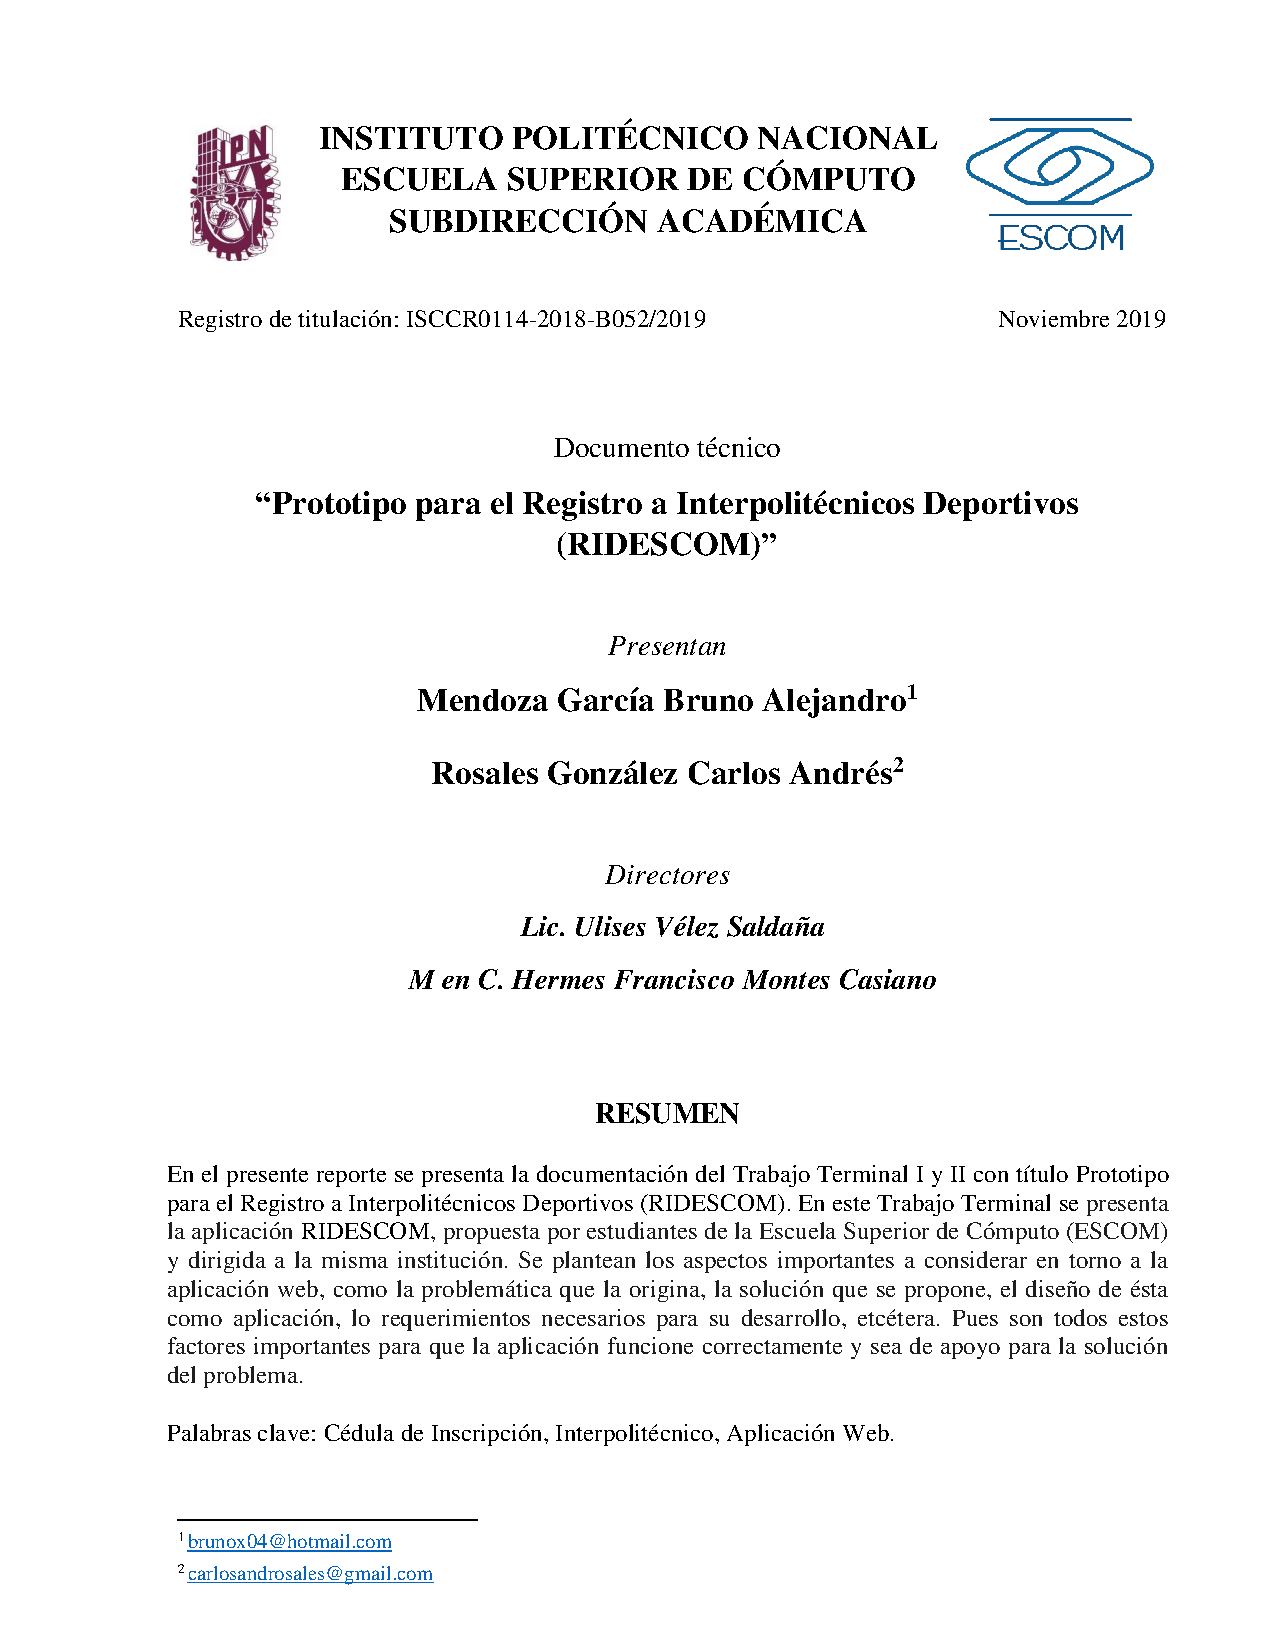
\includepdf{portada2.pdf}
	
	
\includepdf{cartaResponsivaTT20182.pdf}
	
	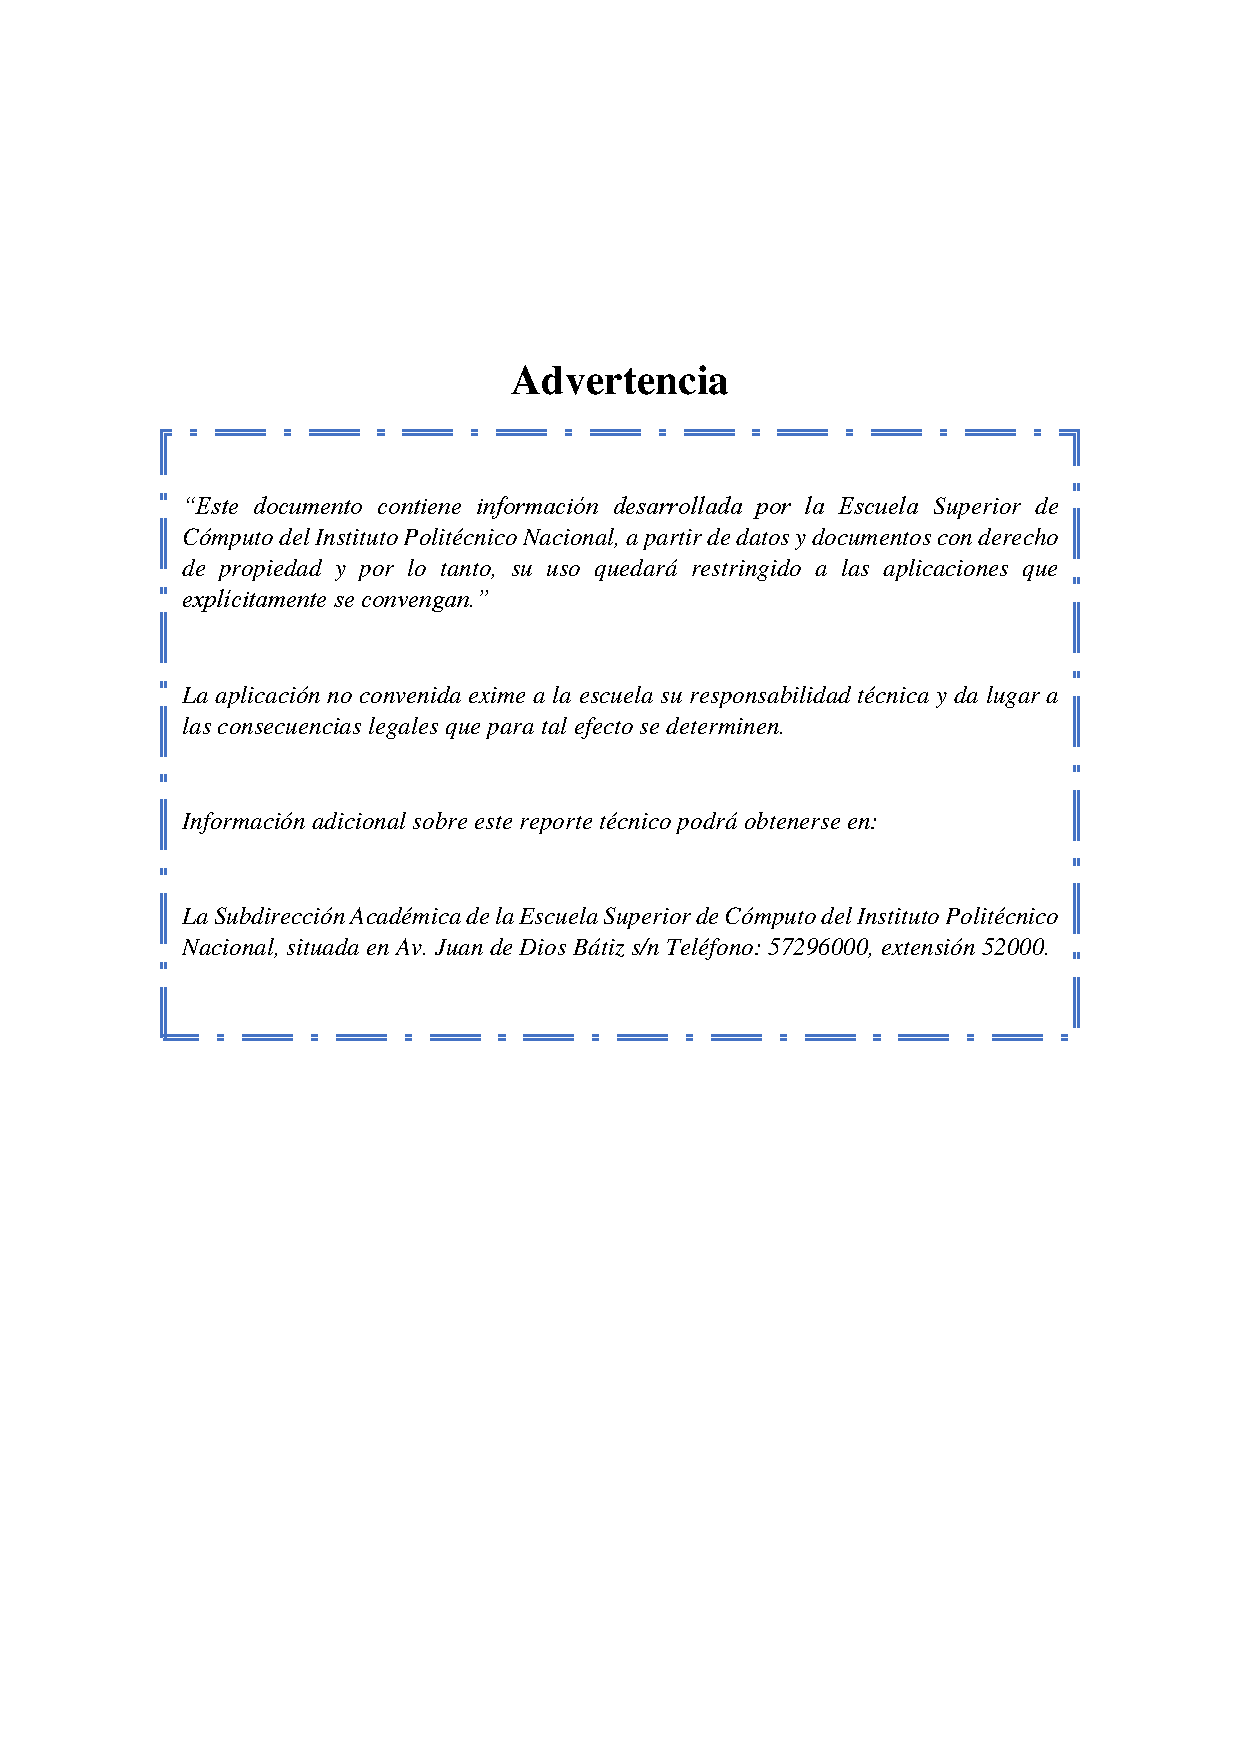
\includepdf{Advertencia.pdf}
	
	%=========================================================
	%                                                         Indice.
	%=========================================================
	
	\tableofcontents
	\mainmatter
		\chapter{Introducción}
	%=========================================================
	%                                                         Introduccion
	%=========================================================
	\section{Introducci\'on}
	
	\noindent Este documento presenta la aplicación web RIDESCOM, propuesta por estudiantes de la Escuela Superior de Cómputo (ESCOM) y dirigida para la misma institución. A lo largo del mismo se plantean aspectos importantes a considerar en torno a la aplicación, como puede ser la problemática que lo origina, las actividades que lo origina, las soluciones que se proponen, el diseño, la investigación realizada acerca de otras aplicaciones similares, los requerimientos necesarios para su desarrollo, etcétera. Pues son todos estos factores importantes para que la aplicación funcione correctamente y sea de apoyo a la solución del problema que más adelante se describirán detalladamente. Es en este apartado donde se explican las razones de ser el proyecto RIDESCOM, se describe el análisis que se lleva a cabo para posteriormente encontrar acciones y requerimientos, así como tecnologías necesarias para la creación de la aplicación. 
	Siendo así, se cuenta primeramente con un apartado de justificación, en el cual se exponen las razones y los diferentes problemas por los cuales RIDESCOM surge como medida para solucionar dichos problemas.\\
	Se detalla aquí la razón de nuestro proyecto, los diferentes caminos que podemos seguir para conseguir resultados favorables ante las problemáticas y los resultados que se espera tener cuando la aplicación llegue al usuario final. Es bien sabido que debemos enfocarnos en ellos, y en cómo tratar con los problemas para así encontrar la mejor solución, con los mejores beneficios y mayores resultados.\\
	Se establece un marco teórico en donde se describe el entorno en el cual se desarrolla el proyecto, el público al que va dirigida y las aplicaciones.\\
	Además se plantean las ideas y los problemas mismos que orillan a la creación de RIDESCOM para intentar solventarlos. Por otro lado se tiene también un análisis sobre las diferentes tecnologías y plataformas computacionales que nos ayudarán a realizar el proyecto, destacando la importancia de éstos y las consistencias en la aplicación y en los objetivos de la última. Por último, en este apartado se enlistan las diferentes palabras y términos que a lo largo del documento y en la propia aplicación se utilizan, así como una descripción de los mismos, con el objetivo de contextualizar al lector y comprender mejor la aplicación, su estructura, lo que ésta realiza y la interacción con el usuario final.\\
	En esta sección se muestra principalmente el trasfondo de la aplicación y las herramientas que se utilizan para su desarrollo. Se presentan las aplicaciones ya existentes que realizan tarea similares al proyecto RIDESCOM, el funcionamiento de las mismas, el público al que se dirigen y los propósitos que éstas consideran. Se realizan comparativas para encontrar aquellos puntos diferenciales en una aplicación y otra, y así implementar de la mejor manera en la aplicación las características con mayor importancia y que nos ayudarán a lograr los objetivos que más adelante se describirán.\\
	Se cuenta también con un capítulo dedicado a la aplicación propiamente dicha, en donde se describe la propuesta concreta de la aplicación, las acciones que ésta puede realizar, los usuarios que realizan una interacción con ella, así como las características y herramientas que en ella se contemplan para su funcionamiento. Se enlistan los objetivos general y específicos que se pretenden alcanzar con la aplicación, además es en este capítulo se tiene un primer gran acercamiento con el sistema, pues es aquí donde se analizan las acciones que se requieren y se empieza a descubrir y organizar los diferentes requerimientos funcionales y no funcionales que harán que RIDESCOM funcione apropiadamente, logre cumplir sus objetivos y así intentar solventar los problemas que propiciaron su existencia.\\
	Finalmente se cuenta con un apartado dedicado al análisis, diseño y desarrollo de la aplicación. En él se muestra el trabajo que se ha realizado desde que nació la idea hasta el presente día. Se detallan las diversas tareas realizadas para la comprensión del problema, las posibles soluciones, las aplicaciones similares, los prototipos de práctica previos al desarrollo de la aplicación. Aquí se concentran en forma de iteraciones toda acción que se realizó con fin de entender el propósito del proyecto, los diferentes conceptos referentes al análisis, diseño y desarrollo de RIDESCOM. Se muestran así, los avances que se tiene hasta hoy de la aplicación, los resultados a los que se ha llegado a lo largo de estos meses de trabajo, los cambios y los problemas que en él se han tenido, así como los logros que se han encontrado. Por último, se dedica una sección en este apartado para anunciar todo aquello que falta realizar y que se implementará en un futuro para que RIDESCOM se realice completa y exitosamente, y con ella los objetivos planteados, y a su vez solucionar aquellos problemas que en su momento fueron quien dieron pauta a la creación de la aplicación.\\
	Así como se explicó, en este documento nos encontramos con un proyecto que pretende servir y apoyar en ciertos aspectos de la Escuela Superior de Cómputo, así como la forma en que se estructura y las maneras en que se fue desarrollando.
	
	%=========================================================
	%                                                         Justificacion
	%=========================================================
	\section{Justificaci\'on}
	\noindent En este apartado se describen las razones y los  problemas por los cuales la aplicación RIDESCOM surge. Se detalla el “por qué” del proyecto, los diferentes caminos que podemos seguir para conseguir resultados favorables ante las problemáticas y los resultado que se espera tener cuando la aplicación llegue al usuario final. Así bien, a continuación se presenta la problemática que da origen a la aplicación.\\
	La aplicación web RIDESCOM está dirigida principalmente a los alumnos de la ESCOM que practiquen algún deporte impartido por la misma, aunque son los administrativos o responsables del área de departamento de fomento deportivo parte importante de la misma. Es importante establecer que, a pesar que la aplicación podrá ser utilizada por la comunidad en general,  el entorno en el que el usuario final se desarrolla es de suma importancia para la correcta comprensión del problema y de la solución propuesta con RIDESCOM.\\ 
	Así bien, debemos conocer y familiarizarnos con el entorno de la aplicación y los usuarios a los que está destinada. \\
	El Instituto Politécnico Nacional (IPN) es la institución educativa rectora de la educación tecnológica pública en México en los niveles medio superior, superior y posgrado. Tiene como misión formar integralmente capital humano capaz de ejercer el liderazgo en los ámbitos de su competencia, con una visión global, para contribuir al desarrollo social y económico de México. El Instituto se visualiza como una institución de vanguardia incluyente, transparente y eficiente que contribuye al desarrollo global, a través de sus funciones sustantivas, con calidad ética y compromiso social. A lo largo de su historia, el Politécnico se ha caracterizado por ser una Institución que ha evolucionado de acuerdo a las necesidades y realidades del país, reflejando en su imagen sus orígenes y razón de ser, lo que permite su fácil identificación por las personas y llegando a ser coloquialmente como “el Politécnico” o “el Poli”. \cite{hist} \\
	Es el IPN el alma mater de diferentes instituciones y escuelas públicas en México, tal es el caso de la Escuela Superior de Cómputo, escuela donde se procura que la formación de los estudiantes se integral, pues no solo imparten materias referentes a la formación orientada a sus carrera impartida (ingeniería en Sistemas Computacionales), sino contempla diferentes materias enfocadas a desarrollar diferentes aspectos y habilidades que los alumnos pueden poseer, proponiendo además, la posibilidad de participar en clubes y actividades deportivas y culturales. Es claro que la ESCOM se preocupa por lograr en sus alumnos una educación integral y de calidad. Sin embargo, ésto se ve opacado en numerosas ocasiones, pues a causa de la desorganización o mala comunicación entre los integrantes de la comunidad de la ESCOM, no se cumplen completamente el tener esta educación integral de la que se habla, siendo esto un problema. Pues en la ESCOM, además, la población tiende a ser individualista y aislada, provocando así barreras de comunicación y progreso. Dentro del plantel, las diferentes maneras de difusión de información pueden no ser las más óptimas, pues no se alcanza a distribuir de manera correcta a todos los integrantes de la comunidad, por poner un ejemplo, para la participación o inscripción a actividades deportivas, así como el participar en interpolitécnicos de la misma referente a la inscripción y el proceso que todo este conlleva y de esta manera aplicar soluciones para que no se presente más.\\
	Es por ello que se ha idealizado una solución que permita, entre otras cosas, compartir y conocer, así como agilizar los procesos de inscripción de inerpoliécnicos en la ESCOM.\\
	Así, queda claro que la aplicación RIDESCOM pretende informar y agilizar el proceso para inscribir un interpolitécnico, además de estar dirigida a quienes en primer plano sufren del problema anteriormente descrito, y son estos los propios alumnos del plantel.
	
	
	%=========================================================
	%                                                         Problematica
	%=========================================================
	\section{Problem\'atica}
	\noindent La educación es uno de los factores más importantes para el avance y progreso de las personas y sociedades. Además de proveer conocimientos, la educación enriquece la cultura y los valores. La educación es necesaria en todos los sentidos.\\
	La actividad deportiva dentro de las escuelas juega un factor importante dentro de la misma, sin embargo, en latinoamérica se presenta un alto índice de obesidad en los niños y jóvenes.  \cite{problemas}  Ahora bien, en México y específicamente la educación superior, se tiene participación de la comunidad estudiantil pero no es la gran parte con la que se cuenta. 
	(Poner referencia de escuelas o caso de estudio que se hayan realizado para justificar lo anterior y extender más la introduccion de la problemática.)\\
	Nuestro caso de estudio se enfoca en la ESCOM, para ello se realizó una entrevista con el Coordinador de Fomento Deportivo de ESCOM y con el Jefe del Departamento de Fomento Deportivo, con la finalidad de que se nos proporcionará datos de particpación por parte de los estudiantes, a la vez mencionar por los cuales se cree que no exita mayor participación en estos. Uno de los problemas que se tiene es el proceso actual para la inscripción de un interpolitécnico, este suele un poco tardado y fastidioso en cierto punto para el alumno, ya que este tiene que trámitar una constancia de estudios para que la pueda presentar al momento de ir a solicitar su inscripción a un evento interpolitécnico con el coordinador de la Unidad Académica.\\
	Otro de los problemas que tinene actualmente es el proceso de verificación del alumno (su estatus de inscripción), este punto es un requisito para poder participar,si el alumno no esta inscrito en el periodo actual no podrá participar en algun evento interpolitécnico. Sin embargo se mencionó que se llega a presentar el caso de que un alumno participe aun sin cumplir lo antes mencionado.
	Por último se mencionó que no hay un control en las personas que se registran para participar, ya que se a detectado la participación de personas ajenas a la institución. 
	
	%=========================================================
	%                                                         Problematica
	%=========================================================
	\section{Objetivos}
	\subsection{Objetivo General}
	\noindent Desarrollar una aplicación web de apoyo para el Departamento Deportivo de la Escuela Superior de Cómputo (ESCOM) que permita la inscripción de interpolitécnicos, visualizar los eventos próximos y a su vez sea un espacio de información y difusión.
	\subsection{Objetivos Especificos}
	\begin{itemize}
		\item Implementar un mecanismo de validación del estatus académico del alumno. 
		\item Implementar un módulo para la generación de la cédula de inscripción con base en el formato oficial de interpolitécnicos deportivos. 
		\item Implementar un módulo de comunicación con la red social (Facebook). 
		\item Implementar un módulo de consulta de resultados de competencias.
	\end{itemize}
		
	%=========================================================
	%                                                         Capitulo 2
	%=========================================================
		\chapter{Planteamiento del Problema}
\noindent En este capítulo se hablará de que es el Instituto Politécnico Nacional, como esta conformada, las actividades deportivas que en está se practican, así como los problemas que se tienen en estos úlitmos.
Con esto se presentará softwares que existen en el mercado que pueden ayudar a mitigar parte de los problemas existentes, sin embargo, como se mostrará no cubren en su totalidad los problemas existentas siendo así se presenta la solución propuesta por alumnos de la Escuela Superior de Cómputo.

%=========================================================
%                                                         Justificacion
%=========================================================
\section{Antecedentes}
\noindent El Instituto Politécnico Nacional (IPN) es una institución educativa del Estado creada para consolidar, a través de la educación, la Independencia Económica, Científica, Tecnológica, Cultural y Política para alcanzar el progreso social de la Nación, de acuerdo con los objetivos Históricos de la Revolución Mexicana, contenidos en la Constitución Política de los Estados Unidos Mexicanos.
\noindent En 1932 surgió la idea de integrar y estructurar un sistema de enseñanza técnica, proyecto en el cual participaron destacadamente el licenciado Narciso Bassols y los ingenieros Luis Enrique Erro y Carlos Vallejo Márquez.
\noindent Sus fundadores concibieron al Politécnico como un motor de desarrollo y espacio para la igualdad; apoyando por una parte, el proceso de industrialización del país y, por la otra, brindando alternativas educativas a todos los sectores sociales, en especial a los menos favorecidos​\cite{ipnMision}.
\noindent Actualmente el IPN está conformado por 46 Unidades Académica, considerando solo el Nivel Medio Superior y Nivel Superior. En cada una de ellas, además de seguir el plan de estudios correspondientes, se llevan a cabo distintas actividades deportivas con la finalidad de fomentar en los alumnos una mejor calidad de vida, así como el alejar a estos del consumo de drogas entre otros. \\
\noindent Se han creado eventos que fomentan la participación y competitividad de la comunidad, llamados interpolitécnicos. Estos involucran áreas tales como: actividades deportivas, culturales o académicas, dichos eventos son de participación gratuita y se realizan 2 veces al año entre todos los planteles académicos que constituyen al IPN, divididas en los niveles Medio Superior y Superior.  \cite{Reglas}\\
\noindent El IPN cuenta con 26 actividades deportivas registradas, sin embargo, en las unidades académicas no se practican todas y cada una de ellas.\cite{Reglas}.
\noindent Ahora bien, los Encuentros interpolitécnicos Deportivos son eventos en los que los alumnos participan como representantes de la unidad académica en la que estos formen su carrera profesional.\\
\noindent Estos se realizan cada ciclo escolar y se crea un evento para cada deporte, dependiendo de la cantidad de pruebas que tenga este se dividen en distintos días la realización de cada uno de ellos y a su vez tomando en cuenta la demanda.\\
\noindent La entidad dedicada a la coordinación de las actividades deportivas con las que cuenta el IPN, es la Dirección de Desarrollo y Fomento Deportivo \cite{DDyFD}. Esta se encarga de la creación, administración y control de todas las actividades deportivas prácticadas dentro del IPN tales como: definir el área donde se practican y la asignación de presupuesto de cada actividad deportiva, llevar un registro de la cantidad de población que practica un deporte. \cite{Reglamento}.	
\noindent A su vez coordinan la realización de los eventos Interpolitécnicos Deportivos del IPN siguiendo el reglamento general liga interpolitécnica. \cite{Reglamento}, donde se explican los  procesos que realiza cada persona involucrada.\\
\noindent El Coordinador de Área Deportiva de cada Unidad Académica es el responsable de supervisar los aspectos operativos y técnicos de todos los deportes que se practican dentro de la misma así mismo es el encargado de realizar el proceso de inscripción a un interpolitécnico para los alumnos que así lo deseen y para que puedan participar este deberá solicitar la documentación de inscripción (cédula de inscripción) individual o de sus equipos y entregarlos a los Coordinadores de cada Disciplina Deportiva en la Dirección de Desarrollo y Fomento Deportivo. \cite{Reglamento} \\
\noindent  El alumno que desee participar en un evento interpolitécno deberá acudir con el coordinador de su unidad académica para comenzar el proceso de inscripción a un evento interpolitécnico. 
\\El coordinador le solicitará una forma para comprobar su estatus académico, este puede variar dependiendo de los coordinadores de las distintas unidades académicas. A su vez el alumno llenará el formato de inscripción al evento de su interés, anexando una fotografía. 
\\ Si se comprueba que el alumno está inscrito en el periodo actual en el que quiere participar, podrá continuar con el proceso, en caso contrario se negará la inscripción. \cite{Reglamento}
\\ Al concluir con la comprobación de inscripción, se le notifica al alumno cual es el estatus de su solicitud. 

\noindent Para más detalles puede consultarse en el apartado Anexos Apartado \ref{ProcesoInscripcionActual}


%=========================================================
%                                                         Problematica
%=========================================================
\section{Problem\'atica}
\noindent La educación es uno de los factores más importantes para el avance y progreso de las personas y sociedades. Además de proveer conocimientos, la educación enriquece la cultura y los valores. La educación es necesaria en todos los sentidos.\\
La actividad deportiva dentro de las escuelas juega un factor importante dentro de la misma, sin embargo, en latinoamérica se presenta un alto índice de obesidad en los niños y jóvenes.  \cite{problemas}  Ahora bien, en México y específicamente la educación superior, se tiene participación de la comunidad estudiantil pero no es la gran parte con la que se cuenta.\\
Nuestro caso de estudio se enfoca en la ESCOM, para ello se realizó una entrevista con el Coordinador de Fomento Deportivo de ESCOM y con el Jefe del Departamento de Fomento Deportivo, con la finalidad de que se nos proporcionará datos de particpación por parte de los estudiantes, a la vez mencionar por los cuales se cree que no exita mayor participación en estos. Uno de los problemas que se tiene es el proceso actual para la inscripción de un interpolitécnico, este suele un poco tardado y fastidioso en cierto punto para el alumno, ya que este tiene que trámitar una constancia de estudios para que la pueda presentar al momento de ir a solicitar su inscripción a un evento interpolitécnico con el coordinador de la Unidad Académica.\\
Otro de los problemas que tinene actualmente es el proceso de verificación del alumno (su estatus de inscripción), este punto es un requisito para poder participar,si el alumno no esta inscrito en el periodo actual no podrá participar en algun evento interpolitécnico. Sin embargo se mencionó que se llega a presentar el caso de que un alumno participe aun sin cumplir lo antes mencionado.
Por último se mencionó que no hay un control en las personas que se registran para participar, ya que se a detectado la participación de personas ajenas a la institución. 


%=========================================================
%                                                         Justificacion
%=========================================================
\section{Justificaci\'on}

\noindent La aplicación web RIDESCOM está dirigida principalmente a los alumnos de la ESCOM que practiquen algún deporte impartido por la misma escuela, aunque los administrativos o responsables del área del departamento de fomento deportivo forman parte importante de la misma. Es importante establecer que, a pesar que la aplicación podrá ser utilizada por la comunidad en general,  el entorno en que el usuario final se desarrolla es de suma importancia para la correcta comprensión del problema presentado y de la solución propuesta con RIDESCOM.\\ 
Así bien, debemos conocer y familiarizarnos con el entorno de la aplicación y los usuarios destinados. \\
El Instituto Politécnico Nacional (IPN) es la institución educativa rectora de la educación tecnológica pública en México en los niveles medio superior, superior y posgrado. \cite{hist} \\

El IPN el alma mater de diferentes instituciones y escuelas públicas en México, tal es el caso de la Escuela Superior de Cómputo, escuela donde se procura que la formación de los estudiantes sea integral, pues no solo imparten materias referentes a la formación orientada a sus carrera impartida (ingeniería en Sistemas Computacionales), sino contempla diferentes materias enfocadas a desarrollar diferentes aspectos y habilidades que los alumnos pueden poseer, proponiendo además, la posibilidad de participar en clubes y actividades deportivas y culturales. \\ 
Es importante impulsar la participación de la comunidad en alguna de las áreas mencionadas 
Es por ello que se ha idealizado una solución que permita compartir y conocer, así como agilizar los procesos de inscripción de inerpoliécnicos en la ESCOM.\\ %%aclarar mejor
Así, queda claro que la aplicación RIDESCOM pretende informar y agilizar el proceso para inscribir un interpolitécnico, además de estar dirigida a quienes en primer plano sufren del problema anteriormente descrito, y son estos los propios alumnos del plantel.


%=========================================================
%                                                         Estado del arte
%=========================================================
%\section{Estado del arte}
\noindent En esta sección se describen las aplicaciones web existentes en el mercado que se apeguen con el tema del presente Trabajo Terminal, con la finalidad de saber si existe una aplicación que cubra con los problemas que atañe este trabajo terminal o en su defecto, ver que caracteristicas se pueden tomar como base para agregar o mejorar y así dar solución a los problemas que ataca el proyecto. 


%=========================================================
%                                                         Historia
%=========================================================
%\section{Historia}


%=========================================================
%                                                         Aplicaciones
%=========================================================
\section{Aplicaciones}
\noindent Dentro de la investigación que se realizó con respecto a sistemas o aplicaciones web que tuviesen el mismo objetivo al proyecto propuesto. A continuación se muestran las aplicaciones que se encontraron, así como una descripción de su funcionamiento y las principales caracteristicas de cada una de ellas.
\subsection{Aplicaciones Tournament Software}
\noindent Esta aplicación ofrece al usuario un plataforma en la que puede registrar equipos deportivos, a su vez le ofrece crear ligas (competencias) entre los equipos que previamente registro, agregando que al final le dará una tabla de posiciones de los equipos y si este desea ver más información de uno en particular, desglosar la información en otra vista. \cite{ts}
Características: 
\begin{itemize}
	\item Login: Necesario para que el coordinador de los equipos registren los equipos que dirigen.
	\item Registro de equipos: Necesario para poder generar eventos entre los equipos registrados.
	\item Creación de eventos: Se necesita tener equipos registrados para poder eventos entre los distintos equipos.
	\item Consulta de resultados: Una vez concluido los eventos, da la opción de registrar los resultados para su consulta.
\end{itemize}
\pagebreak
%=========================================================
%                                                         Imagenes
%=========================================================
\begin{figure}[h]
	\centering
	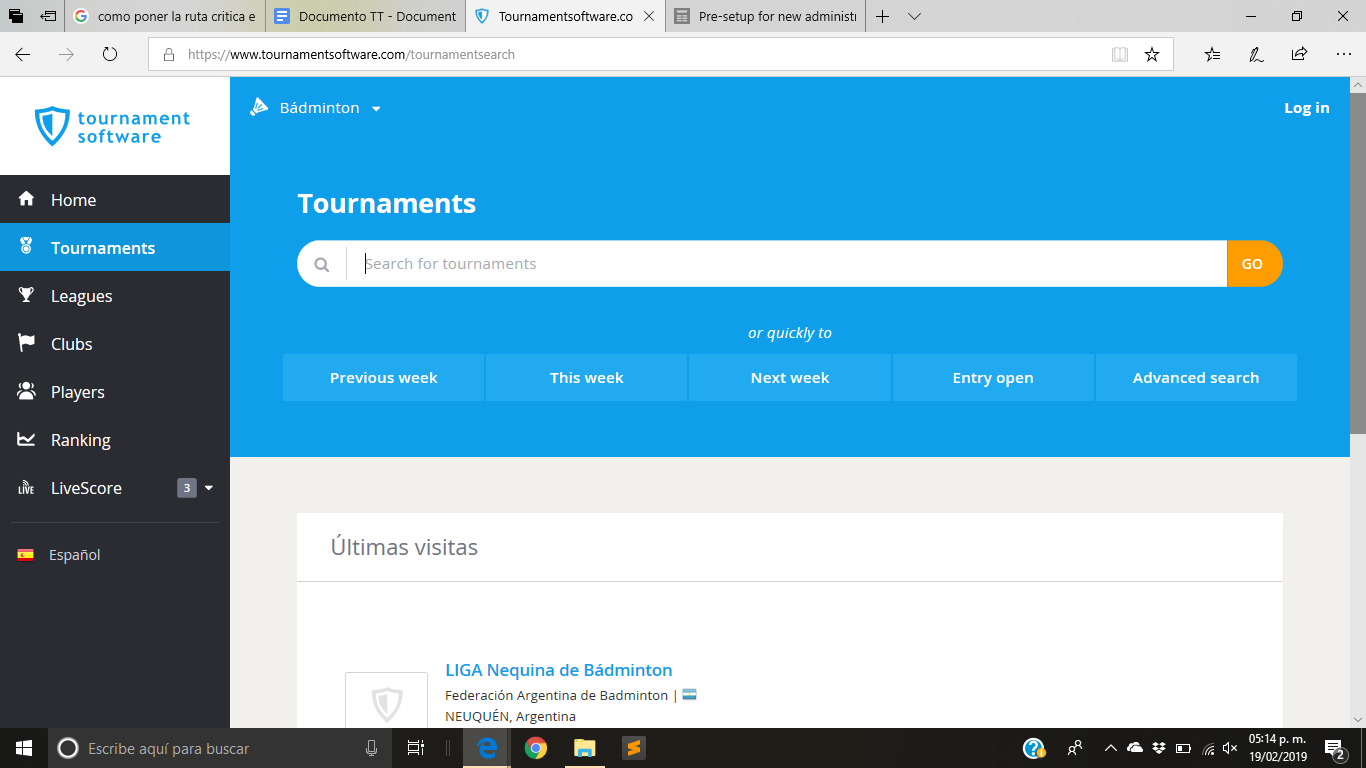
\includegraphics[width=12cm, height=6cm]{Imagenes/Aplicaciones/ToS1.png}
	\caption{Eventos registrados}
\end{figure}
\begin{figure}[h]
	\centering
	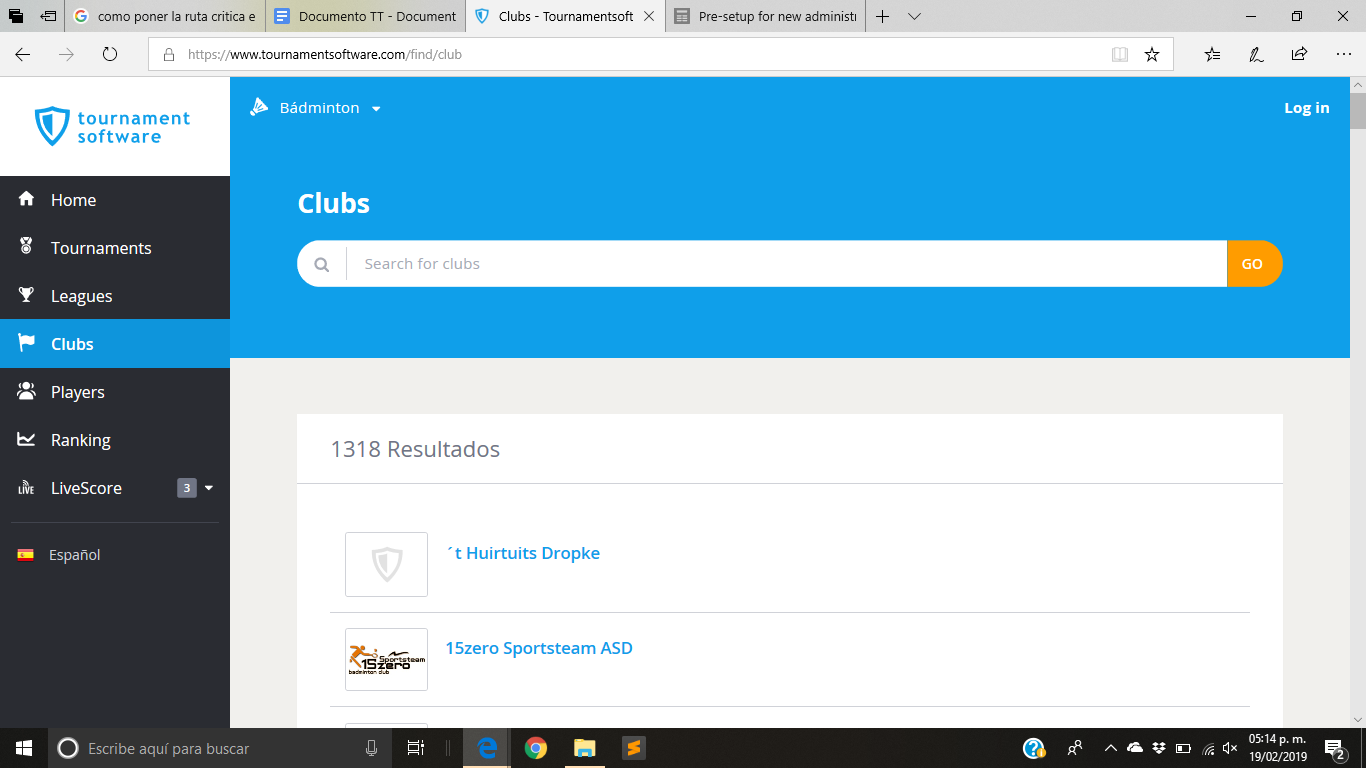
\includegraphics[width=12cm, height=6cm]{Imagenes/Aplicaciones/ToS2.png}
	\caption{Clubs registrados}
\end{figure}
\pagebreak
\begin{figure}[h]
	\centering
	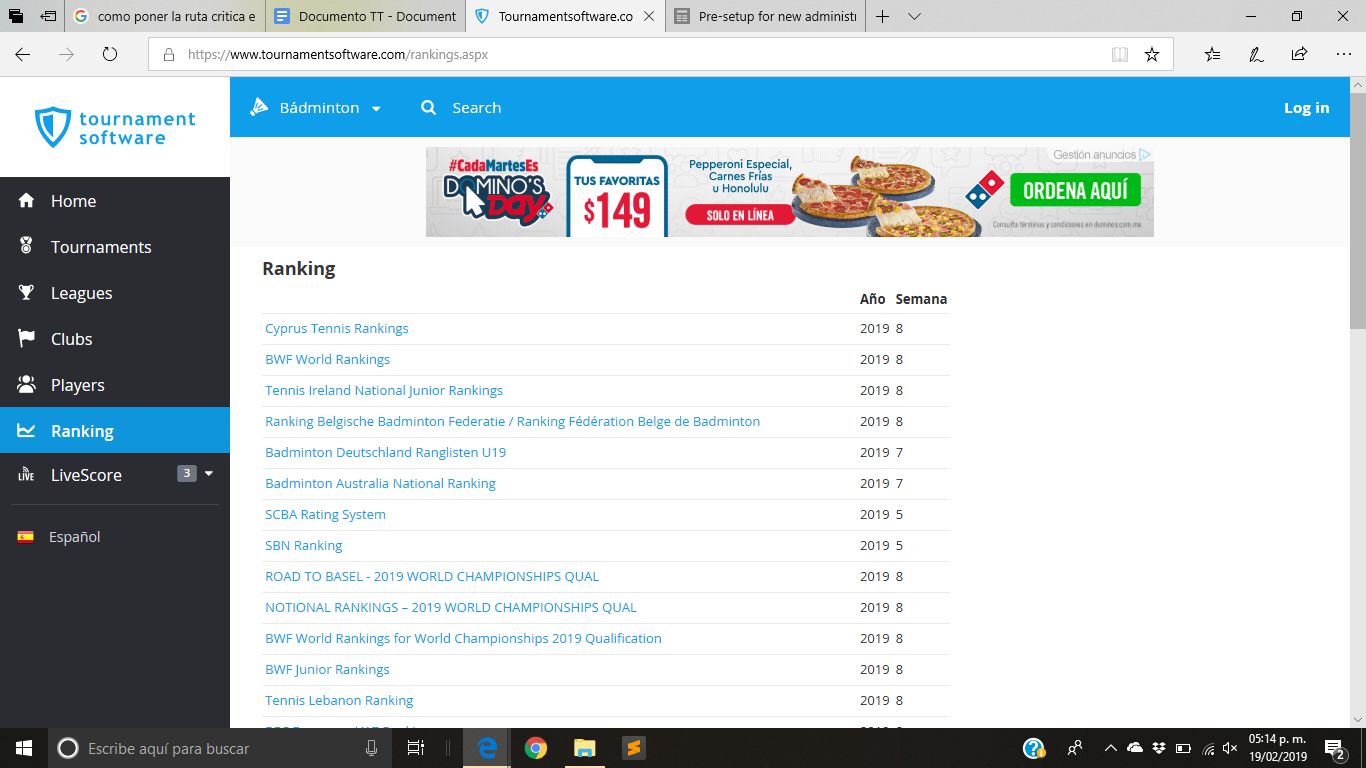
\includegraphics[width=12cm, height=6cm]{Imagenes/Aplicaciones/Tos3.png}
	\caption{Resultados}
\end{figure}

\subsection{Aplicaciones Active Network}
\noindent Esta aplicación ofrece a los usuarios de un manera organizada y fácil, el controlar alguna actividad deportiva, a su vez tienen un mercado más amplio ya que ofrecen sus servicio a escuelas, eventos deportivos, entre otros. Una desventaja que se encontró, es que para cada actividad deportiva se tiene una página designada, que es independiente al resto. \cite{act}
Características: 
\begin{itemize}
	\item Login: Necesario para poder registrar, crear eventos.
	\item Calendario: Muestra los eventos próximos previamente registrados.
	\item Registro de equipos: Permite dar de alta equipos.
	\item Reportes: Generar reportes al final de los eventos.
	\item Registro de eventos: Crea eventos que involucran a los equipos registraos.
\end{itemize}
%=========================================================
%                                                         Imagenes
%=========================================================
\begin{figure}[ht]
	\centering
	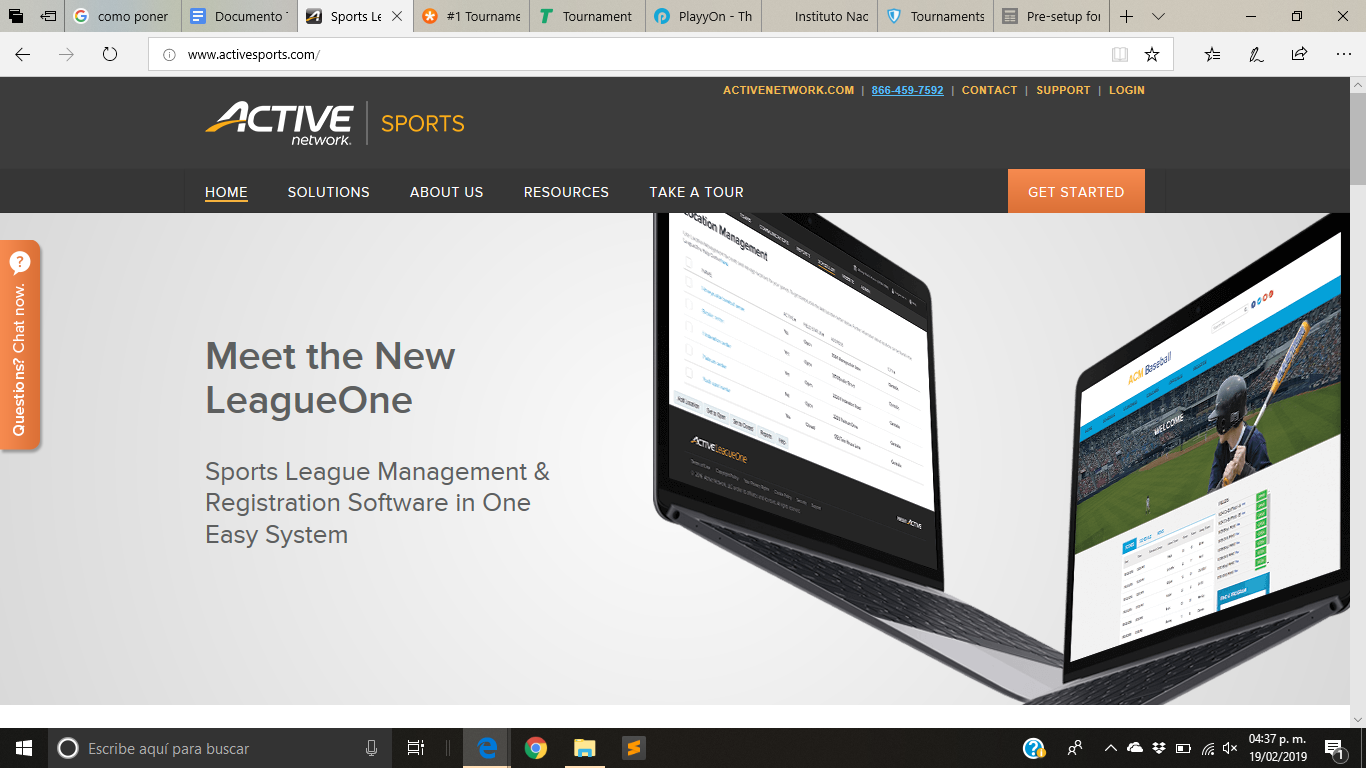
\includegraphics[width=12cm, height=6cm]{Imagenes/Aplicaciones/AN1.png}
	\caption{Página principal}
\end{figure}

\pagebreak

\begin{figure}[ht]
	\centering
	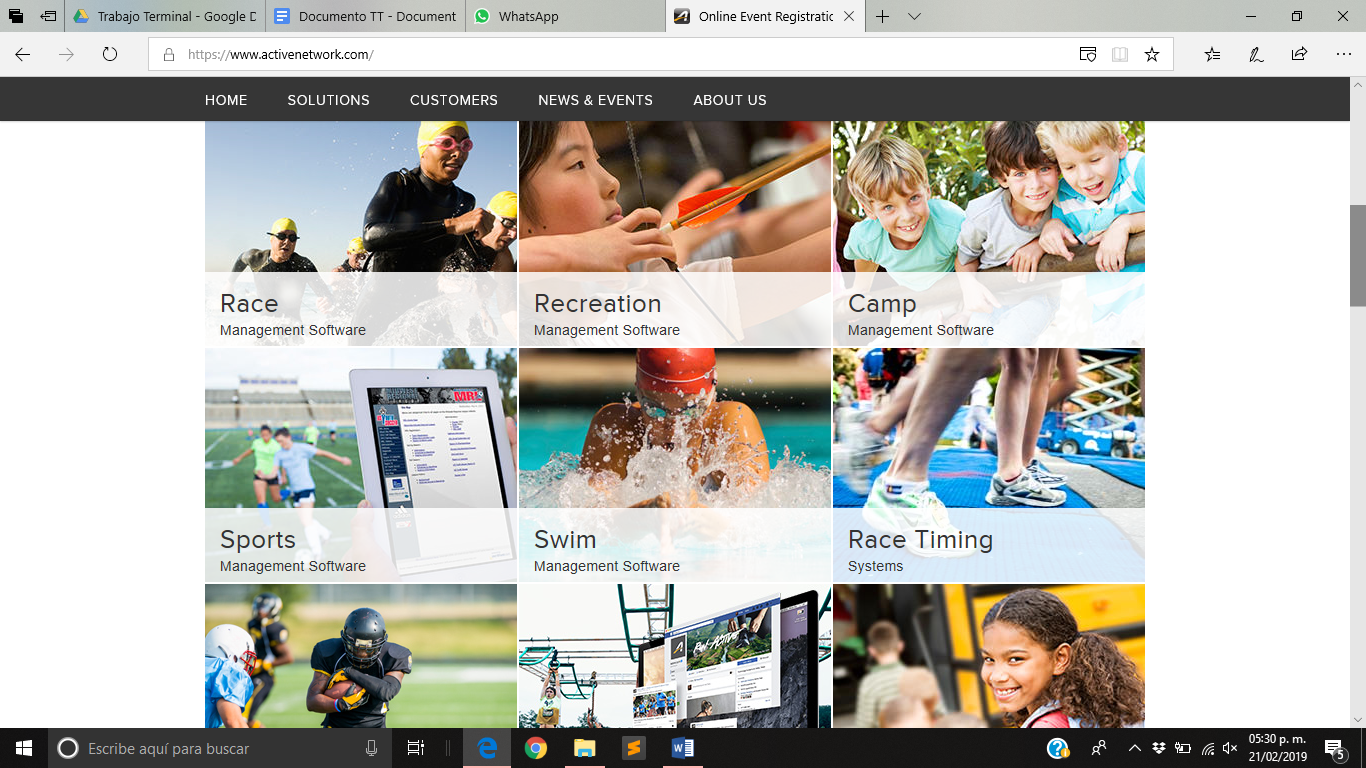
\includegraphics[width=12cm, height=6cm]{Imagenes/Aplicaciones/AN2.png}
	\caption{Eventos deportivos}
\end{figure}


\subsection{Aplicaciones TeamSnap Tournament}
\noindent La aplicación ofrece a los usuarios, un espacio en donde pueden registrar eventos deportivos, agendar o llevar control en el calendario de eventos, saber tablas de posiciones (estadísticas), otra característica de esta aplicación es que tiene un apartado en donde el administrador puede definir el precio de la inscripción a los eventos. \cite{team}
Características: 
\begin{itemize}
	\item Creación de eventos: Generar eventos para que posteriormente los interesados puedan inscribirse.
	\item Dar precio para inscripción a un evento: Permite asignar un monto monetario, si asi se desea para la inscripción a un evento.
	\item Cédula de inscripción: Permite generar el formato de inscripción para los distintos eventos.
	\item Difusión: Una vez creado un evento, se permite promocionar el evento dentro de la misma página.
\end{itemize}
%=========================================================
%                                                         Imagenes
%=========================================================
\begin{figure}[hbt]
	\centering
	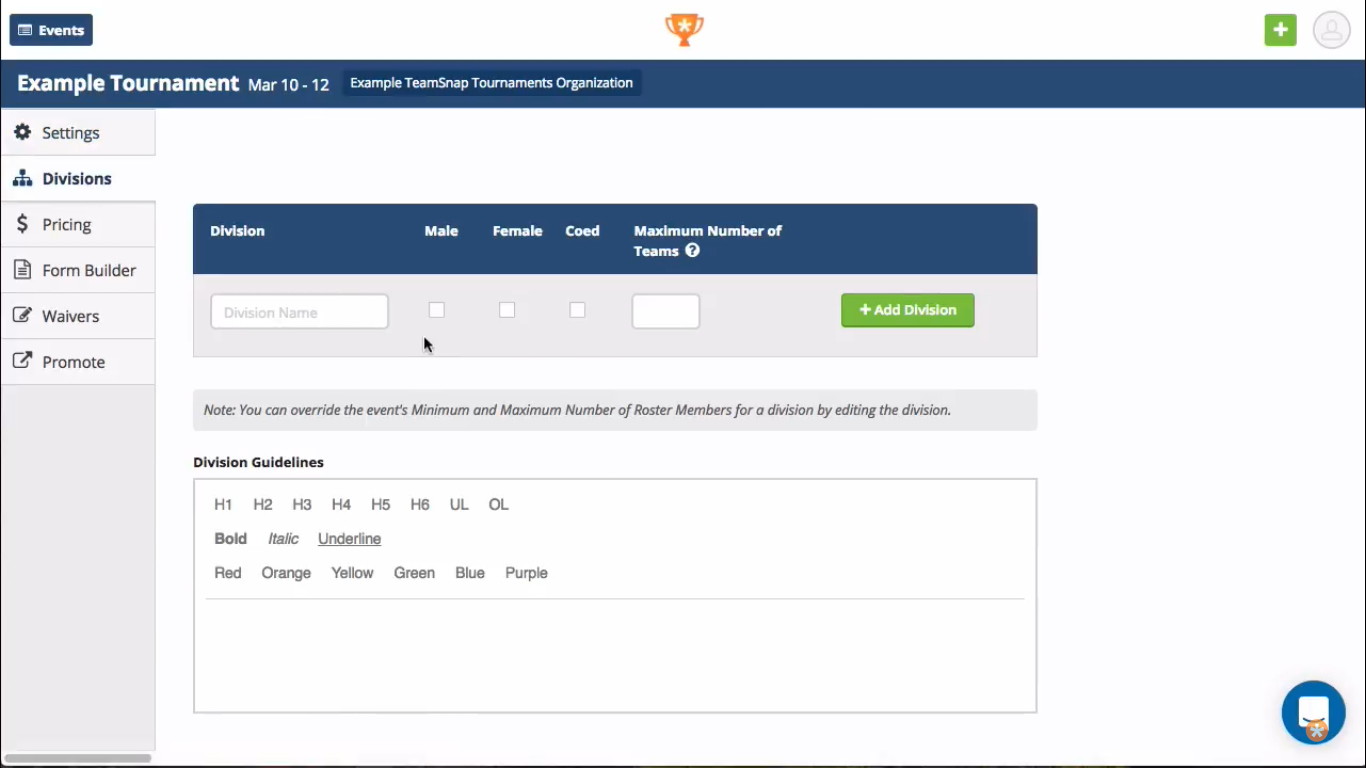
\includegraphics[width=12cm, height=6cm]{Imagenes/Aplicaciones/TsT1.png}
	\caption{Registro de competencias}
		\label{Imagen}
\end{figure}
\pagebreak
\begin{figure}[hbt]
	\centering
	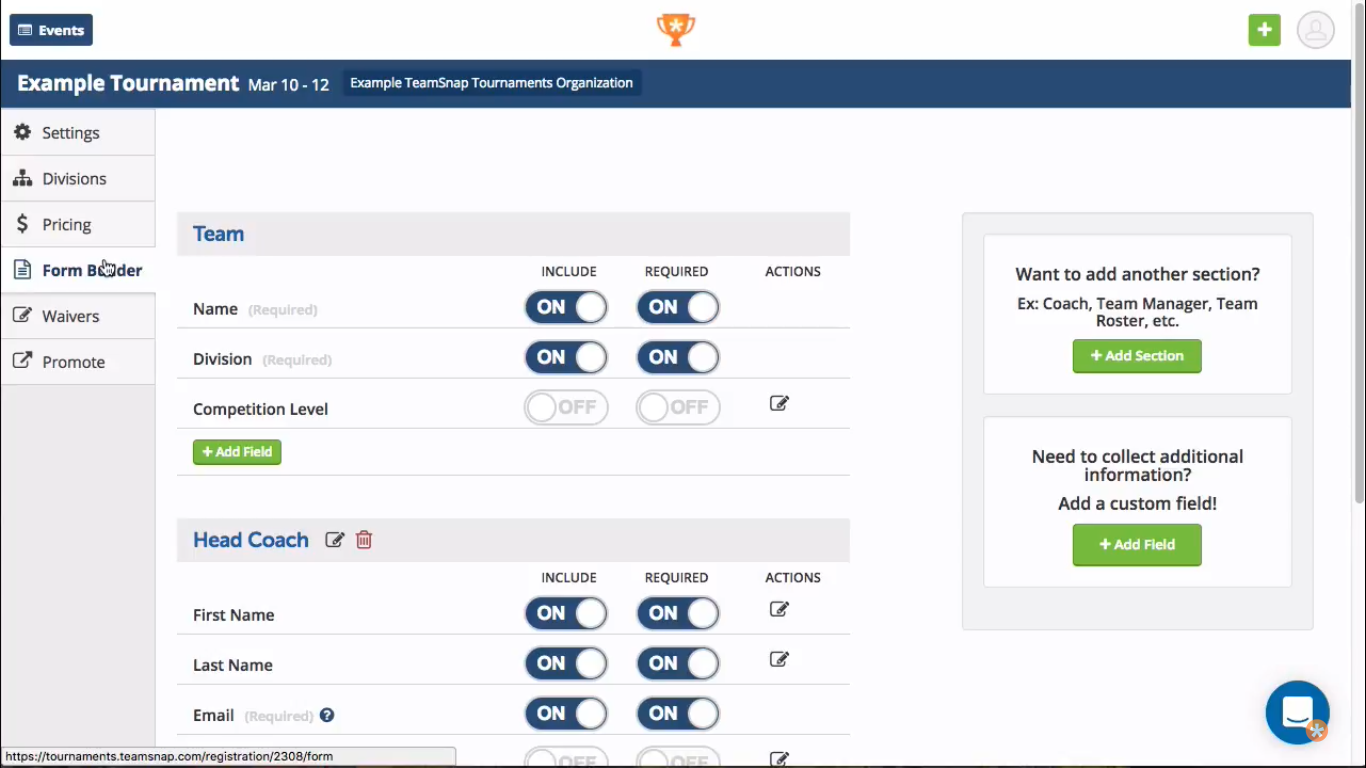
\includegraphics[width=12cm, height=6cm]{Imagenes/Aplicaciones/TsT2.png}
	\caption{Creación de cédula de inscripción}
\end{figure}
\begin{figure}[hbt]
	\centering
	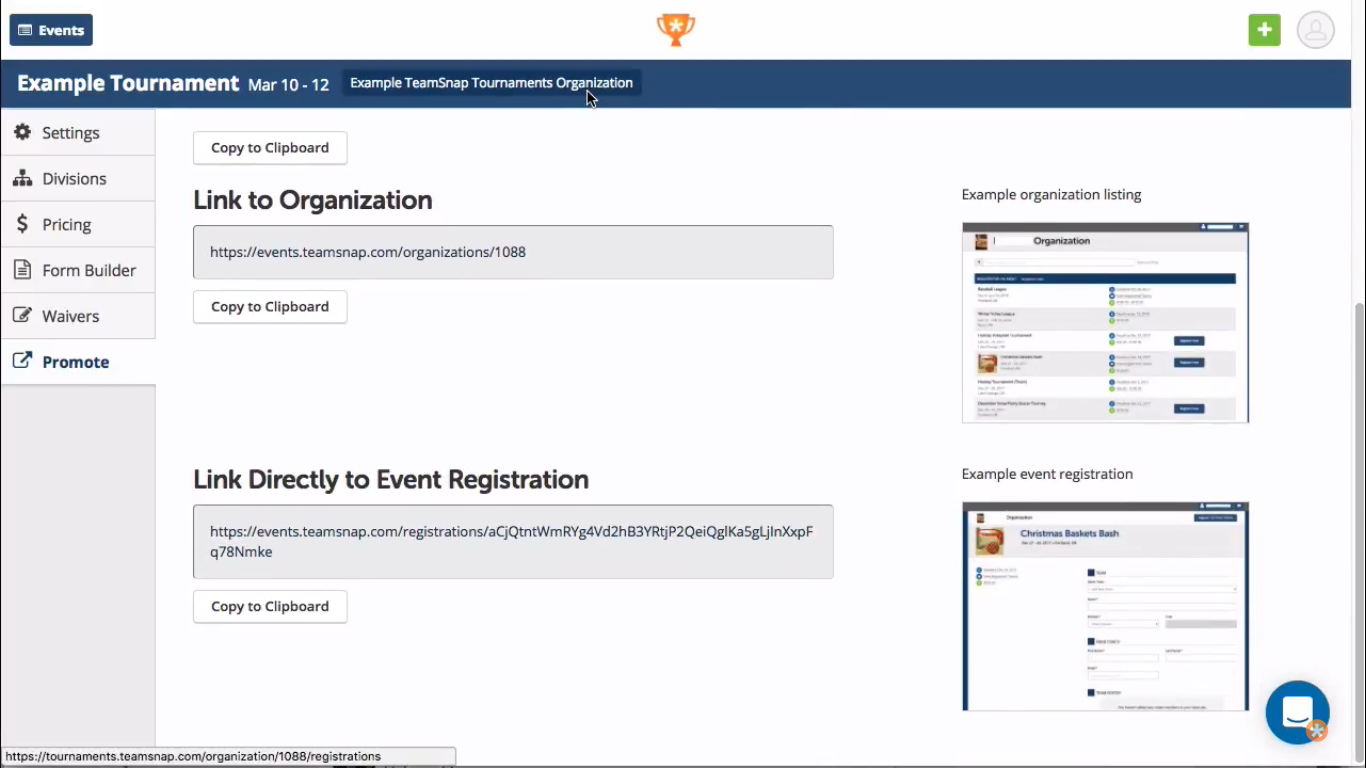
\includegraphics[width=12cm, height=6cm]{Imagenes/Aplicaciones/TsT3.png}
	\caption{Promover}
\end{figure}
\pagebreak


\subsection{Aplicaciones TorneoPal}
\noindent Esta aplicación, al igual que las anteriores, ofrece a los usuarios el generar un horario de actividades, generar torneos entre los equipos registrados y a su vez, en el apartado de estadísticas, ver en una tabla general el estatus de los equipos. \cite{tp}
Características: 
\begin{itemize}
	\item Creación de eventos: Permite crear eventos y asignar, si lo desea un límite de edad para los participantes, el número máximo de integrantes por equipo entre otras características.
	\item Resultados: Una vez concluido los eventos se puede ingresar los resultados para que puedan ser visualizados.
	\item Eliminar eventos: En caso de que se desee, se puede eliminar un evento.
	\item Cambio de equipo en categorías: Se puede modificar un evento, en este caso modificar la categoría en la que se participará.
	\item Informe a árbitros: Se le informa al personal de árbitraje de los eventos que han sido asignados.
	\item Calendario: Muestra los eventos próximos registrados.
	
\end{itemize}
%=========================================================
%                                                         Imagenes
%=========================================================
\begin{figure}[h!]
	\centering
	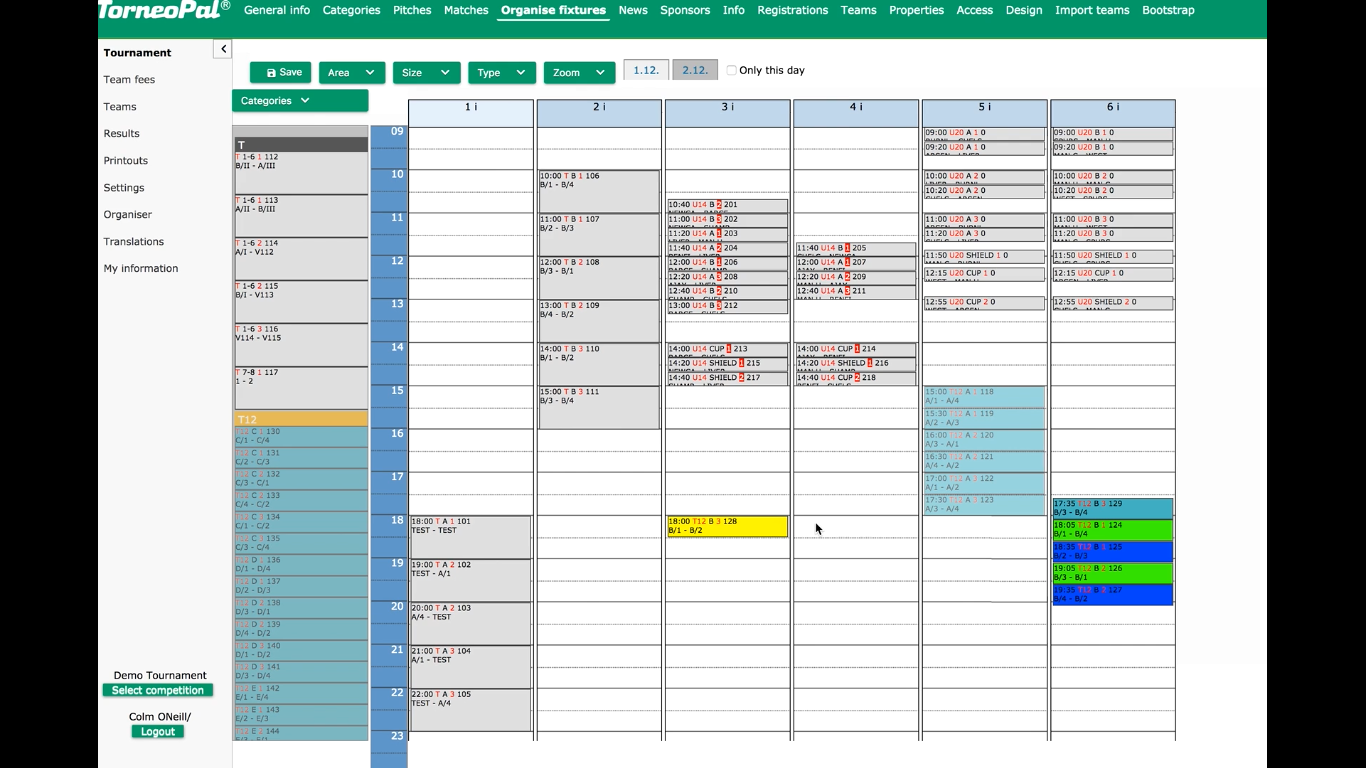
\includegraphics[width=12cm, height=6cm]{Imagenes/Aplicaciones/TP1.png}
	\caption{Calendario de eventos}
\end{figure}
\begin{figure}[h!]
	\centering
	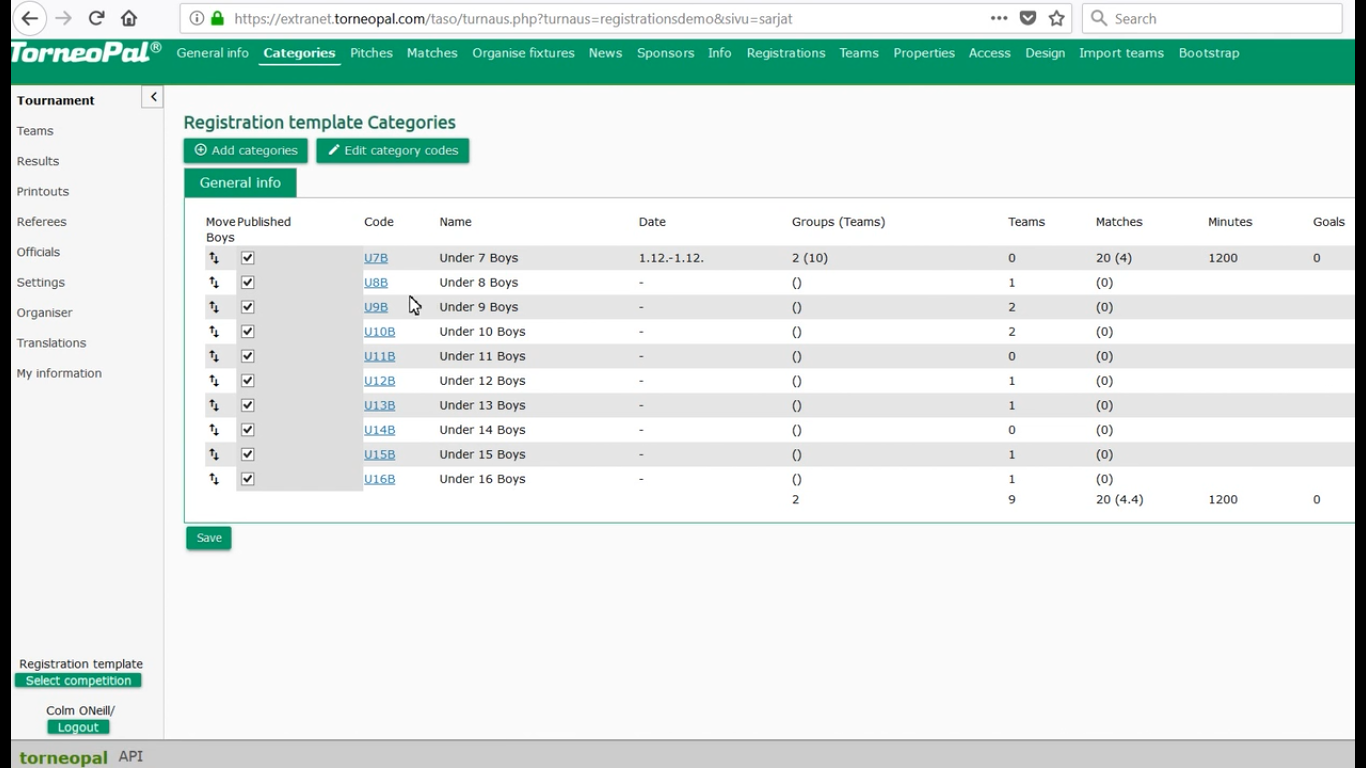
\includegraphics[width=12cm, height=6cm]{Imagenes/Aplicaciones/TP2.png}
	\caption{Registro eventos}
\end{figure}
\pagebreak

\subsection{Aplicaciones Instituto Nacional del deporte CHILE}
\noindent Esta aplicación está dirigida a un mercado en específico, ofreciendo dentro de esta un calendario de próximos eventos, registrarse en alguno del interés del usuario, como complemento se informa los requisitos para poder participar en los eventos y  un apartado en donde pueden dar de alta a organizaciones. No cuenta con un apartado donde muestre estadísticas. \cite{IND}
Características: 
\begin{itemize}
	\item Registro: Dirigido a los estudiantes que deseen participar en los eventos ya registrados.
	\item Calendario: Muestra de manera general los eventos próximos.
	\item Informes: Proporciona información general a los interesados.
	
\end{itemize}
%=========================================================
%                                                         Imagenes
%=========================================================
\begin{figure}[hbt!]
	\centering
	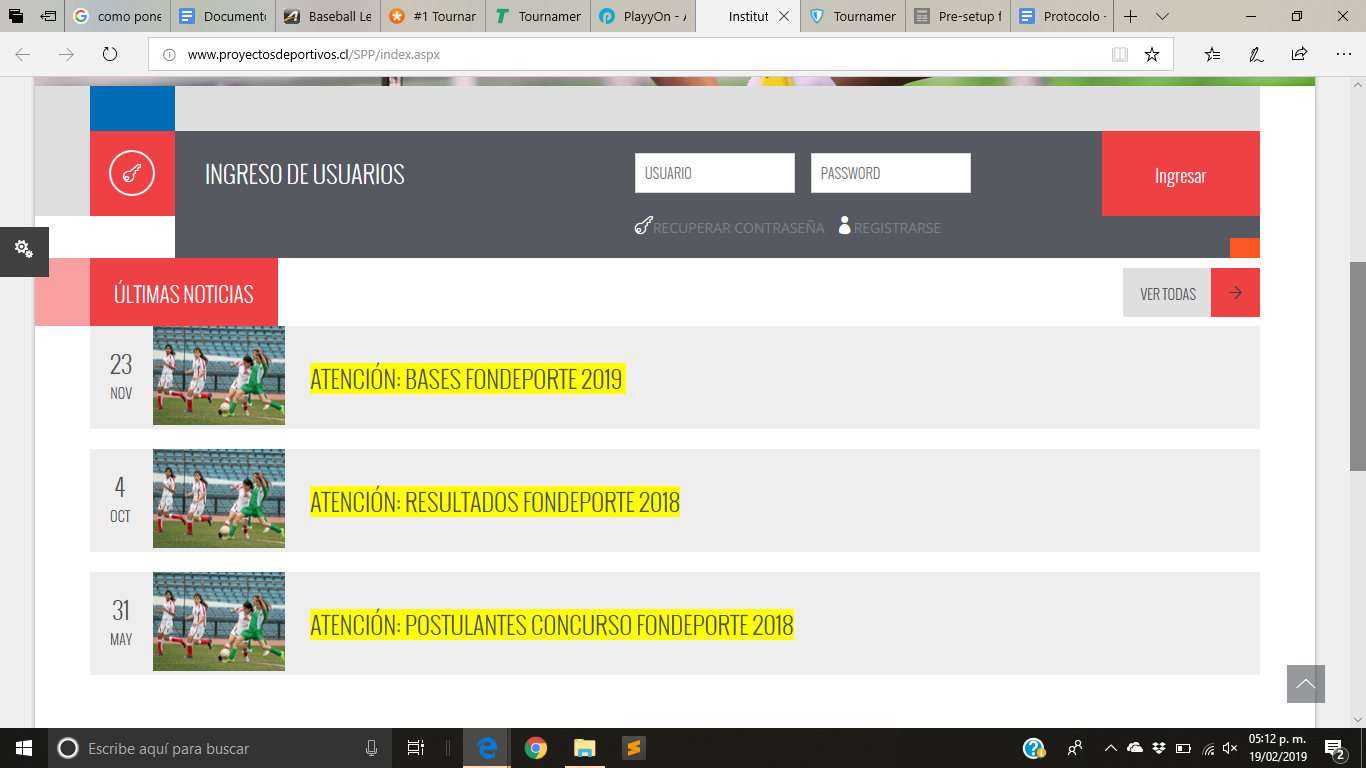
\includegraphics[width=12cm, height=6cm]{Imagenes/Aplicaciones/INDC1.png}
	\caption{Calendario de eventos}
\end{figure}
\begin{figure}[hbt!]
	\centering
	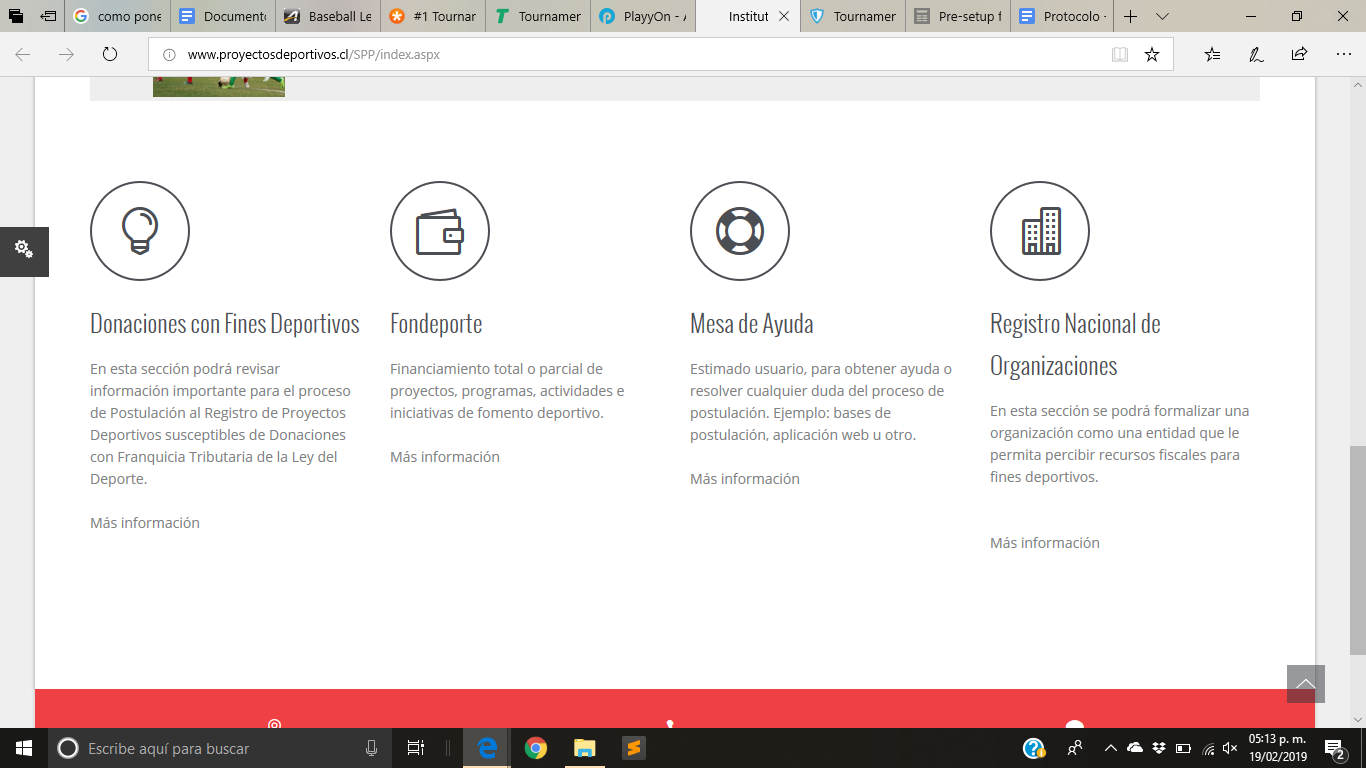
\includegraphics[width=12cm, height=6cm]{Imagenes/Aplicaciones/INDC2.png}
	\caption{Contacto}
\end{figure}
\pagebreak

\subsection{Prototipo para el registro a interpolitécnicos RIDESCOM}
\noindent Esta aplicación esta dirigida a la comunidad del Instituto Politécnico Nacional, especificamente en la Escuela Superior de Cómputo. La cual ofrece a la comunidad un espacio donde pueda ver el calendario de eventos próximos, resultados de la comunidad que participó, así como la posibilidad de inscribirse a un evento cuando estos esten disponibles. 
\\Dentro de la investigación se encontró características en común en todas las aplicaciones, que para nuestro caso en particular ayuda a atacar la problemática, sin embargo ninguna de ellas cumple con todos los requisitos que se busca, ya sea porque no cumple con todos los puntos o en algunos casos, es necesario realizar una subscripción para poder hacer uso del servicio que se ofrece. Sin embargo se puede tomar como punto de referencia algunos casos para ser implementados en nuestra aplicación.
Las características que pretende tener nuestro proyecto son las siguientes:
\begin{itemize}
	\item Registro de eventos: Crear eventos deportivos para que los interesados puedan inscribirse en estos.
	\item Calendario de eventos: Se mostrará los eventos que ya han sido registrados.
	\item Resultados: Una vez que se concluyan los eventos, podrán ingresar los resultados de los participantes para que pueda ser vistos por la comunidad escolar.
	\item Inscripción a eventos: Permitir a los alumnos interesados inscribirse en el evento de su interes. 
\end{itemize}

\noindent A continuación se muestra una tabla comparativa, en la que se muestran las caracteristicas de las aplicaciones antes mencionadas y el proyecto propuesto. Para más detalles consulte la \ref{tablacomparativa}.

\begin{figure} [hbt!]
	\centering
	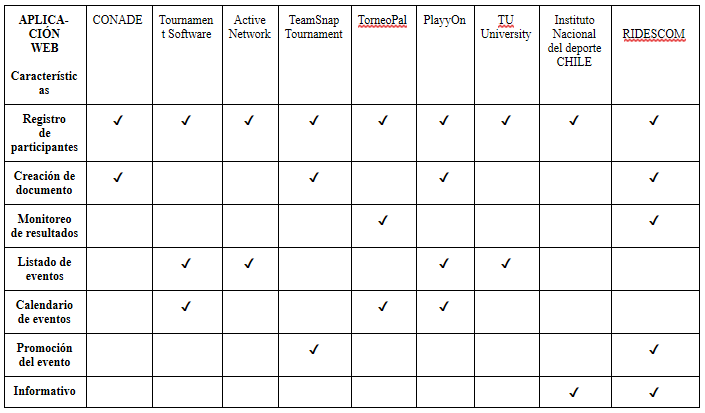
\includegraphics[width=15cm, height=6cm]{Imagenes/tablaComparativa}
	\caption{Caracteristicas principales de las páginas similares.}
	\label{tablacomparativa}
\end{figure}

\noindent El problema que resuelve el trabajo terminal es: la inscripción de personas ajenas al Instituto Politécnico Nacional, la comprobación del estatus académico de los participantes con base ene el reglamento que propuso el Departamento de Fomento Deportivo.
	%=========================================================
	%                                                         Capitulo 3 Estado del arte
	%=========================================================
		\chapter{Propuesta de solución}

%=========================================================
%                                                         Problematica
%=========================================================
\section{Objetivos}
\noindent En esta sección se menciona el objetivo general y los objetivos especifícos, los cuales ayudarán a atacar la problemática.
\subsection{Objetivo General}
\noindent Desarrollar una aplicación web de apoyo para el Departamento Deportivo de la Escuela Superior de Cómputo (ESCOM) que permita la inscripción de interpolitécnicos, visualizar los eventos próximos y a su vez sea un espacio de información y difusión.
\subsection{Objetivos Especificos}
\begin{itemize}
	\item Implementar un mecanismo de validación del estatus académico del alumno. 
	\item Implementar un módulo para la generación de la cédula de inscripción con base en el formato oficial de interpolitécnicos deportivos. 
	\item Implementar un módulo de comunicación con la red social (Facebook). 
	\item Implementar un módulo de consulta de resultados de competencias.
\end{itemize}
\pagebreak

	%=========================================================
	%                                                         Marco teorico
	%=========================================================
	\section{Alcance de la solución}
	\noindent En la Figura \ref{arquitectura} se muestra la arquitectura de la aplicación web,
	\begin{figure}[hbt!]
		\centering
		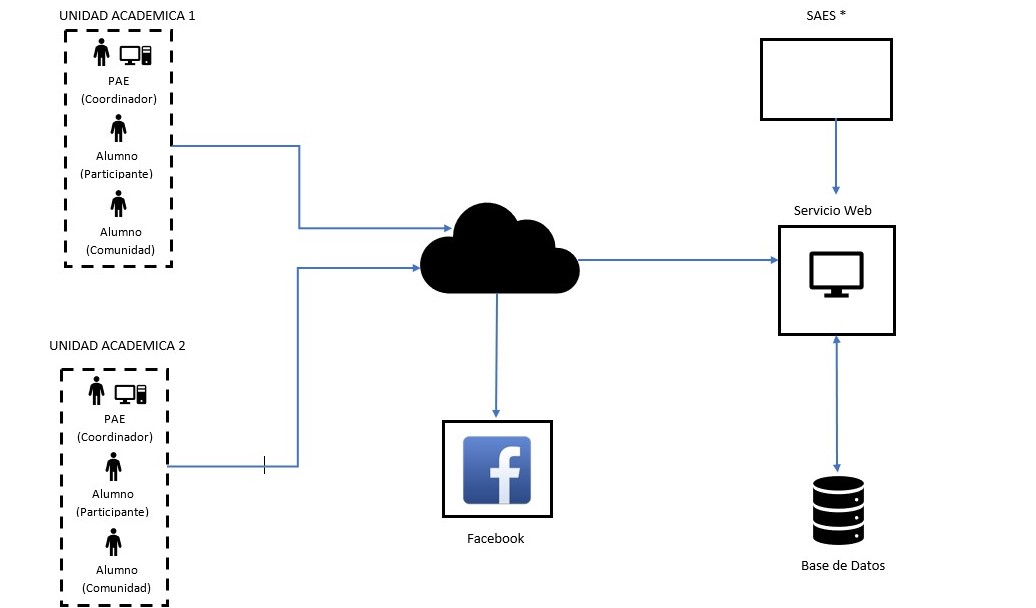
\includegraphics[width=10cm, height=6cm]{Imagenes/arquitectura}
		\caption{Arquitectura del sistema}
		\label{arquitectura}
	\end{figure}

	\noindent Como se puede observar, esta contempla su implementación en otras unidades académicas, sin embargo cabe mencionar que el Trabajo Terminal se enfocará particularmente en ESCOM con el objetivo de análisar, estudiar la aceptación del mismo, así como posibles mejoras.
	
	\noindet La aplicación esta involucrada por 3 usuarios, el Jefe de Departamento de Fomento Deportivo, el coordinador de Unidad Académica y el alumno. En esta cada uno tendrá distintos permisos y funciones dentro de la aplicación, el Jefe de Departamento de Fomento Deportivo será el encargado de publicar eventos deportivos, agregar nuevos deportes junto con las pruebas de los mismos, el coordinador de Unidad Académica se encargará de cerrar el proceso de inscripición a los eventos, generar el listado de los alumnos inscritos y el ingresar los resultados obtenidos por los participantes, finalmente el alumno podrá inscribirse en los eventos de su interés, así como consultar su historial de participaciones y los eventos actuales en los que está inscrito.
	
	
	%=========================================================
	%                                                         Analisis de factibilidad tecnica
	%=========================================================
	\section{Crawler}
	\label{crawler}
	\noindent Este código fue desarrollado con el lenguaje de programación JAVA y JSOUP, permitiendo la simulación de la interacción de una persona “navegando” en la red, este “web crawler” fue desarrollado con el propósito de encontrar un mecanismo de validación para comprobar si realmente eres alumno de la ESCOM, donde se iniciará sesión con los datos del usuario de la plataforma de la escuela llamado SAES pidiendo un usuario (Boleta del alumno), contraseña y una clave captcha que el servidor de la plataforma genera como un filtro para evitar la intrusión de “bots informáticos”.\\
	
	\begin{figure}[hbt!]
		\centering
		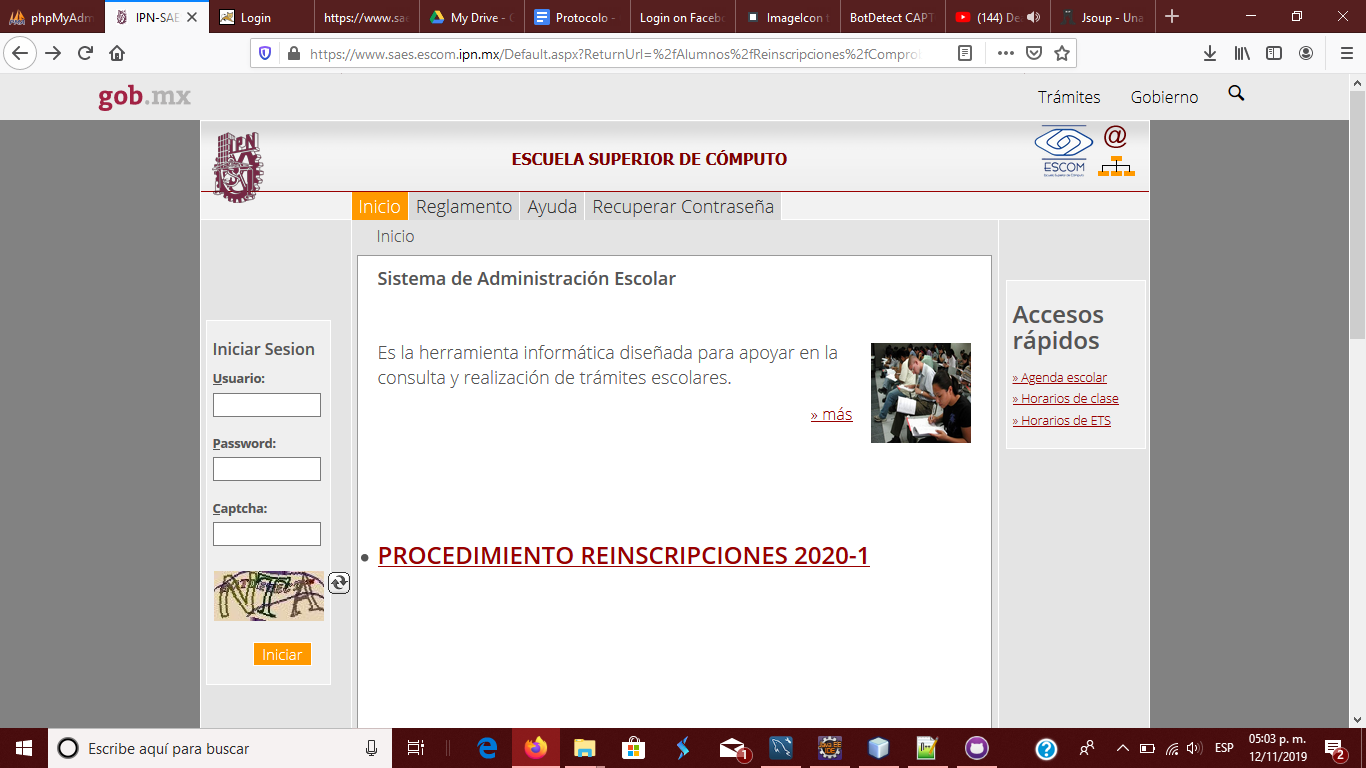
\includegraphics[width=10cm, height=6cm]{Imagenes/Crawler/SAES}
		\caption{Página del SAES Escom}
		\label{saes}
	\end{figure}
	
	\noindent Mediante las herramientas como JSOUP nos permite obtener información del HTML de cualquier página en la web, a excepción de la información generada con javascript pues las obtenciones de información son extraídas de manera estática y no de forma dinámica, o bien desde la lectura del HTML.\\
	\noindent Las pruebas de este código fueron realizadas durante los meses de enero del 2019 y octubre del mismo año. Utilizando así el siguiente código.
	\pagebreak
	
	\noindent Por inicio tenemos que importar las librerías de JSOUP para hacer uso de los métodos que se presentarán a continuación, además de crear datos públicos para los métodos de las clases java para utilizarlos posteriormente.\\
	\noindent Creamos la conexión con la página que queremos explorar y solicitar una respuesta de esta conexión realizada junto con las “cookies” generadas en esta respuesta, ya que estás nos darán pauta para mantenernos en la misma conexión con respecto a la solicitud de conexión hecha anteriormente. \\
	
	\begin{figure} [hbt!]
		\centering
		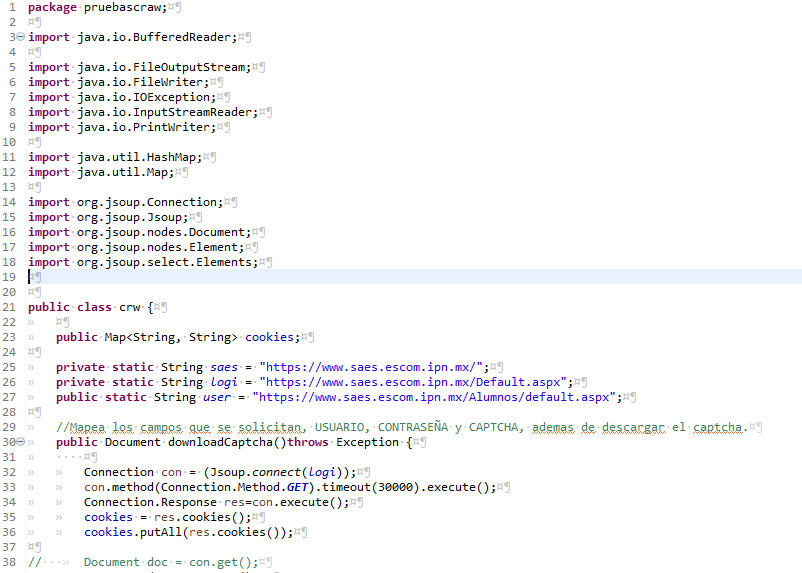
\includegraphics[width=10cm, height=6cm]{Imagenes/Crawler/Codigo1}
		\caption{Código desarrollado implementando el crawler.}
		\label{codigo1}
	\end{figure}
	
	\noindent Lo siguiente es realizar la exploración de los elementos del HTML en una variable de tipo “Document” de la página solicitada donde buscaremos el elemento por ID del CAPTCHA del HTML y así crear una imagen válida que fuese creada por el servidor, extrayendo la ubicación de la imagen para colocarla en una respuesta de conexión con la ruta de la imagen obtenida en la variable “a” y generarla de manera local utilizando “FileOutputStream”, el método creado es de tipo “Document” por lo tanto su salida es del mismo tipo. 
	\pagebreak
	
	\begin{figure} [hbt!]
		\centering
		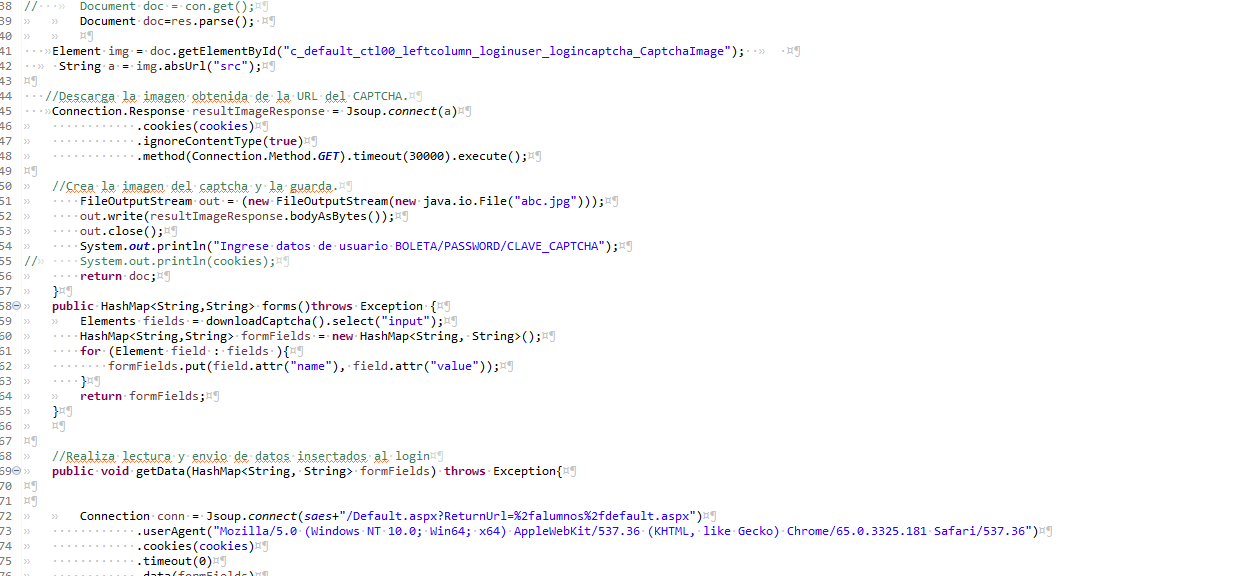
\includegraphics[width=10cm, height=8cm]{Imagenes/Crawler/Codigo2}
		\caption{Continuación de la implementación del crawler.}
		\label{codigo2}
	\end{figure}
	
	\noindent Una vez realizado este método procedemos a explorar los campos de inserción que existen en el HTML, para ello hacemos otra búsqueda de elementos en el HTML y definimos los datos que contienen estos elementos para su posterior inserción y uso de ellos mediante una variable de tipo “HashMap<String,String>” (todos los campos son de tipo cadena).\\
	
	\noindent Ahora la realización del método “getData(HashMap<String,String> formFields)” utilizaremos como parámetros los elementos de inserción explorados anteriormente insertándolos en nuestro método “POST”. Creamos la conexión a donde se debe redirigir la información del inicio de sesión, insertando también las cookies almacenadas en la previa conexión de la obtención del HTML de la página del SAES.\\
	
	\begin{figure} [hbt!]
		\centering
		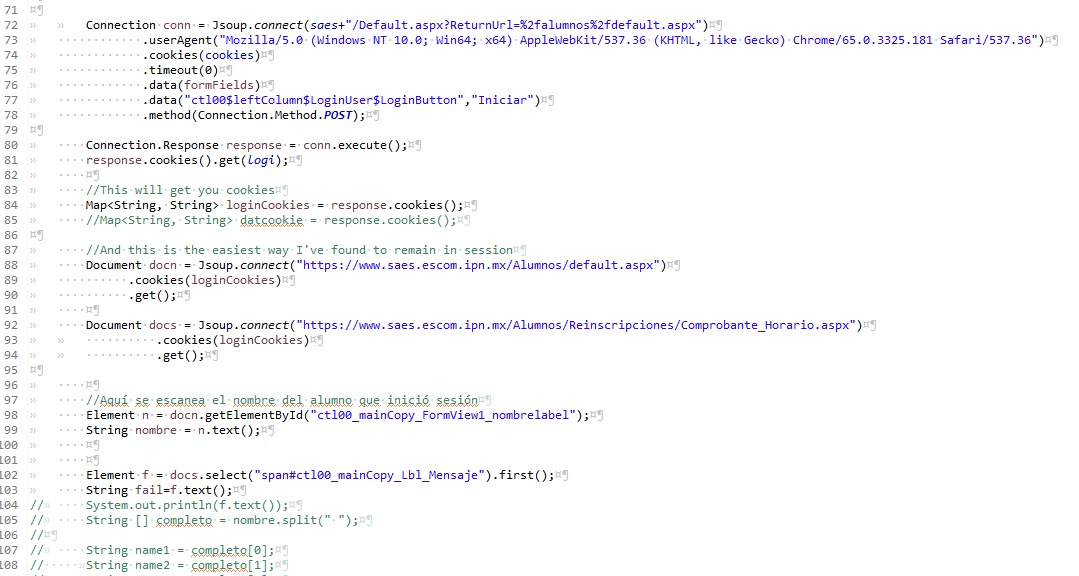
\includegraphics[width=10cm, height=8cm]{Imagenes/Crawler/Codigo3}
		\caption{Continuación implementación del crawler.}
		\label{codigo3}
	\end{figure}
	\pagebreak
	
	\noindent Si los datos ingresados son correctos se realizará una respuesta de la ruta solicitada en el POST insertando las cookies correspondientes a la conexión para comprobar la sesión del usuario en la plataforma, seguido de un mapeo del nuevo HTML donde se realizará la búsqueda por ID del campo donde se encuentre el nombre del alumno y un mensaje donde solo habrá texto si el usuario que haya iniciado sesión no estuviera inscrito.\\
	\noindent De lo anterior y siguiendo la condición de que el usuario que haya iniciado sesión esté o no inscrito dependerá si el texto buscado como “fail” sea nulo/vacío, en el caso de que no lo esté indicará que el alumno que haya iniciado sesión está “INSCRITO” indicando el nombre del alumno que corresponda a la boleta y usuario junto con un grupo al que pertenezca, en el caso de que “fail” no sea nulo/vacío se indicará que el alumno que corresponda a la boleta y usuario aparezca como “NO INSCRITO”. \\
	\begin{figure}[hbt!]
		\centering
		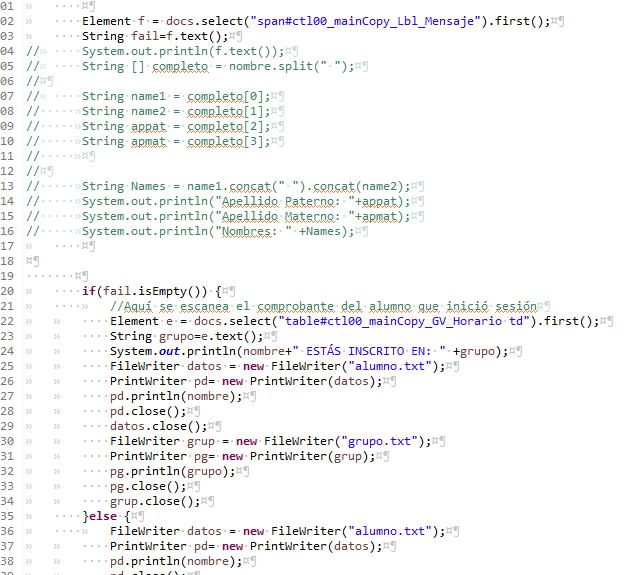
\includegraphics[width=10cm, height=8cm]{Imagenes/Crawler/Codigo4}
		\caption{Continuación implementación del crawler.}
		\label{codigo4}
	\end{figure}
	
	\noindent Finalmente se crean 3 archivos donde se almacena la información del usuario que haya iniciado sesión donde se inserta su nombre completo (alumno.txt), su grupo al que esté inscrito (grupo.txt) y el código HTML de la página donde se obtuvo toda esta información (respoinse.html).
	\pagebreak
	
	\begin{figure}[hbt!]
		\centering
		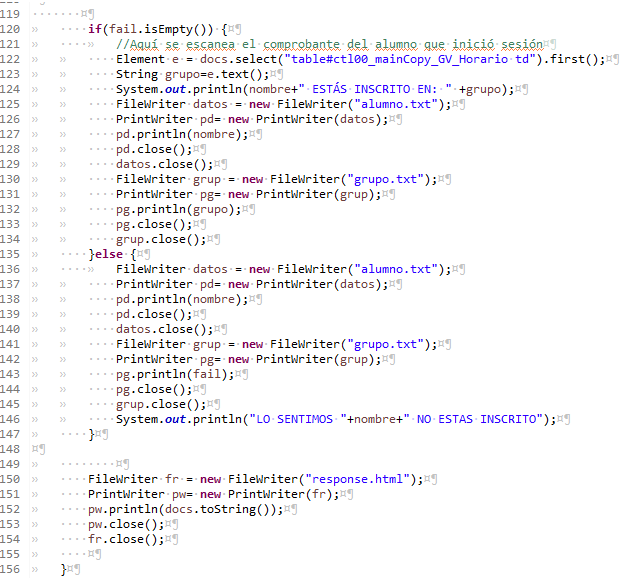
\includegraphics[width=10cm, height=6cm]{Imagenes/Crawler/Codigo5}
		\caption{Continuación de la implementación del crawler.}
		\label{codigo5}
	\end{figure}
	
	\noindent Una vez realizado esto necesitamos adjuntar estos métodos en 1 sola petición (o método) para realizar su ejecución e inserción de datos correspondientes a los que se necesitan.
	Como se hace en el método “run()”. \\
	
	\noindent Creamos un método donde se adjunta en 1 petición la ejecución de todos los métodos anteriores, y haremos la petición de los datos del inicio de sesión del SAES usando “readLine()” para hacer la lectura de estas seguido de la asignación de los campos que se escogen para insertar estas cadenas y reenviarlos al método “getData” donde los datos insertados serán los parámetros que servirán para la correcta funcionalidad del método “getData” y finalmente iniciar sesión.\\
	\begin{figure} [hbt!]
		\centering
		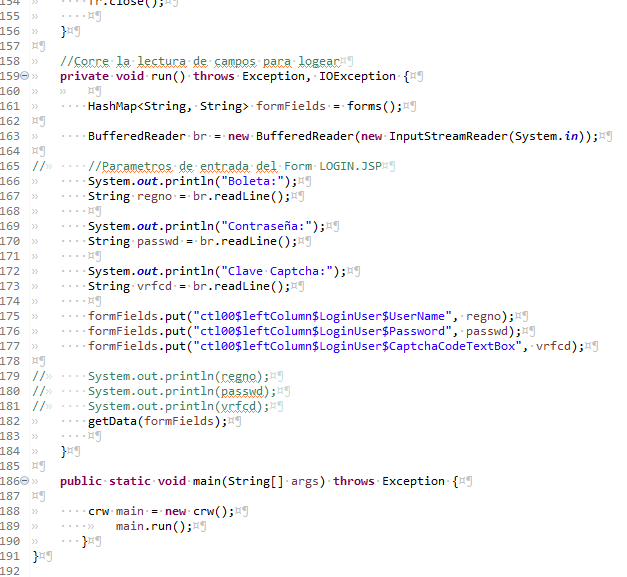
\includegraphics[width=10cm, height=8cm]{Imagenes/Crawler/Codigo6}
		\caption{Continuación implementación crawler.}
		\label{codigo6}
	\end{figure}
	\pagebreak
	\noindent Cabe mencionar que dicha plataforma está desarrollada con ASP.NET con un plugin detector de “bots” llamado “Captcha BotDetect”, donde desde el servidor se realiza la generación de credenciales correspondientes a la imagen que se muestre en la página como la conocemos.\\
	\textbf{“href="BotDetectCaptcha.ashx?get=layoutStyleSheet" ”}\\
	\begin{figure} [hbt!]
		\centering
		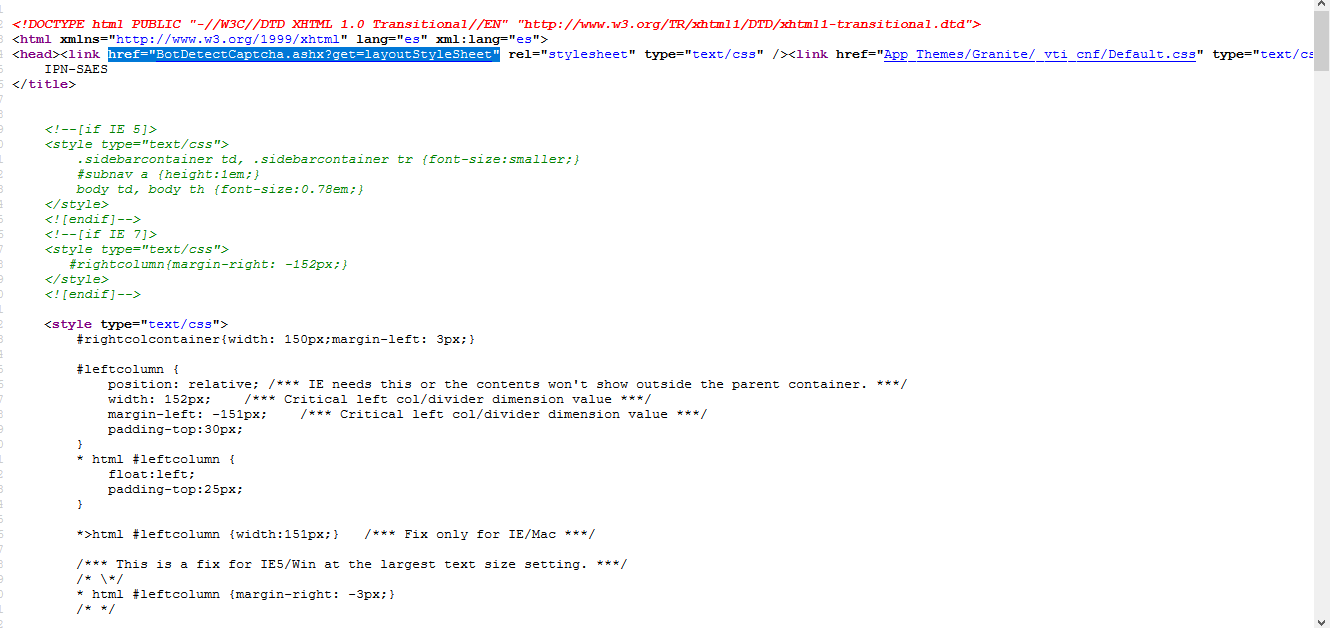
\includegraphics[width=10cm, height=6cm]{Imagenes/Crawler/ASP2}
		\caption{Inspección de estructura del SAES.}
		\label{asp2}
	\end{figure}
	
	\noindent Las peticiones de inicio de sesión se realizan directo al servidor y el servidor responde con un javascript donde redirecciona a la vista correspondiente si las credenciales de usuario y clave captcha son las correctas de acuerdo a la sesión de página en la que se encuentra.\\
	\textbf{“action="Default.aspx?ReturnUrl=\%2fAlumnos\%2fcambia\_clave.aspx" onsubmit="javascript:return WebForm\_OnSubmit();" ”}
	
	\begin{figure} [hbt!]
		\centering
		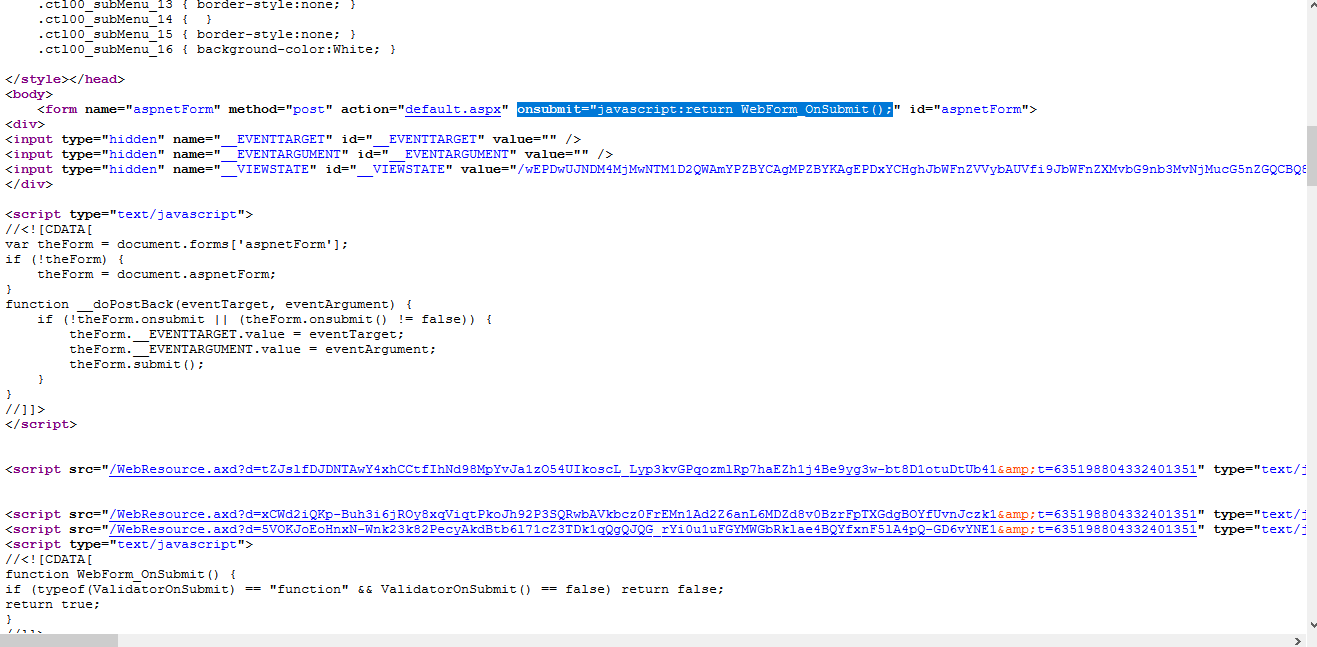
\includegraphics[width=10cm, height=6cm]{Imagenes/Crawler/ASP1}
		\caption{Inspección de estructura del SAES.}
		\label{asp1}
	\end{figure}
	\noindent Estos cambios se identificaron el día 15 de octubre del 2019.
	\pagebreak
	
	\textbf{POR EJEMPLO: CON USUARIO NO INSCRITO}\\
	\noindent Se inserta previamente la boleta y contraseña del alumno del SAES ESCOM.
	
	\begin{figure}[hbt!]
		\centering
		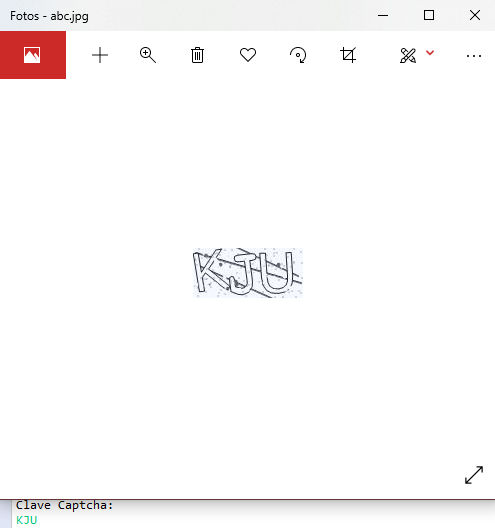
\includegraphics[width=10cm, height=5cm]{Imagenes/Crawler/ImagenloginNoinscrito}
		\caption{Captcha para alumno no inscrito.}
		\label{imagenloginnoinscrito}
	\end{figure}
	
	Se ingresa la clave captcha mostrada en la imagen “KJU”
	
	\begin{figure}[hbt!]
		\centering
		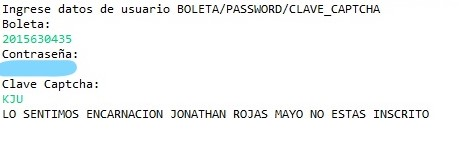
\includegraphics[width=10cm, height=5cm]{Imagenes/Crawler/Datosloginnoinscrito}
		\caption{Se ingresan los datos en el crawler.}
		\label{datosloginnoinscrito}
	\end{figure}
	\noindent Responde de acuerdo a la inscripción del alumno, para este caso el alumno NO ESTÁ INSCRITO.
	\pagebreak
	
	\begin{figure}[hbt!]
		\centering
		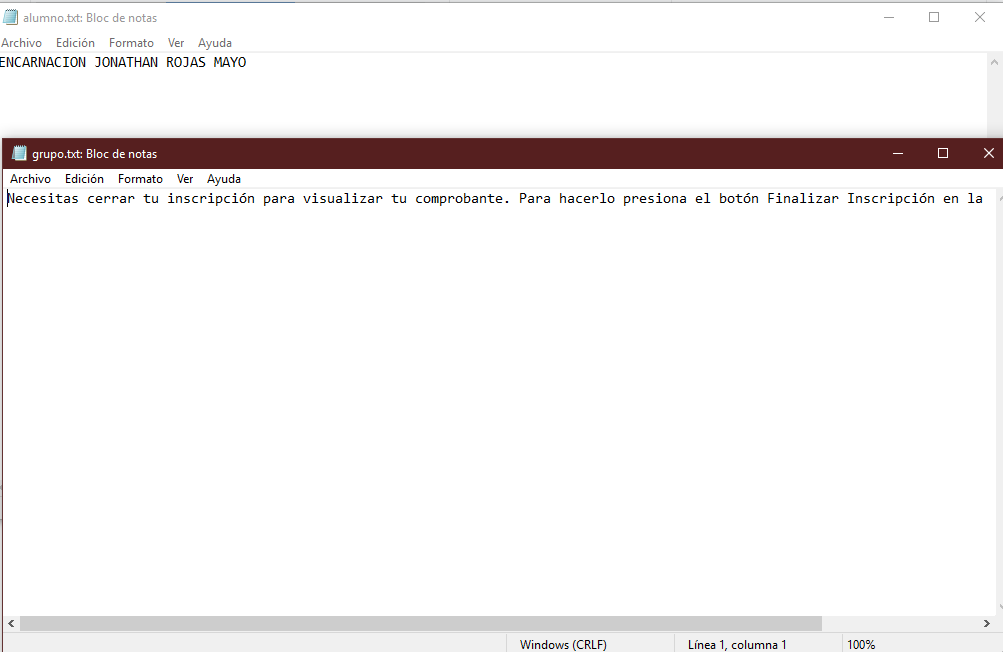
\includegraphics[width=10cm, height=6cm]{Imagenes/Crawler/Noinscrito}
		\caption{Respuesta del crawler.}
		\label{noinscrito}
	\end{figure}
	
	\noindent Se muestran las cadenas correspondientes a la extracción de información para validar que el alumno en cuestión esté inscrito o no lo esté.\\
	
	\textbf{POR EJEMPLO: CON USUARIO INSCRITO}\\
	\noindent Se inserta previamente la boleta y contraseña del alumno del SAES ESCOM.
	
	\begin{figure}[hbt!]
		\centering
		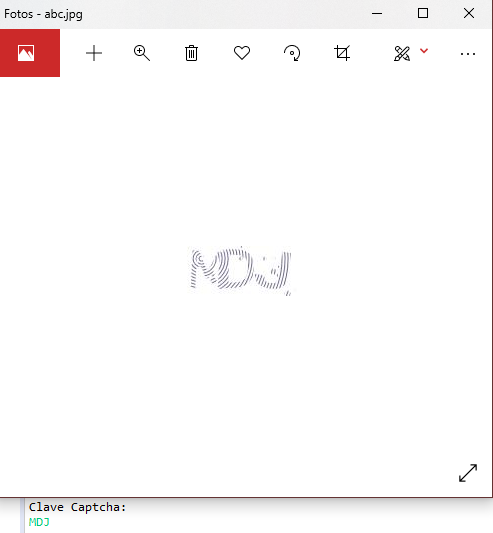
\includegraphics[width=10cm, height=6cm]{Imagenes/Crawler/Imagenlogininscrito}
		\caption{Captcha para el alumno inscrito.}
		\label{imagenlogininscrito}
	\end{figure}
	\noindent Se ingresa la clave captcha mostrada en la imagen “MDJ”
	\pagebreak
	
	\begin{figure}[hbt!]
		\centering
		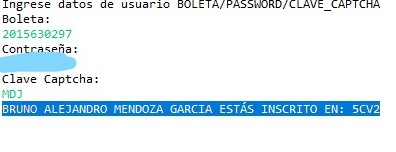
\includegraphics[width=10cm, height=6cm]{Imagenes/Crawler/Datoslogininscrito}
		\caption{Se registran ingresan datos al crawler.}
		\label{datoslogininscrito}
	\end{figure}
	
	\noindent Responde de acuerdo a la inscripción del alumno, para este caso el alumno ESTÁ INSCRITO.
	
	\begin{figure}[hbt!]
		\centering
		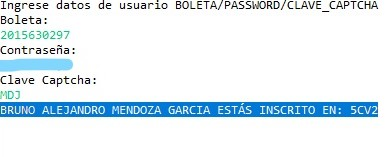
\includegraphics[width=10cm, height=6cm]{Imagenes/Crawler/Logininscrito}
		\caption{Respuesta del crawler.}
		\label{logininscrito}
	\end{figure}
	
	\begin{figure} [hbt!]
		\centering
		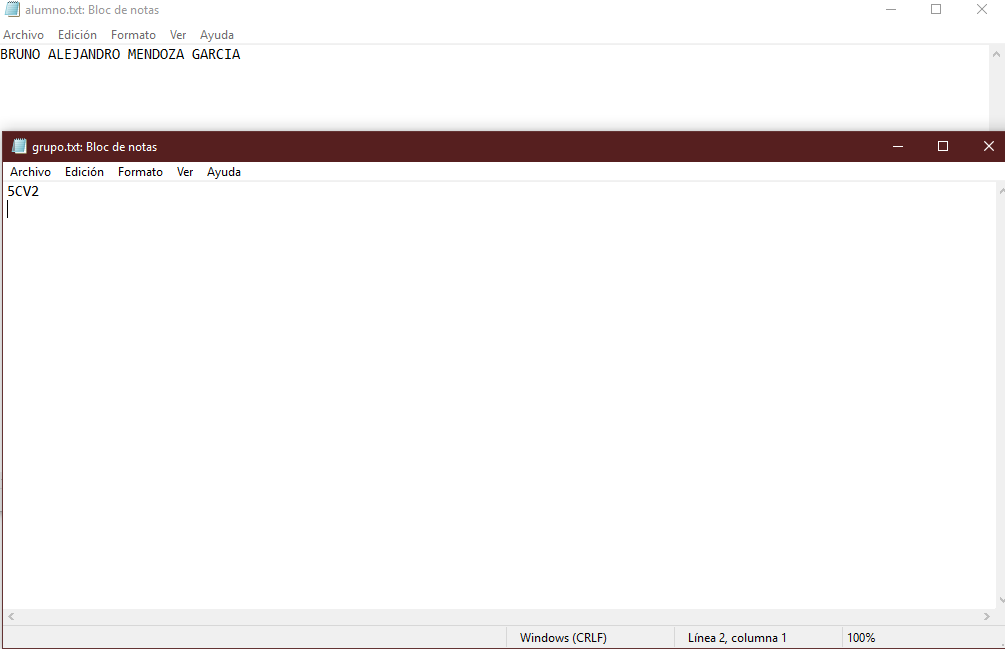
\includegraphics[width=10cm, height=6cm]{Imagenes/Crawler/Infologininscrito}
		\caption{Información del alumno inscrito.}
		\label{infologininscrito}
	\end{figure}
	\noindent Se muestran las cadenas correspondientes a la extracción de información para validar que el alumno en cuestión esté inscrito o no lo esté.
	
	
	%=========================================================
	%              Sistema Gestor de BD del lado del servidor
	%=========================================================
	\section{Sistema Gestor de Base de Datos del lado del servidor}
	\noindent Para persistir la información que se genere a través de la aplicación y que esté disponible la mayor parte del tiempo por los usuarios es necesario contar con un SGBD en el servidor para que los datos están centralizados y se puedan agregar, actualizar, consultar y eliminar los datos generados por los usuarios. Comparando los SGBD, ver la tabla 2, más populares encontramos que la opción más confiable será utilizar MySQL debido a que es de código abierto, gratuito, con soporte técnico y abundante documentación. 
	
	\begin{table}[htbp]
		\begin{center}
			\begin{tabular}{|l|p{35mm}|p{35mm}|p{35mm}|l}
				\hline
				Caracter\'isticas & Oracle & MySQL & SQL Server \\
				\hline 
				Interfaz & GUI, SQL & SQL & GUI, SQL \\ \hline
				Lenguaje soportado & C, C++, C, Java, Ruby y Objective-C & C, C, C++, D, Java, Ruby y Objective C & Java, Ruby, Python, VB, .Net y PHP  \\ \hline
				Sistema Operativo & Windows, GNU/Linux, Solaris, OS-X & Windows, GNU/Linux, OS-X, FreeBSD, Solaris & Windows \\ \hline
				Licencia & Propietrio & Código Libre & Propietario \\ \hline
			\end{tabular}
			\caption{Tabla comparativa de lenguajes de BD.}
			\label{tablaServidor}
		\end{center}
	\end{table}
	
	
	%=========================================================
	%                                                         Servidor
	%=========================================================

	\section{Servidor}
	\noindent Para establecer las caracteristicas de nuestro servidor debemos conocer parte de sus componentes y que operabilidad tendrá dedicada.
	Empezando con los procesadores dedicados para equipos de servidores, se recomienda usar Intel Xeon (cualquier versión), por ejemplo: los servidores con Intel Xeon E5 v3 pueden tener hasta 36 núcleos y se encuentran entre los pocos procesadores que son compatibles con la nueva versión DDR4 de RAM, que utiliza un consumo de energía muy reducido y brinda una excelente velocidad de transferencia de datos.\cite{serv}
	
	\noindent Tomando en cuenta las recomendaciones para armar un buen servidor se tomaron algunas caracteristicas de componentes que pueden ser accesibles para montar el proyecto. \cite{serv}\cite{servi}
	
	\begin{table}[htbp]
		\begin{center}
			\begin{tabular}{|l|l|}
				\hline
				\multicolumn{2}{|c|}{Servidor Ideal} \\
				\hline
				Componentes & \\
				\hline
				\multicolumn{2}{|c|}{Hardware} \\
				\hline
				Procesador & Intel Xeon ó AMD Opteron\\
				\hline
				Plataforma & 64-Bits\\
				\hline
				Memoria RAM & 8 GB\\
				\hline
				Disco Duro & 500 GB\\
				\hline
				Arreglo de Discos Duros & Ninguno\\
				\hline
				Monitor & 800 x 600 16 bits Color o Superior\\
				\hline
				\multicolumn{2}{|c|}{Software} \\
				\hline
				Sistema Operativo & Windows \\
				\hline
				Base de Datos & MySQL 5.1 Community Server\\
				\hline
			\end{tabular}
			\caption{Tabla de especificaciones del servidor.}
		\end{center}
	\end{table}
\pagebreak
\noindent Suponiendo el caso de que por día se hagan 1000 visitas diarias donde se tienen 6 páginas por visita que además por página consume 100kb.

\noindent En condiciones normales, una web envía más datos de los que recibe, por lo cual, hemos de contar con los datos enviados.
\\
\noindent Podremos calcular la transferencia de datos con la siguiente formula\\

(días por mes) x (visitas diarias) x (páginas por visita) x (volumen por página) x 1,25\\

\noindent En cuestión de la memoria RAM está esta pensada de manera que soporte las consultas realizadas por los usuarios en la aplicación, es bien dicho que entre más RAM el servidor tendrá mejor rendimiento \cite{servi}.

\noindent O bien Tomando como caso la capacidad del disco duro se considera que el almacenamiento no se saturará hasta pasado 1 año, puesto que el uso de memoria de almacenamiento de datos creados por la aplicación no serán concurrentes, con el proposito de almacenar la aplicación y los archivos de base de datos, cuya base de datos incrementa de acuerdo al número de usuarios que hagan uso de ella (unicamente los que estén inscritos, o usuarios coordinador).\\


%=========================================================
%                                             Reglas del sistema
%=========================================================
\section{Reglas del Sistema}
\noindent El alumno que desee participar en un evento interpolitécnico hará uso de la aplicación web RIDESCOM. Como primer punto deberá iniciar sesión en la misma, ingresando el usuario y contraseña con el que entra a sistema SAES (Sistema de Administración Escolar). Si los datos ingresados son correctos, se le dará acceso a la aplicación RIDESCOM, en caso contrario no se le dará acceso para poder registrarse en un evento. Sin embargo, podrá seguir visualizando datos generales, como lo es el calendario de eventos, resultados de eventos y los eventos que se practican dentro de la unidad académica.
El Jefe de Fomento Deportivo podrá dar de alta a un Coordinador de alguna Unidad Académica. Para dar de alta un evento deportivo deberá llenar todos los campos requeridos, tendrá la opción de agregar una descripción si así lo desea. 
El Coordinador de la Unidad Académica registrará a los entrenadores de las actividades deportivas deberá llenar los campos requeridos para poder concluir el registro. En caso de que exista un entrenador ya haya sido registrado, la aplicación le notificará. Una vez concluido los eventos deportivos, este registrará los resultados obtenidos por los participantes para que puedan ser vistos por la comunidad en general. 

%=========================================================
%                                             Reglas de Negocio
%=========================================================
\section{Reglas de Negocio}
\noindent La aplicación RIDESCOM permitirá a los alumnos que estén inscritos en el periodo actual, inscribirse en un evento interpolitécnico, consultar los eventos registrados, consultar calendario de eventos. 
El sistema cuenta con una interfaz que nos permite visualizar las diferentes opciones ofrecidas por el mismo. Para acceder al anterior el usuario debe de tener un usuario y contraseña. Dicho usuario y contraseña, será con el que ingresa al sistema del SAES. 
Así mismo, habrá “usuarios encargados”, quienes se encargan de controlar y supervisar el uso de éste ante pequeñas porciones de estudiantes (grupos de alumnos). Ahora dichos encargados hay dos tipos el Jefe de Fomento Deportivo, a este se le permitirá crear eventos deportivos, registrar eventos deportivos y restablecer contraseña a los perfiles de los coordinadores. El segundo tipo de encargado es el Coordinador de una Unidad Académica, este podrá registrar los resultados de los participantes en el sistema para poder ser visualizados en la vista principal, podrá generar un reporte de los alumnos registrados durante el periodo que se haya especificado y registrar a los entrenadores que laboran dentro de la Unidad Académica a la que atienda, a continuación se describirán las reglas para cada uno de los actores que se involucran.
\pagebreak


%=========================================================
%                                             Reglas de Negocio del JFD
%=========================================================
\section{Reglas de Negocio Jefe de Fomento Deportivo}
Para que el JFD pueda ingresar a la página RIDESCOM debe de contar con un Usuario y Contraseña, de caso contrario no podrá acceder.
Una vez dentro de la página de RIDESCOM se le mostrarán las opciones que tiene permitidas, tales como: Evento, Coordinadores, Usuarios, Pruebas en estos dos podrá agregar, editar o eliminar.

\noindent Para la vista de Evento, la información se le mostrará en la página principal, si hay eventos registrados estos serán mostrados en la tabla correspondiente, sino se cuenta con datos se mostrará en la tabla el mensaje de que no existen datos.  Para poder agregar un evento se deben de cumplir con algunos campos que son requisito sino se completan los campos no podrá registrar el evento.  Dentro del formulario para crear el evento se debe asignar una fecha en la que los alumnos podrán inscribirse para esto, no debe de ser mayor  a 5 días en la que se realizará el evento. También se debe considerar que no se puede asignar una fecha menor respecto a la fecha en que se está creando el evento. Una vez tenga el evento registrado podrá editar información respecto a este, teniendo en cuenta los campos que son requisito, o en caso contrario eliminar el evento.

\noindent Para la vista de Coordinadores, se mostrará la información en una tabla dentro de la página principal, en caso de no contar con datos registrados se mostrará un mensaje de que no existen datos. Para poder agregar un Coordinador de Unidad Académica deberá cumplir con campos que son requisitos sino se completan los campos no podrá registrar el coordinador. Una vez tenga el coordinador registrado podrá editar información respecto a este, teniendo en cuenta los campos que son requisito, o en caso contrario eliminar los datos del coordinador.

\noindent Contará con un apartado en el que visualizará los resultados obtenidos por los participantes estos estarán disponibles hasta que concluyan los eventos interpolitécnios y para el JFD solo será de consulta.

\noindent Para la vista de Pruebas, se mostrará una tabla en la que podrá ver las pruebas registradas, en caso de no tener datos que mostrar se mostrará un mensaje en el que se indique que no hay datos por mostrar. Se podrá agregar pruebas, para ello deberá de cumplir con los campos que son requisitos. De igual manera tendrá campos que son requisito para poder guardar los datos. Una vez guardado las Pruebas podrá editar o eliminar la información.

%=========================================================
%                                             Reglas de Negocio del Coord
%=========================================================
\section{Reglas de Negocio Coordinador de Unidad Académica}
\noindent Para que el Coordinador de Unidad Académica pueda ingresar a la página RIDESCOM debe de contar con un Usuario y Contraseña, de caso contrario no podrá acceder.\\

\noindent Una vez dentro de la página de RIDESCOM se le mostrarán las opciones que tiene permitidas, tales como: Constancias, Calendario, Resultados, Consulta Inscritos, DIfundir Evento y Entrenadores. Las vistas antes mencionadas exceptuando Resultados y Difundir Evento, serán vistas de solo lectura.\\

\noindent Para la vista de Constancias el Coordinador de la Unidad Académica podrá consultar si el alumno participó en un evento para que posteriormente, él pueda comenzar el trámite correspondiente para la generación de la constancia. Será solo vista de consulta/lectura. Para la vista de Calendario, se mostrará en la página principal del Coordinador una tabla con los datos que le corresponden, en caso de no tener información se mostrará el mensaje de que no existen datos. Esta vista sólo será de lectura.\\

\noindent Para la vista de Resultados el Coordinador de la Unidad Académica podrá visualizar la información en una tabla dentro de la página principal, en caso de no tener datos se mostrará el mensaje de que no existen datos Para ingresar los resultados obtenidos de los participantes, como el tiempo que se obtuvo, el lugar, etc., deberá de llenar los campos que son requisitos, sino se completan los campos no podrá registrarse el evento. Una vez que se tengan los datos registrados podrá editar o eliminar estos.\\

\noindent Para la vista Difundir Evento, el Coordinador de la Unidad Académica podrá visualizar los eventos que han sido registrados, al selecciona la opción difundir se le mostrará la opción de difundirlo en la red social de facebook.\\

\noindent Para la vista de Entrenadores, se mostrará la información dentro de la vista principal en una tabla, en caso de no contar con información se mostrará el mensaje de que no existen datos. Para agregar datos de un Entrenador se deben de cumplir con datos que son requisitos. Una vez que se tengan datos registrados podrá editar o eliminar la información. \\

\section{Reglas de Negocio Alumno}
Para que el alumno pueda ingresar a la página RIDESCOM debe de contar con un Usuario y Contraseña, de caso contrario no podrá acceder.\\

Una vez dentro de la página de RIDESCOM se le mostrarán las opciones que tiene permitidas, tales como: Calendario, Inscribe Interpolitecnico, Historial,  Resultados, Eventos Inscritos. Las vistas antes mencionadas serán solo lectura exeptuando la vista de INscribe Interpolitecnico.\\

Para la vista de Calendario se mostrará en la página principal en una tabla que contenga la información, en caso de que esta no cuente con información se mostrará el mensaje de que no existen datos. Esta vista sólo será de lectura para el alumno.\\

Para la vista de Inscribir Interpolitecnio, el alumno pueda inscribir un Evento Interpolitecnico deberá como primer punto, validar su status académico, para ello se le mostrará en segunda ocasión el inicio de sesión con esto, se verificará su estatus académico. Si el alumno está inscrito entonces se le mostrará una segundo vista en la que solo será de lectura y verificará si sus datos son correctos. En caso de que el alumno no esté inscrito se le mostrará un mensaje para notificarle que no puede inscribirse dado que no está inscrito en el periodo actual. \\
Si la información que se le presenta es correcta podrá continuar para seleccionar el evento en el que desea participar y así concluir con su inscripción. \\

Para la vista Historial, se mostrará al alumno una tabla que le proporcione información de los eventos en los que ha participado a lo largo de su trayectoria académica. Esta vista es de solo lectura.\\

Para la vista Resultado, se mostrará la información de los resultados del último evento en el que a participado. Esta vista es de solo lectura.\\

Para la vista de Eventos Inscritos, mostrará el o los eventos a los que se a registrado el alumno en el periodo en curso. Esta vista es de solo lectura.\\

\noindent A continuación se mostrarán en distintas tablas las Reglas de Negocio de acuerdo a cada actor que involucra la aplicación.

\begin{table}[hbt!]
	\begin{center}
		\begin{tabular}{|p{30mm}|p{100mm}|}
			\hline
			\multicolumn{2}{|c|}{Jefe de Fomento Deportivo} \\
			\hline
			Identificador & Descripción \\
			\hline 
			RN 1 & Para ingresar a la página debe de contar con un usuario y contraseña. \\ \hline
			RN 2 &  Para registrar un nuevo evento deben de completarse todos los campos que son requisito.\\ \hline
			RN 3 & Para registrar un evento debe de considerar que la fecha de este no sea menor a la fecha en la que se quiere realizar el mismo (no debe de ser mayor  a 5 días en la que se realizará el evento). \\ \hline
			RN 4 &  La fecha de inicio de registro para los alumnos no rebase la fecha en la que se realizará el evento.\\ \hline
			RN 5 &  La fecha de fin de registro para los alumnos no rebase la fecha en la que se realizará el evento. \\ \hline
			RN 6 & Para editar los datos de un evento, no debe de haber alumnos inscritos. \\ \hline
			RN 7 &  Al editar los datos de un evento debe considerar completar todos los campos.\\ \hline
			RN 8 &  Para eliminar un evento, no debe de haber alumnos inscritos en este.\\ \hline
			RN 9 &  Para agregar un deporte, todos los campos que son requisito deben completarse.\\ \hline
			RN 10 &  Al editar un deporte, se debe considerar completar todos los campos requeridos.\\ \hline
			RN 11 &  Para registrar una Prueba, se debe de completar todos los campos.\\ \hline
			RN 12 & Al editar los datos se debe considerar completar todos los campos.\\ \hline
			RN 13 &  Al registrar un nuevo Coordinador, se debe asignar un usuario y contraseña.\\ \hline
			RN 14 &  Para completar el registro, debe completarse todos los campos requeridos.\\ \hline
			RN 15 &  Al editar los datos de un Coordinador, se debe tomar en cuenta completar todos los campos requeridos.\\ \hline
			RN 16 &  Para registrar una Sede, deben completarse todos los campos requeridos.\\ \hline
			RN 17 &  Al editar los datos de una Sede, se debe considerar que esta no esté asignada en un evento.\\ \hline
		\end{tabular}
		\caption{Reglas de Negocio Jefe de Fomento Deportivo.}
		\label{RNJFD}
	\end{center}
\end{table}

\begin{table}[hbt!]
	\begin{center}
		\begin{tabular}{|p{30mm}|p{100mm}|}
			\hline
			\multicolumn{2}{|c|}{Coordinador de Unidad Acedémica} \\
			\hline
			Identificador & Descripción \\
			\hline 
			RN 18 &  Para ingresar a la página debe de contar con un usuario y contraseña.\\ \hline
			RN 19 & Las credenciales deben estar activas y ser proporcionadas por el Jefe de Fomento Deportivo.\\ \hline
			RN 20 & Para ingresar los resultados, debe seleccionar un usuario. \\ \hline
			RN 21 & Se debe seleccionar una prueba correspondiente al alumno.\\ \hline
			RN 22 & Para terminar el proceso de registro de resultados, debe completar los campos requeridos. \\ \hline
			RN 23 & Para registrar un entrenador debe llenar todos los campos requeridos.\\ \hline
			RN 24 & Para obtener la cédula de inscripción, el coordinador deberá de seleccionar el tipo de deporte, así como el ciclo escolar. \\ \hline
			RN 25 & Para consultar si un alumno participó en un evento, se debe buscar por medio de su boleta o por el ciclo escolar en el que participó.\\ \hline
			RN 26 & Para difundir un evento, deberá seleccionar el evento de la tabla y seleccionar el medio por el cual quiere compartir el evento.\\ \hline
		\end{tabular}
		\caption{Reglas de Negocio Coordinador de Unidad Académicas.}
		\label{RNCUA}
	\end{center}
\end{table}

\pagebreak

\begin{table}[hbt!]
	\begin{center}
		\begin{tabular}{|p{30mm}|p{100mm}|}
			\hline
			\multicolumn{2}{|c|}{Alumno} \\ \hline
			Identificador & Descripción \\ \hline 
			RN & Para ingresar a la página debe de contar con un usuario y contraseña.\\ \hline
			RN & El alumno debe verificar el estatus académico para poder registrarse en un evento.\\ \hline
			RN & Para concluir el registro al evento, debe de llenar todos los campos requeridos.\\ \hline
			RN & Puede inscribirse en los eventos que desee, siempre y cuando no tenga traslape en horas de los eventos.\\ \hline
			RN & \\ \hline
			RN & \\ \hline
		\end{tabular}
		\caption{Reglas de Negocio para el alumno.}
		\label{RNA}
	\end{center}
\end{table}
\pagebreak

%=========================================================
%                                                         Requisitos de interaccion con el usuario
%=========================================================
\section{Requisitos del usuario}
A continuación se mostrarán los requisitos indispensables que se deben considerar para el usuario, así como la prioridad de cada uno de ellos. Estos servirán para el desarrollo de los módulos que conformarán la aplicaciónweb 
\begin{table}[htbp]
	\begin{center}
		\begin{tabular}{|l|p{45mm}|p{45mm}|p{45mm}|l}
			\hline
			Id & Nombre & Descripción & Prioridad \\
			\hline 
			RF1 & Registro de eventos & En la aplicación web se podrán registrar, modificar, eliminar y consultar  en un formulario todos los datos para identificar un evento.
			& MEDIA \\ \hline
			RF2 & Registro de participantes & En la aplicación web se podrán registrar, modificar, eliminar y consultar  en un formulario los datos del participante & ALTA  \\ \hline
			RF3 & Vista al público & En una pantalla se mostrarán los participantes que estén registrados en la aplicación y ver sus resultados de competencia. & MEDIO \\ \hline
			RF4 & Conexión con red social FACEBOOK. & Gracias a los datos que identifican a un evento se podrá promover en la red social FACEBOOK mediante el uso de API.& ALTA \\ \hline
			RF5 & Realizar una interfaz para los participantes (alumnos). &Se creará un(una ventana)  sitio para los alumnos que quieran participar en algún evento deportivo(, haciendo su registro, consultar estatus). & MEDIA \\ \hline
			RF6 & Mostrar una tabla de estadísticas. & En una pantalla (vista)  se mostrará todas las áreas deportivas que participaron en el evento deportivo y  número de participantes. & ALTA \\ \hline
			RF7 & Registrar un coordinador & El coordinador que utilizará la aplicación web tendrá que ser registrado en la base de datos. & ALTA \\ \hline
			RF8 & Vista para el coordinador. &El coordinador tendrá una vista donde podrá dar de alta eventos, participantes y generar cédulas de inscripción. & MEDIA \\ \hline
			RF9  & Historial & Para que se tenga un monitoreo de participantes. & ALTA \\ \hline
		\end{tabular}
		\caption{Requerimientos del Usuario.}
		\label{tabla:sencilla}
	\end{center}
\end{table}
\pagebreak

%=========================================================
%                                                         Requisitos funcionales
%=========================================================
\section{Requisitos funcionales de la aplicación web}
En la tabla mostrada a continuación, se muestrán los requisitos funcionales de la aplicación web los cuales serviran para el desarrollo de la aplicación web, así como la prioridad de cada uno de ellos.
\pagebreak
\begin{table}[htbp]
	\begin{center}
		\begin{tabular}{|l|p{45mm}|p{45mm}|p{45mm}|l}
			\hline
			Id & Nombre & Descripción & Prioridad \\
			\hline 
			RF1 & Conexión a internet. & La aplicación deberá estar siempre conectada a internet & ALTA \\ \hline
			RF2 & Validación de datos de los participantes. & La aplicación contará con un mecanismo de comprobación de estado académico (inscrito). & ALTA \\ \hline
			RF3 & Historial de participante. & Para tener seguimiento del participante durante su trayectoria académica & MEDIA  \\ \hline
			RF4 & Comunicación con la red social FACEBOOK &Habrá comunicación con la red social FACEBOOK para la publicación de eventos registrados en la aplicación.  & MEDIO \\ \hline
			RF5 & Creación de perfiles. & Se podrá asignar un perfil a un usuario.& MEDIA \\ \hline
		\end{tabular}
		\pagebreak
		\caption{Requerimientos funcionales de la aplicación web.}
		\label{requisitosFuncionales}
	\end{center}
\end{table}


%=========================================================
%                                                         Requisitos de informacion
%=========================================================
\section{Requisitos no funcionales de la aplicación web}
En la tabla mostrada a continuación se muestran los requisitos que no afectan al funcionamiento de la aplicación, sin embargo se consideran para que en caso de tener el tiempo, se integran a la aplicación y obtener un complemento al resultado fijado.
\begin{table}[htbp]
	\begin{center}
		\begin{tabular}{|l|p{45mm}|p{45mm}|p{45mm}|l}
			\hline
			Id & Nombre & Descripción & Prioridad \\
			\hline 
			RF1 & Vista de consulta genera. & Comunidad ajena a los participantes podrán ver los resultados. & MEDIA \\ \hline
			RF2 & Lista de registros &El usuario podrá consultar sus registros realizados & MEDIA   \\ \hline
			RF3 & Recuperación de contraseña &El usuario participante podrá recuperar su contraseña. & MEDIO \\ \hline
		\end{tabular}
		\caption{Requerimientos no funcionales de la aplicación web.}
		\label{tabla:sencilla}
	\end{center}
\end{table}
\pagebreak

%=========================================================
%                                    Diagrama de procesos
%=========================================================
\section{Diagrama de Procesos}
\noindent En este apartado se explicará y detallará el proceso actual que sigue el alumno para poder registrarse en un evento interpolitécnico deportivo, posteriormente se hace mención del proceso porpuesto para el mismo fin.\\
El proceso actual que el alumno debe seguir para inscribirse a un evento interpolitécnico deportivo comienza cuando el alumno acude al Deportamento de Actividades Deportivas de su unidad académica donde el encargado del departamento le proporciona un formato el cual debe llenar a mano. Este formato se debe de llenar de acuerdo al número de eventos en el que el alumno quiera participar.\\
El formato antes mencionado solicita campos como: nombre, deporte, escuela, prueba, entre otros. Una vez completado el formato el alumno entrega su solicitud al encargado del Departamento y este hace mención que se comunicarán con el en cuanto se tenga una actualización acerca de su solicitud.\\
\noindent El proceso continua con el encargado del Departamento de Actividades Deportivas quien genera una lista de alumnos solicitantes para posteriormente comprobar su estatus académico. Esto se realiza ya que según el reglamento solo los alumnos participantes son los que pueden participar en los eventos.
Una vez que realizada la comprobación se le notifica al alumno el estatus final de su solicitud, sea aceptada o rechazada.
El coordinador de la unidad académica realiza un listado con los alumnos que participaran en los eventos de acuerdo al ciclo escolar en curso para que sea enviado al Departamento de Fomento Deportivo.
Finalmente el alumno espera a que sea la fecha del evento para hacer su participación. Una vez concluido estos, se procede a pagar el arbitraje que se contrata para llevar control de las actividades deportivas.\\
\noindent Una vez pagado el arbitraje se pasa a hacer el llenado de los resultados obtenidos para cada uno de los participantes para así ser publicados y pueda ser visualizados por la comunidad estudiantil.


%=========================================================
%                                                         Reglas de Negocio del Sistema
%=========================================================
%\section{Reglas de necocio de la aplicación}


\section{Diseño de pantallas}}
\noindent Las vistas han cambiado conforme avanza el proyecto, en este caso, se han omitido unas vistas ya que durante nuestra investigación para implementar el registro a la página RIDESCOM para los alumnos, en un inicio se planteo hacer una conexión con la base de datos de la Dirección de Administración Escolera (DAE) para poder verificar que sus datos sean reales. Este método de comprobación iba a ser difícil de llevar a cabo ya que por el hecho de manejar datos sensibles no se nos podía ser brindada. Por esta razón se investigo como poder implementar un crawler, que se conecta con el SAES. Dentro de la página RIDESCOM se solicitan los mismos campos que en el SAES: Usuario, Contraseña y Captcha, si los datos que se ingresaron son correctos el alumno podrá ingresar a RIDESCOM, en caso contrario se le notificará que los datos son erróneos. \\
Las vistas que se eliminaron son las siguientes: 

\begin{figure}[hbt!]
	\centering
	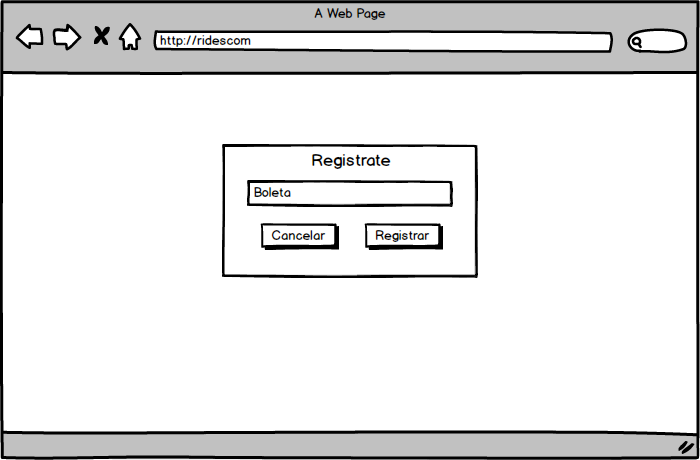
\includegraphics[width=10cm, height=6cm]{Imagenes/Disenos/VistasBorradas/p1_Registro.png}
	\caption{Registro para los alumnos.}
\end{figure}

\begin{figure}[hbt!]
	\centering
	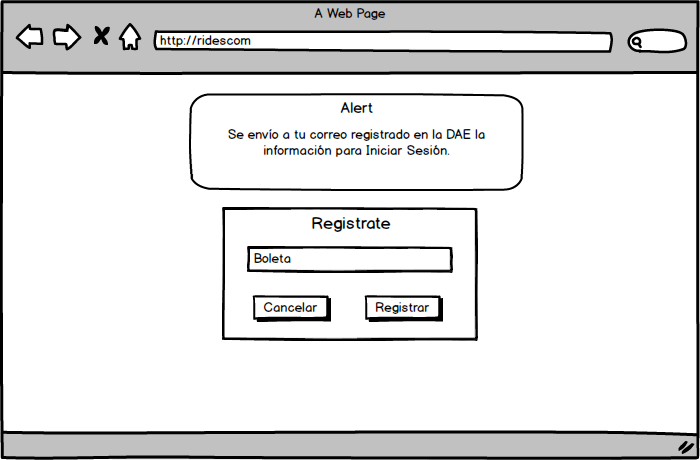
\includegraphics[width=10cm, height=6cm]{Imagenes/Disenos/VistasBorradas/ConfirmacionRegistro.png}
	\caption{Confirmación registro para los alumnos.}
\end{figure}

\begin{figure}[hbt!]
	\centering
	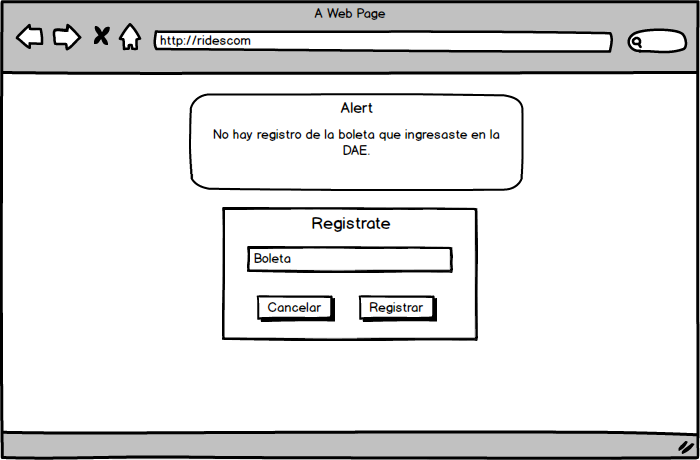
\includegraphics[width=10cm, height=6cm]{Imagenes/Disenos/VistasBorradas/p3RechazoRegistro.png}
	\caption{Rechazo registro para los alumnos.}
\end{figure}

\begin{figure}[hbt!]
	\centering
	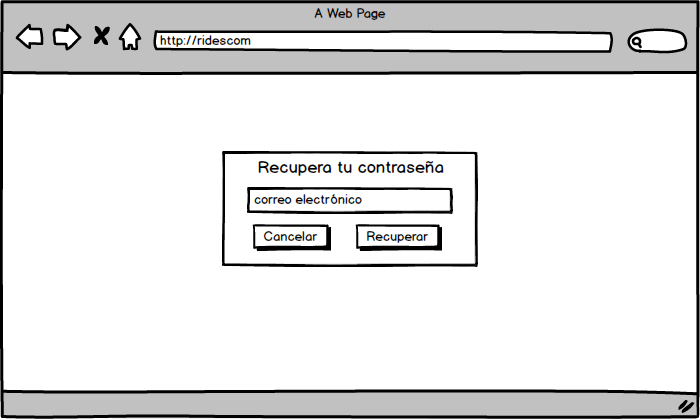
\includegraphics[width=10cm, height=6cm]{Imagenes/Disenos/VistasBorradas/p5Recuperarcontrasena.png}
	\caption{Recuperar contraseña para los alumnos.}
\end{figure}

\begin{figure}[hbt!]
	\centering
	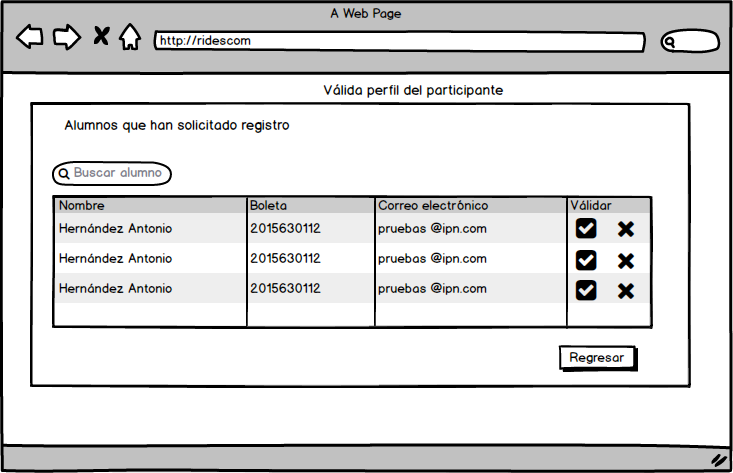
\includegraphics[width=10cm, height=6cm]{Imagenes/Disenos/VistasBorradas/p18ValidaPerfil.png}
	\caption{Validar perfil de los alumnos.}
\end{figure}
\pagebreak


	\newpage
	%=========================================================
	%                                                         Capitulo 4 Análisis
	%=========================================================
		\chapter{Prototipo RIDESCOM}

	\noindent En este capítulo se presenta un resumen del trabajo realizado durante el periodo correspondiente a Trabajo Terminal 1, esto servirá como base para entender los procesos y el desarrollo correspondiente a Trabajo Terminal 2.\\
	\noindent Siendo así se presentará el plan de trabajo establecido para Trabajo Terminal 2 de tal manera que posteriormente, pueda explicarse a detalle los logros obtenidos, incluyendo las problemáticas y la solución a estos. \\
	
	%=========================================================
	%                                                     Antecedentes
	%=========================================================
	\section{Introduccción}
	\noindent Durante el periodo correspondiente al Trabajo Terminal 1, de acuerdo al calendario de actividades, se realizó la toma de requerimientos para delimitar el alcance del proyecto. Una vez realizado esto, se procedió a realizar el análisis del proyecto identificando los módulos que ayudarían a mitigar la problemática y a su vez estos sean fácil de usar. Se tuvo una constante comunicación con el Jefe de Fomento Deportivo quien daba la decisión final de las vistas así como la usabilidad de los mismos.\\
	
	\noindent Se diseño la base de datos, la tiene el soporte para manejar todas las unidades académicas que conforman al IPN, independientemente que para el Trabajo Terminal se tomó como caso de estudio a la ESCOM. Se planteó el diseño de las pantallas que contaría la aplicación web.\\
	
	\noindent Un punto importante del Trabajo Terminal 1 fue la implementación de un Crawler, el cual ayudará a atacar dos de los principales problemas existentes. Uno de ellos es que el alumno interesado en participar en un evento interpolitécnicos sea estudiante del IPN. El segundo problema es la participación de alumnos que no están inscritos en el ciclo escolar en el cual se quiere participar.
	
	\section{Plan de trabajo}
	\noindent A continuación se muestra el cronograma correspondiente a Trabajo Terminal 2 este servirá para explicar detalladamente el trabajo en cada uno de los Sprint, los problemas y las soluciones a estos.
	\begin{figure}[hbt!]
		\centering
		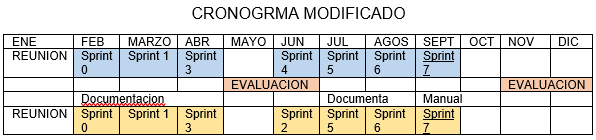
\includegraphics[width=13cm, height=4cm]{Imagenes/cronograma}
		\caption{Cronograma de actividades correspondientes a Trabajo Terminal 2}
		\label{cronograma}
	\end{figure}
\pagebreak

	\noindent Para tener el contexto de los casos de uso involucrados encada usuario que interactua con la aplicación web corresponde a la Figura \ref{diagramaCU}.
	\begin{figure}[hbt!]
		\centering
		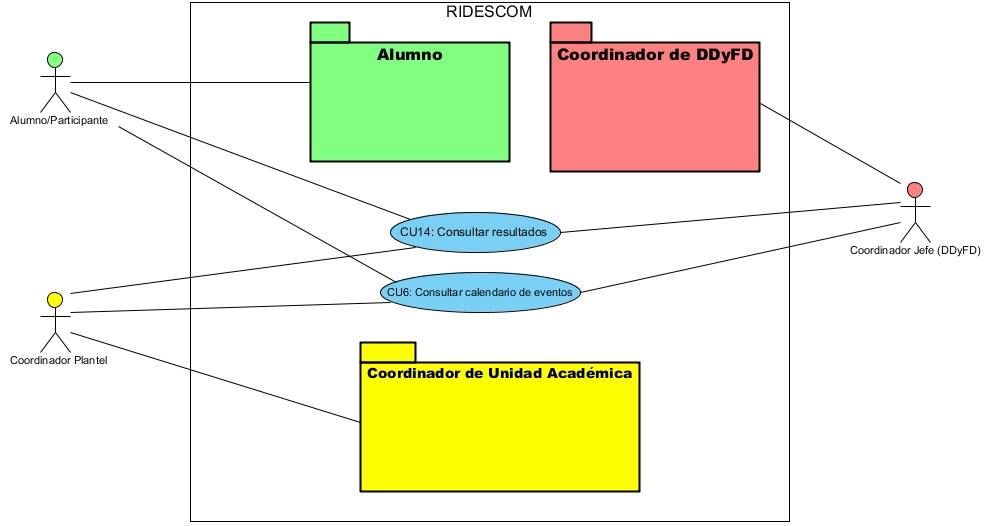
\includegraphics[width=10cm, height=6cm]{Imagenes/diagramaCU}
		\caption{Diagrama de clase de uso.}
		\label{diagramaCU}
	\end{figure}

	\noindent De tal manera que pueda ser más fácil y entendible, se desglozaron los casos de uso en cada actor. Teniendo como primer punto el diagrama correspondiente al Jefe de Fomento Deportivo, seguido del diagrama del coordinador de unidad académica, finalmente se tiene el diagrama del alumno, como se muestra en las Figuras \ref{diagramacujfd}, \ref{diagramacucoord} y \ref{diagramacualumno}.
	
	\begin{figure} [hbt!]
		\centering
		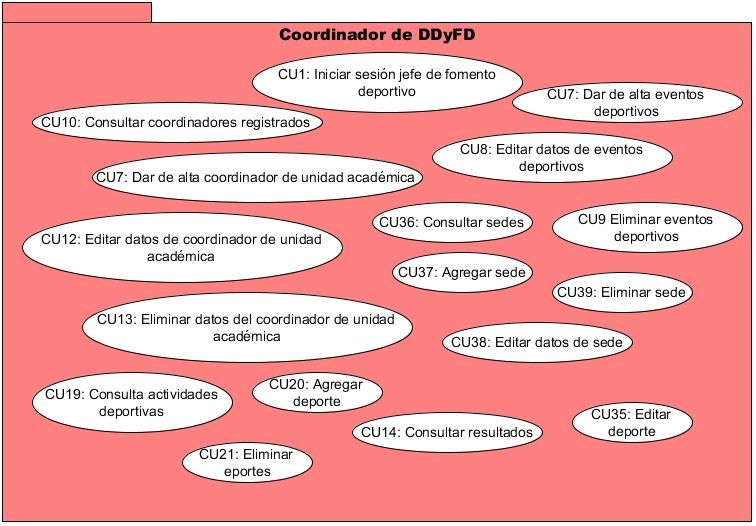
\includegraphics[width=10cm, height=6cm]{Imagenes/diagramaCUJFD}
		\caption{Diagrama de casos de uso del Jefe de Fomento Deportivo.}
		\label{diagramacujfd}
	\end{figure}
\pagebreak
	
	\begin{figure}[hbt!]
		\centering
		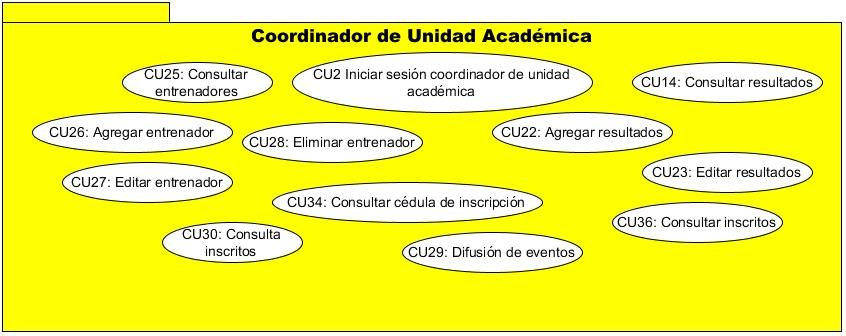
\includegraphics[width=10cm, height=6cm]{Imagenes/diagramaCUCoord}
		\caption{Diagrama de casos de uso del coordinador de unidad académica}
		\label{diagramacucoord}
	\end{figure}

	\begin{figure} [hbt!]
		\centering
		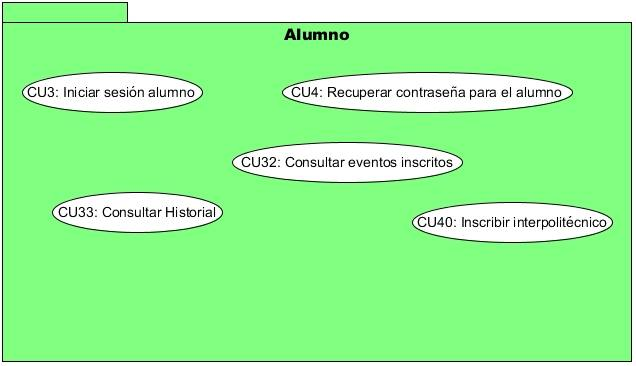
\includegraphics[width=10cm, height=6cm]{Imagenes/diagramaCUAlumno}
		\caption{Diagrama de casos de uso para el alumno}
		\label{diagramacualumno}
	\end{figure}
	
	
	

	\noindent Ahora bien, los Sprint a desarrollar son: 
	\begin{itemize}
		\item Sprint 2
		\item Sprint 4
		\item Sprint 5
		\item Sprint 6
		\item Sprint 7
	\end{itemize}
	\noindent En este capítulo se muestran las iteraciones que realizamos los primeros 4 meses del año 2019 siguiendo la metodología Scrum. En las primeras iteraciones se realizó la investigación acerca de los aspectos fundamentales de las páginas web, con el fin de comprender los conceptos del desarrollo de aplicaciones y poder llevarlos a la práctica. En iteraciones posteriores se hizo un análisis de lo que va a realizar RIDESCOM; de ese análisis se obtuvieron los requisitos funcionales y no funcionales del sistema, una breve descripción de los casos de uso, así como la identificación de los actores, se fueron obteniendo reglas de negocio. Además, de seguir con la investigación y práctica de la creación de aplicaciones web y del uso o implementación de un crawler. Posteriormente se comenzó con la redacción de la documentación técnica, la investigación del estado del arte, el análisis y diseño de la base de datos, la comprensión de comandos de LaTeX, el diseño que tendrá la aplicación, se realizaron pantallas de como lucirá la apliación, se definieron los iconos que se utilizarán en la aplicación, se definieron las tecnologías a utilizar, se implementó un servidor local para la interacción con la aplicación móvil, se creó un primer prototipo de la aplicación con la vista del crawler (Inicio Sesión) y se realizó la redacción de este documento que es el reporte de actividades realizadas. También se creó el repositorio para el desarrollo colaborativo de los documentos. En estas iteraciones surgieron problemas e inconvenientes que afectan al proyecto RIDESCOM tales como la implementación de un crawler, la curva de aprendizaje del desarrollo utilizando Spring MVC, las limitaciones de tiempo debido a que los miembros del equipo trabajan o están realizando su servicio social. Pese a los problemas mencionados o no, tenemos un prototipo funcional de la aplicación así como la mayor parte de la documentación técnica y la elaboración de este documento. El resto de este capítulo presenta en mayor o menor medida los detalles del trabajo realizado en cada iteración. A continuación se explicara a detalle el trabajo realizado en cada uno de los Sprint antes mencionados.

	
	\section{An\'alisis de factibilidad t\'ecnica}
	\noindent Éste análisis tiene como objetivo describir las herramientas que pueden ocuparse para la realización de este proyecto mencionando sus objetivos de cada herramienta de trabajo seleccionada.
	
	\begin{table}[htbp]
		\begin{center}
			\begin{tabular}{|p{20mm}|p{30mm}|p{15mm}|p{15mm}|p{15mm}|}
				\hline
				\textbf{Puesto} & \textbf{Descripción de actividades} & \textbf{Salario mensual} & \textbf{Cantidad} & \textbf{Total por mes}\\ \hline 
				Project Manager Analista & Encargado de supervisar el desarrollo del sistema y participará en el desarrollo del mismo & 17,00 MXN. & 1 &17,00 MXN. \\ \hline
				
				Programador Back-end & Encargado de desarrollar la parte lógica del proyecto & 12,500 MXN. & 1 &12,500 MXN. \\ \hline
				
				Programador Front-end & Encargado de desarrollar las interfaces del proyecto & 12,500 MXN. & 1 &12,500 MXN.\\ \hline
				
				\multicolumn{4}{|c|}{Total por el desarrollo del sistema: 10 meses} & 420,000 MXN.\\ \hline
			\end{tabular}
			\caption{Tabla de costos del personal.}
			\label{tablacostopersonal}
		\end{center}
	\end{table}
	
	\begin{table}[htbp]
		\begin{center}
			\begin{tabular}{|p{20mm}|p{30mm}|p{15mm}|p{15mm}|}
				\hline
				\textbf{Servicio}  & \textbf{Características} & \textbf{Precio mensual} & \textbf{Total} \\ \hline 
				Paquete esencial de TotalPlay & Telefonía ilimitada Intenet de 50 MG. & 459 MXN. & 5,049 MXN \\ \hline
				
				Luz & - & Varía de acuerdo a las tarifas establecidas por CFE & 2,354 MXN. \\ \hline
				
				\multicolumn{3}{|c|}{Total por el desarrollo del sistema: 10 meses} & 7,403 MXN\\ \hline
			\end{tabular}
			\caption{Tabla de costos operativos.}
			\label{tablacostosoperativos}
		\end{center}
	\end{table}
\pagebreak
	
	\begin{table}[htbp]
		\begin{center}
			\begin{tabular}{|p{20mm}|p{30mm}|p{15mm}|p{15mm}|p{15mm}|}
				\hline
				\textbf{Equipo} & \textbf{Características} & \textbf{Cantidad} & \textbf{Unidad} & \textbf{Precio}\\ \hline 
				Laptop HP Pavilion & Procesador AMD 5, Memoria RAM: 8 GB, Disco duro: 512GB, Sistema operativo: Windows 10  & 1 & Pieza & 15,00 MXN. \\ \hline
				
				Laptop HP Pavilion & Procesador AMD 5, Memoria RAM: 8 GB, Disco duro: 512GB, Sistema operativo: Windows 10  & 1 & Pieza & 15,00 MXN. \\ \hline
				
				\multicolumn{4}{|c|}{Total por el desarrollo del sistema: 10 meses} & 30,000 MXN.\\ \hline
			\end{tabular}
			\caption{Tabla de costos de herramientas de desarrollo.}
			\label{tablcostoherramientas}
		\end{center}
	\end{table}
	
	\begin{table}[htbp]
		\begin{center}
			\begin{tabular}{|p{20mm}|p{30mm}|p{15mm}|p{15mm}|p{15mm}|}
				\hline
				\textbf{Producto} & \textbf{Cantidad} & \textbf{Unidad} & \textbf{Precio}  & \textbf{Precio Total}\\ \hline 
				Paquete de 100 hojas blancas & 1  & Pieza & 22.50 MXN. & 22.50 MXN. \\ \hline
				
				Engargolado & 2 & - & 22 MXN. & 44 MXN. \\ \hline
				
				CD virgen & 2 & Pieza & 8 MXN. & 16 MXN. \\ \hline
				
				Impresiones & 200 & - & 0.32 MXN. & 64 MXN \\ \hline
				
				\multicolumn{4}{|c|}{Total por el desarrollo del sistema: 10 meses} & 30,000 MXN.\\ \hline
			\end{tabular}
			\caption{Tabla de costos de herramientas de papelería.}
			\label{tablacostospapeleria}
		\end{center}
	\end{table}
\pagebreak
	
	\begin{table}[htbp]
		\begin{center}
			\begin{tabular}{|p{20mm}|p{30mm}|p{15mm}|p{15mm}|}
				\hline
				\textbf{Fase de desarrollo}  & \textbf{Horas requeridas} & \textbf{Total de días empleados} & \textbf{Total} \\ \hline 
				Análisis, diseño y planeación & 4 & 150 & 600 \\ \hline
				
				Desarrollo, implementación y pruebas & 6 & 180 & 1080 \\ \hline
				
				\multicolumn{3}{|c|}{Total de horas requeridas} & 1680\\ \hline
			\end{tabular}
			\caption{Tabla de costo de tiempo de desarrollo.}
			\label{tablacostodesarrollo}
		\end{center}
	\end{table}
	
	\noindent El Modelo Básico de COCOMO’81 estima el esfuerzo y el tiempo empleado en el desarrollo
	de un proyecto de software usando dos variables predictivas denominadas factores de costo (cost
	drivers): el tamaño del software y el modo de desarrollo. Las ecuaciones básicas son: \\
	\textbf{Esfuerzo:}
	$PM = A * (KSLOC)^{B} $\\
	
	\noindent Donde: 
	\begin{itemize}
		\item PM: Es el esfuerzo estimado. Representa los meses-persona necesarios para ejecutar el proyecto.
		\item KSLOC: Es el tamaño del software a desarrollar en miles de líneas de código.
		\item A y B: son coeficientes que varían según el Modo de Desarrollo (Orgánico, Semiacoplado, Empotrado).
	\end{itemize}
	
	\textbf{Cronograma:}
	$TDEV = C * (PM)^{D} $\\
	\noindent Donde: 
	\begin{itemize}
		\item TDEV: Representa los meses de trabajo que se necesitan para ejecutar el proyecto.
		\item C y D: son coeficientes que varían según el Modo de Desarrollo (Orgánico, Semiacoplado, Empotrado).
	\end{itemize}
	
	\noindent Tomando en cuenta las formulas anteriores se completa la tabla siguiente:
	
	\begin{table}[htbp]
		\begin{center}
			\begin{tabular}{|p{20mm}|p{45mm}|p{45mm}|}
				\hline
				\textbf{Modo de desarrollo}  & \textbf{Esfuerzo} & \textbf{Cronograma} \\ \hline 
				Orgánico & $ PM = 2.4 * (KSLOC)^{1.05}$  PM = 50 & $ TDEV = 2.5 * (PM)^{0.38}$  \\ \hline
				
				Semiacoplado & $ PM = 2.4 * (KSLOC)^{1.12}$ & $ TDEV = 2.5 * (PM)^{0.35}$  \\ \hline
				
				Empotrado & $ PM = 2.4 * (KSLOC)^{1.20}$ & $ TDEV = 2.5 * (PM)^{0.32}$  \\ \hline
			\end{tabular}
			\caption{Tabla de costo de tiempo de desarrollo.}
			\label{tablacocomo}
		\end{center}
	\end{table}
	
	
	%=========================================================
	%                                                         Sprint 2
	%=========================================================
	\section{Sprint 2: Interfaces}
	\noindent Para la desarrollo de este SPRINT se tomaron los debidos requerimientos para la realización del diseño de las interfaces y así hacer que la aplicación sea amigable con el usuario utilizando las siguientes plantillas para la visualización de las interfaces como una propuesta.
	\newline
	
	\noindent Interfaz Inicio general: Esta interfaz es la principal donde los usuarios podrán visualizar datos de aspecto público. 
	\newline
	Parte 1:
	Cualquier usuario que visite la URL de la aplicación podrá ver los elementos de navegación tales como: Inicio (Página principal), Registro, Calendario, Inicia Sesión, Contacto, los deportes que se imparten en la ESCOM, una introducción a los eventos interpolitécnicos deportivos próximos, como se muestra en la Figura \ref{inicioGeneral}. 
	\newline
	\begin{figure}[hbt!]
		\centering
		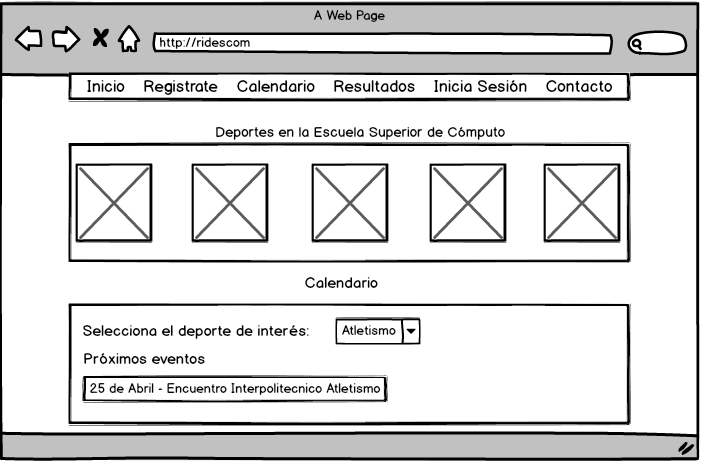
\includegraphics[width=10cm, height=6cm]{Imagenes/Disenos/Iniciogeneral}
		\caption{Inicio general}
		\label{inicioGeneral}
	\end{figure}
	
	Parte 2:
	Dentro de la misma habrá una sección de resultados generales de los últimos eventos realizados y finalmente una  sección donde se localiza el contacto del plantel para más información al respecto y un contacto de Facebook del área de actividades deportivas de la ESCOM, para mas detalles consulte en el apartado Anexo la Figura \ref{inicioGeneral1}.
	
	\begin{figure}[hbt!]
		\centering
		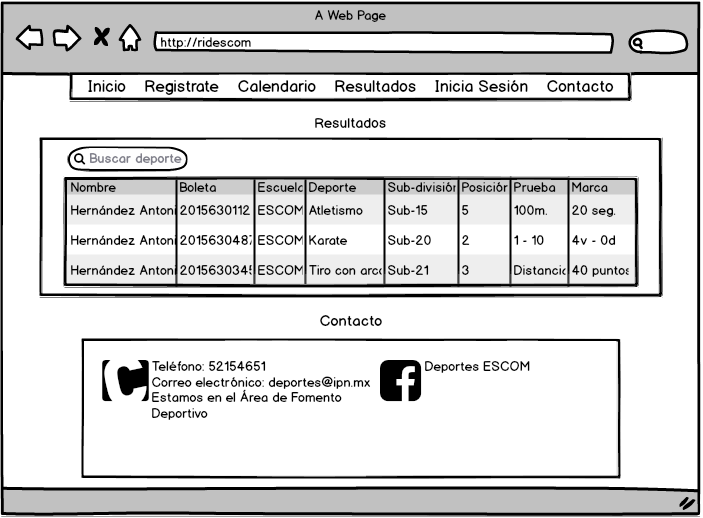
\includegraphics[width=10cm, height=6cm]{Imagenes/Disenos/Iniciogeneral1}
		\caption{Inicio General parte 2}
		\label{inicioGeneral1}
	\end{figure}
	
	\noindent Interfaz Login del Jefe del Departamento de Fomento Deportivo: En esta interfaz ayuda al usuario indicando los elementos que se necesitan para iniciar sesión como usuario de la aplicación (Nombre-Usuario/contraseña previamente registrado), si el usuario no existe el mecanismo realizado en el SPRINT1 se encargará de rechazarlo, podrá recuperar su contraseña en la sección de “¿Olvidaste tu contraseña?”, para mas detalles consulte en el apartado Anexo la Figura 	\ref{inicioJFDycoord}. 
	\newline
	
	\noindent Interfaz Inicio del Jefe del Departamento de Fomento Deportivo: El diseño de la página será muy similar con el resto de los usuarios, sin embargo, este contará con distintas opciones como son: Crear un evento deportivo, Resultados, Calendario y Control de cordinadores donde en este apartado tendrá la opción de Consultar coordinadores, Registrar usuario, Modificar contraseña de los coordinadores de las Unidades Académicas, para mas detalles consulte en el apartado Anexo la Figura 	\ref{principalJFD}. El diseño en general de la vista de este usuario se puede ver en el apartado Anexo \ref{diseños} las Figuras \ref{principalJFD} y \ref{principalJFD1}.
	\newline
	
	\noindent Interfaz Crear un evento interpolitécnico: Dentro de esta vista el Jefe del Departamento de Fomento Deportivo llenaráa los campos para poder dar de alta algún evento, se pedirá el Nombre del evento, Fecha en la que se llevará acabo, Fecha inicio de inscripción y Fecha fin de inscripción, un campo de Descripción donde podrá agregar la dirección del lugar entre otros datos. Se seleccionará el deporte al que corresponde dicho evento, para mas detalles consulte en el apartado Anexo \ref{diseños} la Figura \ref{creaevento}.
	\newline
	
	\noindent Interfaz Registra un coordinador: Se solicitarán datos como Nombre, Apellido Paterno, Apellido Materno,correo electrónico, teleéfonos de contacto y Escuela a la que pertenece, para mas detalles consulte en el apartado Anexo \ref{diseños} la Figura \ref{registrarcoord}.
	
	\noindent Interfaz login coordinador: En esta interfaz ayuda al usuario indicando los elementos que se necesitan para iniciar sesión como usuario de la aplicación (Nombre-Usuario/contraseña previamente registrado), si el usuario no existe el mecanismo realizado en el SPRINT1 se encargará de rechazarlo, para mas detalles consulte en el apartado Anexo \ref{diseños} la Figura \ref{inicioJFDycoord}. En caso de que el coordinador olvide su contraseña deberá ponerse en contacto con el Jefe del Departamento de Fomento Deportivo para solicitar el cambio de contraseña.
	\newline
	
	\noindent Interfaz  Inicio del coordinador de una Unidad Académica: Al igual que el resto de los usuarios en general tiene un diseño muy similar, la diferencia recae en las opciones que puede realizar, en este caso son: Registrar entrenador, Calendario, Resultados, Consulta de inscripciones y Válidar perfil, para mas detalles consulte en el apartado Anexo \ref{diseños} la Figuras 	\ref{principalcoord} y en la Figura \ref{principalcoord1} se puede observar que estará disponible un apartado para publicar algun evento previamente dado de alta en la red social de Facebook.
	\newline
	
	\noindent Interfaz Resultados: Este módulo esta designado para que se ingresen los resultados de los participantes y sean vistos en la página principal. Podrá ingresar hasta 20 datos por vez, para mas detalles consulte en el apartado Anexo \ref{diseños} la Figura \ref{ingresaresultados}.
	\newline
	
	\noindent Interfaz Registro entrenador: En este  módulo el coordinador deberá los campos solicitados tales como: No. Empleado, Nombre, Apellidos, Correo electrónico, Teléfono fijo, Teléfono móvil, asi como definir a que deporte pertenece y por ultimo, especificar si cuenta con un asistente, para mas detalles consulte en el apartado Anexo \ref{diseños} la Figura \ref{registroentrenador}.
	\newline
	
	\noindent Interfaz Login alumno: En esta interfaz ayuda al usuario indicando los elementos que se necesitan para iniciar sesión como usuario de la aplicación (Usuario/contraseña previamente registrado), si el usuario no existe el mecanismo realizado en el SPRINT1 se encargará de rechazarlo, podrá recuperar su contraseña en la sección de “¿Olvidaste tu contraseña?”, para mas detalles consulte en el apartado Anexo \ref{diseños} la Figura \ref{loginalumno}.
	\newline
	
	\noindent Interfaz Inicio del alumno: El diseño de la página será muy similar con el resto de los usuarios, sin embargo, este contará con distintas opciones como son: Inscribir un Interpolitécnico, Calendario, Consulta tus registros y Contacto, como se muestra en el apartado Anexo \ref{diseños}, la Figura 	\ref{principalalum}. El diseño en general de la vista de este usuario, para mas detalles consulte en el apartado Anexo \ref{diseños} la Figuras \ref{principalalum} y \ref{principalalum1}.
	\newline
	
	\noindent Interfaz Inscribir interpolitécnico: En este módulo el alumno primero deberá válidar el estatus de su inscripción, si esta inscrito en el periodo actual, se habilitará el botón para registrar la cédula. En caso contrario el botón no estará habilitado y por tanto, no podrá inscribirse. Los campos que debera llenar el alumno serán: Grupo, NSS (Número de Seguro Social), Lugar de Nacimiento, correo electrónico, Delegación/Municipio, asi como seleccionar el deporte, sub-division y prueba en la que quiere participar, para mas detalles consulte en el apartado Anexo \ref{diseños} las Figuras \ref{Inscripcioninterpolitecnico}.
	\newline
	
	\noindent Interfaz Consulta tus registros: En este módulo, el participante podrá visualizar en una tabla los eventos a los cuales se a registrado, a su vez le mostrará información como: el deporte, prueba Fecha del Evento y la direccion del mismo, para mas detalles consulte en el apartado Anexo \ref{diseños} la Figura \ref{consultainscripcion}.
	\newline
	
	\noindent En este capítulo se presentará una breve descripción del trabajo realizado, los problemas que se enfretaron, así como lo que se logró. Continuando con el capítulo se presentan los Sprint porgramado. 
	De manera breve se hace mención de los casos de uso desarrollados, vistas del proyecto final. así como las pruebas realizadas.
	
	\section{Sprint 4: Módulo de difusión de eventos}
	\noindent Este Sprint se planteó mostrar a los usuarios involucrados en la aplicación web los eventos disponibles al momento, siendo así puedan informarse y decidir los eventos en los que quiera participar. Durante el proceso de desarrollo en Trabajo Terminal 2, se modificó la manera en la que se presentaría estos. 
	En un principio se planteó en mostrar los datos dentro de una tabla como se muestra en la Figura  , sin embargo esto cambió de tal manera que se presentará los datos de cada evento en un recuadro y a su vez estos están ordenados de forma ordenada.
	
	\section{Sprint 5:Módulo de comunicación con redes sociales}	
	\noindent Este Sprint se planteó con la finalidad de hacer llegar por distintos medios, los eventos que están disponibles para su inscripción. De tal manera, se estableció que estos fueran compartidos a través de la red social Facebook.
	Teniendo en cuenta lo antes mencionado, se utiliza la API de Facebook la cual proporciona tanto la documentación, ejemplos y herramientas para que puedan ser ocupadas para su integración en distintos proyectos. \\
	\noindent Lo que se desarrolló fue el iniciar sesión desde la aplicación web “Ridescom”, una vez ingresada a la cuenta se puede realizar la publicación de los distintos eventos desde la misma, viendo reflejado el cambio directamente en el apartado de publicaciones de la página correspondiente en Facebook. \\
	\noindent Para lograr esto como primer paso se creó una cuenta de correo electrónico. Se estableció un correo y contraseña, esto servirá para posteriormente crear una cuenta en la red social de Facebook y a su vez, hacer uso de las herramientas de desarrollo de Facebook.
	A continuación se muestra el momento y datos que se pusieron para crear el correo electrónico.
	
	\begin{figure}[hbt!]
		\centering
		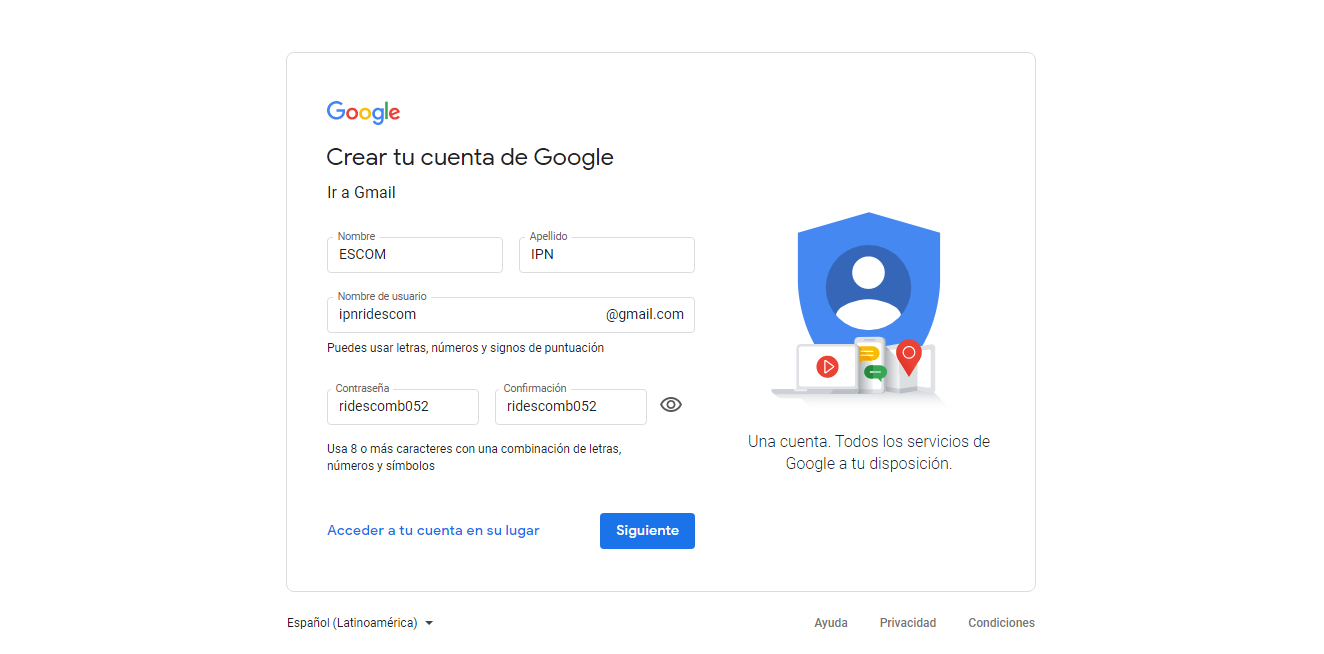
\includegraphics[width=12cm, height=6cm]{Imagenes/CreacionCuentaFB/CuentaGmail}
		\caption{Creacion de la cuenta en Gmail.}
		\label{cuentagmail}
	\end{figure}
	
	
	\noindent Posteriormente se creó la cuenta en la red social facebook, ya que es necesario crear una página en la antes mencionada para la difusión de los eventos. 
	
	\begin{figure}[hbt!]
		\centering
		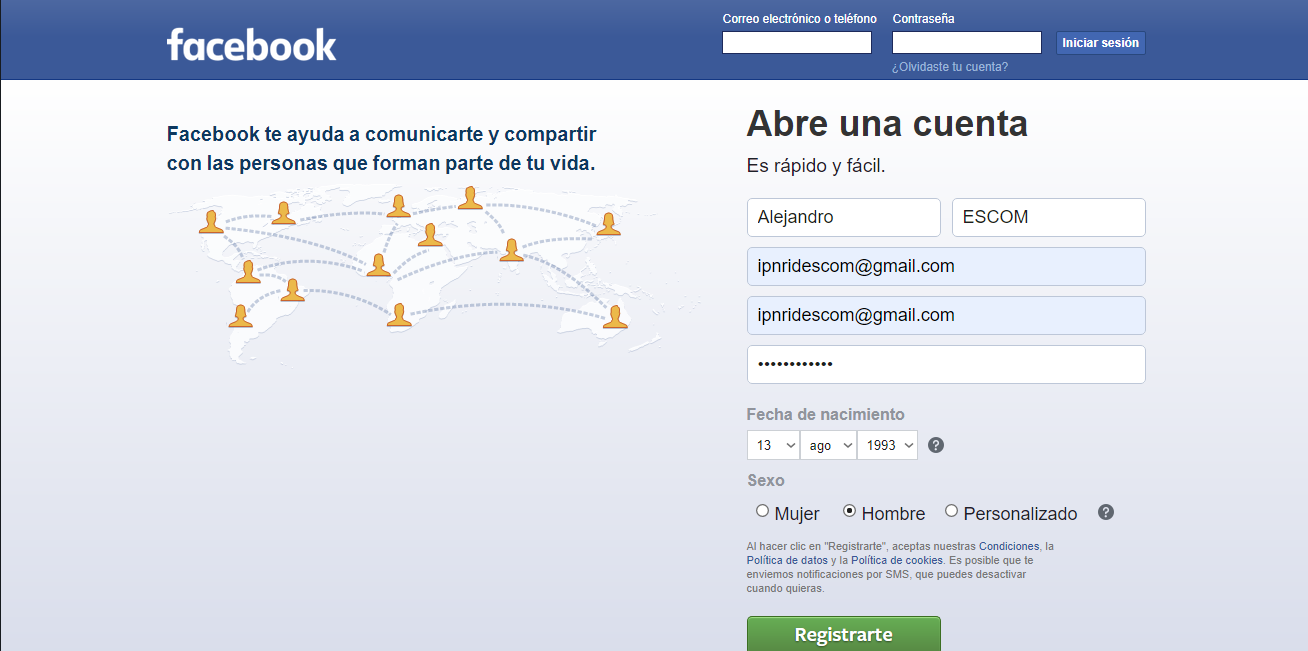
\includegraphics[width=10cm, height=6cm]{Imagenes/CreacionCuentaFB/CreacionCuentaFB}
		\caption{Creación de cuenta en la red social Facebook.}
		\label{creacioncuentafb}
	\end{figure}
	\pagebreak
	
	\noindent Una vez teniendo la cuenta creada se creó la página que se utilizará para la difusión de los eventos. Como se muestra a continuación.
	
	\begin{figure}[hbt!]
		\centering
		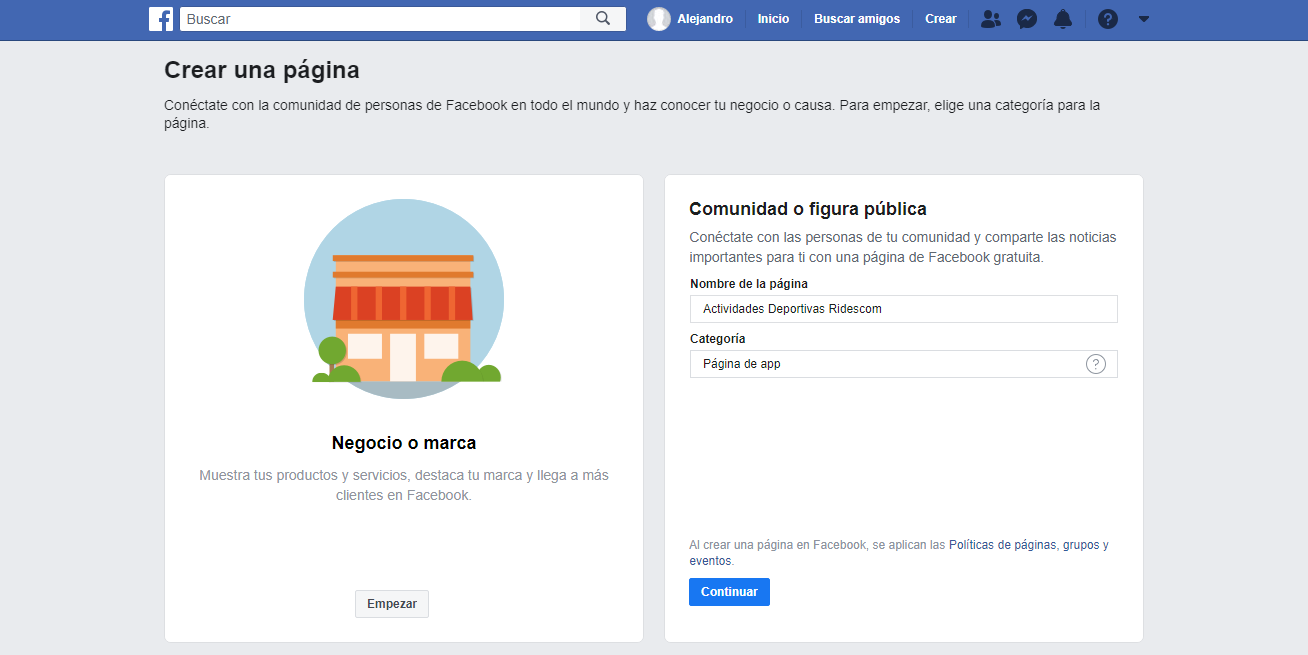
\includegraphics[width=10cm, height=6cm]{Imagenes/CreacionCuentaFB/CreacionPagina}
		\caption{Creación página en Facebook.}
		\label{creacionpagina}
	\end{figure}
	
	
	\noindent Teniendo creada la cuenta y la página en Facebook, desde le herramienta Developers Facebook, se crea una aplicación, la cual tendrá como función el enviar los datos entre nuestra aplicación y la página de Facebook.\\
	
	\noindent Para realizar dicha conexón se accede a la configuración de la aplicación, para que la página que se creó previamente aparezca como una opción para conectar, debe de incluir el nombre de la aplicación (creada en Developers) y en el apartado de categoría se debio seleccionar la opcion de Página de app como se muestra en la Figura \ref{creacionpagina}.
	
	\noindent Al concluir con el proceso de ligar la página de Facebook con la aplicación se muestra el cambio, como se puede apreciar en la Figura \ref{conexionpaginaapp}.
	
	\begin{figure}[hbt!]
		\centering
		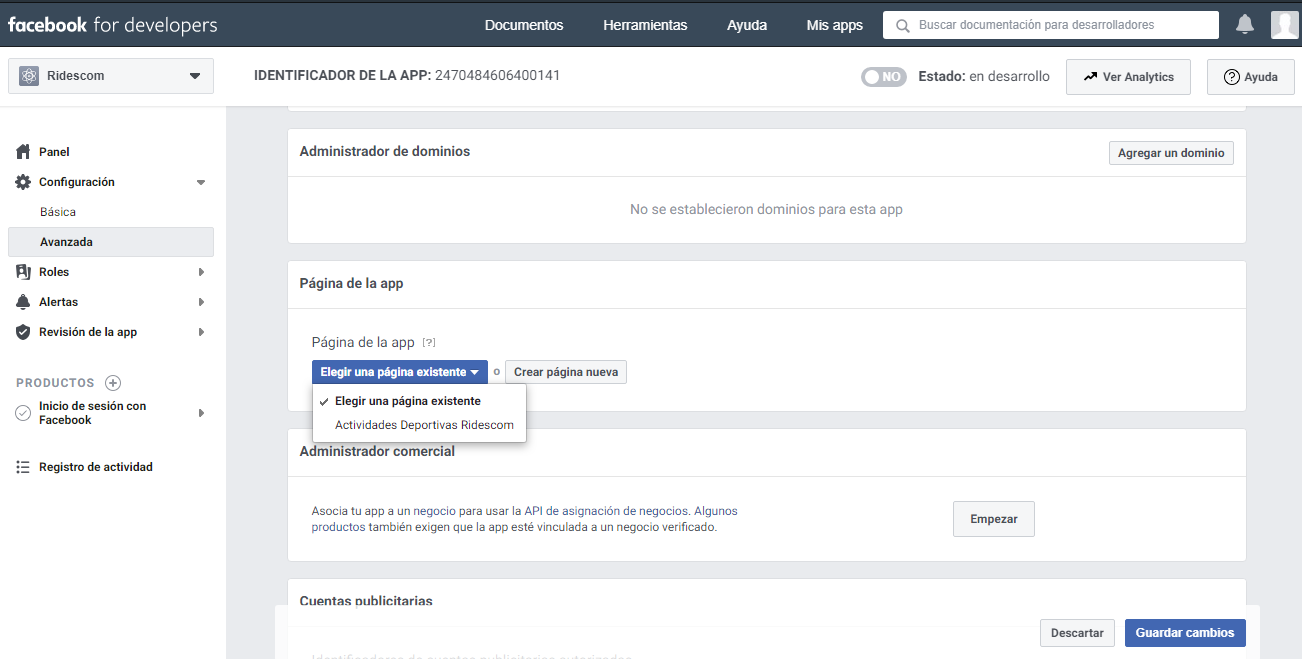
\includegraphics[width=10cm, height=6cm]{Imagenes/CreacionCuentaFB/ConexionPagina}
		\caption{Conexión entre página y aplicación.}
		\label{conexionpaginaapp}
	\end{figure}
	
	
	\noindent Sin embargo, durante el periodo correspondiente a Trabajo Terminal 2 los términos de uso se actualizaron solicitando datos por verificar para poder hacer uso de las herramientas de Facebook. A su vez se cambió la estructura y envío de  datos para una correcta conexión entre las herramientas de Facebook y el proyecto que se está desarrollando, para más detalles consulte el apartado \ref{apiFB}.
	\pagebreak
	
	\section{Sprint 6:Módulo de creación de cédula de inscripción.}
	\noindent Este Sprint se planteó ya que un problema es que se inscribían personas fuera del IPN, con esto se genera automaticamente un listado donde vienen los alumnos inscritos en cada uno de los eventos.
	Para el desarrollo de este módulo se realizó una investigación de un pluggin o herramienta que sea compatible y de fácil implementación para la generación de un reporte. Una vez realizada la investigación se decidió usar la herramienta iReport, la cual tiene facilidad al integrarla al proyecto y facilidad al hacer uso de la misma. Una vez agregado el pluggin que nos permite hacer uso de la misma, se hizo de un análisis de los parámetros que se iban a mostrar en el reporte. Se definió un formato único que será utilizado por las distintas Unidades Académicas, a su vez se definió que será en formato PDF ya que así, se puede apoyar a la mitigación de edición de datos de los participantes. Al descargar el formato, el Coordinador podrá visualizar un listado de los participantes que se inscribieron en algún evento iterpolitécnico deportivo durante las fechas establecidas.
	
	
	\section{Sprint 7: Módulo de consulta de resultados.}
	\noindent Este Sprint se planteó con la finalidad de que los actores involucrados en la aplicación web puedan visualizar los resultados obtenidos por los alumnos participantes en los eventos interpolitécnicos deportivos. 
	Estos se mostrarán en una tabla con los datos más relevantes de estos, cabe destacar que se agrega un módulo para el participante el cual es “Historial”, la finalidad de este es para que el alumno pueda ver de manera fácil y rápida los eventos en los que a participado a lo largo de su trayectoria académica complementando con los datos relacionados a los resultados de los mismos.
	
	%=========================================================
	%                                                         Sprint 0
	%=========================================================
	\section{Sprint 0: Análisis}
	\noindent En este SPRINT se declara el planteamiento y comportamiento de la aplicación como tal, en sus inicios, el plan de desarrollo y los posibles resultados que otorgará.
	Este no se contempló en inicios del proyecto, sin embargo es de importancia ya que en este se definen, las herramientas \ref{Herramientas} que se van a emplear, el análisis del sistema, visualizar y proponer el proceso que se emplea.
	También se especificará cómo es que se instalaron las herramientas empleadas.
	
	\noindent Dentro de este Spring se reunió con responsable de las actividades del Departamento de Formación Deportivas para que se planteara la problematica y así, se defina que es lo que se puede atacar con el proyecto, ver el proceso detalladamente para la inscripción a un evento interpolitécnico deportivo \ref{Entrevista}, se plantearon los Casos de Uso. 
	
	\noindent Cabe destacar que durante el desarrollo correspondiente a Trabajo Terminal 2, nos percatamos de que existia cierta inconsistencia en la relación de algunas tablas a lo cual se realizó la modificación para mas detalles de la estructura actual de la base de datos consulte el apartado Anexos la sección D \ref{CasosdeUso},está se modelo de tal forma que ya contempla el agregar otras unidades académicas\ref{BasedeDatos}. 
	
	\noindent Ahora bien, en este apartado se muestra la estructura propuesta en Trabajo Terminal, como se muestra en la Figura \ref{basededatosInicial}. 
	\pagebreak
	
	\begin{figure}[hbt!]
		\centering
		\includegraphics[angle=90, width=10cm, height=15cm]{Imagenes/BasedeDatos}
		\caption{Base de Datos propuesta en Trabajo Terminal 1.}
		\label{basededatosInicial}
	\end{figure}
	
	\noindent Los cambios realizados fueron respecto a la tabla de Tipo de Contacto, esta se cambio por la separación del tipo de contacto. Quedando tres tablas nuevas, las cuales son: Telefonono Fijo, Telefonono Celular y extensión. \\
	Otro cambio realizado fue la relación entre la tabla Evento y la tabla Act Deportiva, con el cambio realizado quedó la tabla Evento relacionada con la tabla Prueba. Con la finalidad de encontrar especifícamente los datos de un evento en particular, ya que nos percatamos que con la primer relación se mostraban datos duplicados. 
	
	%=========================================================
	%                                                         Sprint 1
	%=========================================================
	\section{Sprint 1:  Mecanismo de validación de estatus académico.}
	\noindent Para el desarrollo de este Sprint se desarrolla la forma de verificar el estatus académico de los alumnos que deseen participar en un evento interpolitécnico. \\
	Dicha verificación consiste de 3 pasos:
	\begin{enumerate}
		\item Ingresa credenciales en la aplicación web RIDESCOM.
		\item Se verifican credenciales en el SAES.
		\item Accede a la página RIDESCOM.
	\end{enumerate}
	
	Como primer paso, el usuario ingresa el usuario y contraseña, mismas que ocupa para ingresar al Sistema de Administración Escolar SAES.
	Una vez ingresado Usuario y Contraseña, la aplicación hace uso del Crawler \ref{crawler}. \\
	Este tomará la información de Usuario y Contraseña, las utilizará para ingresar al SAES, de tal manera que se comprobará si estas son correctas o no. En cualquier caso, se tomará la respuesta para mostrala al usuario.
	Finalmente, en la aplicación web se buscará la respuesta del Crawler para definir el acceso a la aplicación.
	
	El objetivo de este mécanismo es comprobar la inscripción del alumno en el IPN, ya que en el reglamento en el que se basan los eventos interpolitécnicos deportivos, donde se menciona que solo deben participar alumnos que estén inscritos. \ref{crawler}
	
	
	\section{Sprint 3: Módulo de formulario}	
	\noindent En el desarrollo de este Sprint se desarrollaron los formulario necesario para el proyecto, sin embargo, en el proceso de desarrollo se optó por implementar un Crawler, el cual ayudaría a reducir vistas y manejo de información al comprobar los datos de un alumno. Siendo así, los formularios desarrollados son: agregar, editar y eliminar deporte, agregar, editar y eliminar coordinador de unidad académica, agregar, editar y eliminar evento, agregar, editar y eliminar pruebas, inscribir interpolitecnico.
	
	
		
	%=========================================================
	%                                                         Capitulo 6 Desarrollo
	%=========================================================
	%\chapter{Trabajo a futuro}
	En este apartado lo que se describe es lo que se tiene y lo que se entregará
	
	%=========================================================
	%                                                         Capitulo 7 Pruebas
	%=========================================================
	\chapter{Pruebas}

	\noindent En este capítulo se presentará una breve descripción acerca de las distintas pruebas realizadas, los resultados obtenidas en casa una de ellas, así como el procedimiento que se siguio.
	Se mencionarán distintos tipos de pruebas realizadas con la finalidad de omitir lo más posible los errores que puedan presentarse siendo usada por los usuarios finales. \\
	
	\section{Plan de pruebas}
	\noindent La finalidad de realizar pruebas antes de que el proyecto sea entregado al usuario final es mitigar en su mayoría o totalidad los posibles errores que puedan presentarse, de tal manera que, para el equipo de desarrollo se le informa de errores que pudieron omitirse durante el análisis del mismo y a su vez proporciona confianza al cliente en cuanto al funcionamiento del proyecto.
	
	\noindent Por tal motivo se llegó a la conclusión de realizar pruebas al proyecto propuesto para identificar posibles errores que no se contemplaron en el análisis del mismo y lo más importante, proporcionarle al usuario final una aplicación web que no tenga fallos constantes. 
	
	\noindent Las primeras pruebas que se realizaron fueron las pruebas unitarias, las cuales consistieron en realizar pruebas sencillas de tal manera que se comprobara que al hacer uso de cada módulo desarrollado no tuviese errores.\\
	Mencionando algunas de las pruebas fue el verificar que en las entradas de un formulario no presentará errores, se comprobó que existiesen los mensajes y validaciones previamente definidas.
	
	\noindent Posteriormente se realizaron pruebas de sistema, estas consisten en ir agregando de manera progresiva los módulos desarrollados y, que cumpliesen con las pruebas unitarias. De tal manera, se verifica que la conexión entre distintas vistas o módulos tuvieran un buen resultando tomando en cuenta los mensajes y validaciones previamente definidos. \\
	
	\noindent Una vez que se concluyeron las pruebas de sistema nos acercamos con alumnos de la Escuela Superior de Cómputo para informarles en primer instancia, el funcionamiento del proyecto, a quién va dirigido y algunos puntos relevantes del desarrollo del mismo con lo antes mencionado se obtuvo lo siguiente:
	
	\begin{figure}[hbt!]
		\centering
		\includegraphics[width=8cm, height=8cm]{Imagenes/tablaEstadisticas}
		\caption{Tabla del número de alumnos considerados para las pruebas.}
		\label{tablaestadisticas}
	\end{figure}

	\begin{figure}[hbt!]
		\centering
		\includegraphics[width=8cm, height=6cm]{Imagenes/graficaEstadisticas}
		\caption{Gráfica corresponidente a la Tabla de alumnos considerados para las pruebas.}
		\label{graficaestadisticas}
	\end{figure}
	
	\noindent Considerando los resultados obtenidos, se recabó información de errores que no se habían contemplado. Otro punto importante fue el porcentaje de alumons que se negaron a participar en la prueba del proyecto sin embargo, con los datos obtenido se logró obtener una mejora en el proyecto. 
	
	\noindent No obstante, para complementar la etapa de pruebas del proyecto nos basamos en las pruebas Clases de Equivalencia. En la cual se se plantean los posibles casos que se pueden llegar a presentar en un módulo. Estos casos se crean o toman con base en el caso de uso correspondiente, es decir, por cada caso de uso que se tiene en el sistema debe existir un guión de prueba.\\
	
	\noindent La ventaja con este tipo de pruebas es que nos permite cubrir todos los posibles escenarios en un módulo en específico. Para saber el número de pruebas que son necesarias realizar se debe seguir la siguiente formula matemática:\\
	$ n1 * n2 * ... * n_{n} $ \\
	donde, 
	n, corresponde al número de entradas que tiene el caso de uso.\\
	n1, este valor corresponde al número de pruebas que se realicen en cada uno de las entradas del caso de uso.\\
	
	\noindent Ahora bien, hay otra formula la cual indica el número de pruebas minímas necesarías para considerar que el caso de uso analizando tiene cálidad, la formula matemática es la siguiente: \\
	
	$ (n1 + n2 + ... + n_{n}) - (n - 1) $
	
	n, corresponde al número de entradas que tiene el caso de uso.\\
	n1, este valor corresponde al número de pruebas que se realicen en cada uno de las entradas del caso de uso.\\
	
	\noindent Tomando en cuenta lo antes mencionado, se realizaron las pruebas correspondientes, a continuación se mostrarán los guiónes de prueba de alguno de los módulos representativos de la aplicación web.\\
	\pagebreak
	
	\textbf{Guión de prueba del caso de uso 10: Agrega resultados}
	
	\begin{figure}[hbt!]
		\centering
		\includegraphics[width=14cm, height=6cm]{Imagenes/Pruebas/GuionPruebaCU10}
		\caption{Tabla correspondiente al guión de prueba del caso de uso 10}
		\label{guionpruebaCU10}
	\end{figure}

	\textbf{Guión de prueba del caso de uso 11: Agrega resultados}

	\begin{figure}[hbt!]
		\centering
		\includegraphics[width=14cm, height=6cm]{Imagenes/Pruebas/GuionPruebaCU11}
		\caption{Tabla correspondiente al guión correspondiente al CU11}
		\label{guionpruebaCU11}
	\end{figure}
\pagebreak

	\textbf{Guión de prueba del caso de uso 11: Agrega resultados}
	\begin{figure}[hbt!]
		\centering
		\includegraphics[width=14cm, height=6cm]{Imagenes/Pruebas/GuionPruebaCU11_1}
		\caption{Tabla correspondiente al guión correspondiente al CU11}
		\label{guionpruebaCU11_1}
	\end{figure}

	\textbf{Guión de prueba del caso de uso 15: Agrega resultados}
	\begin{figure}[hbt!]
		\centering
		\includegraphics[width=14cm, height=6cm]{Imagenes/Pruebas/GuionPruebaCU15}
		\caption{Tabla correspondiente al guión correspondiente al CU15}
		\label{guionpruebaCU15}
	\end{figure}
\pagebreak
	
	\textbf{Guión de prueba del caso de uso 16: Agrega resultados}	
	\begin{figure}[hbt!]
		\centering
		\includegraphics[width=14cm, height=6cm]{Imagenes/Pruebas/GuionPruebaCU16}
		\caption{Tabla correspondiente al guión correspondiente al CU16}
		\label{guionpruebaCU16}
	\end{figure}
	
	\textbf{Guión de prueba del caso de uso 22: Agrega resultados}	
	\begin{figure}[hbt!]
		\centering
		\includegraphics[width=14cm, height=6cm]{Imagenes/Pruebas/GuionPruebaCU22}
		\caption{Tabla correspondiente al guión correspondiente al CU22}
		\label{guionpruebaCU22}
	\end{figure}
	
	
	
	
	%=========================================================
	%                                                         Capitulo 7 Pruebas
	%=========================================================
	\chapter*{Conclusiones}
\phantomsection
\addcontentsline{toc}{chapter}{Conclusiones}
	\noindent 
	En este capítulo se presentará una breve descripción acerca del trabajo terminal haciendo mención del trabajo que se realizó, los problemas que se enfrentaron, así como lo que se logró. Continuando con el capítulo se presentan las Reglas de Negocio y las Reglas del Sistema donde se menciona que es lo que puede realizar la aplicación y que no.\\
	
	
	%=========================================================
	%                                                         Capitulo 7 Pruebas
	%=========================================================
	\chapter*{Trabajo a Futuro}
\phantomsection
\addcontentsline{toc}{chapter}{Trabajo a Futuro}
	En este capítulo se presentará una breve descripción acerca del trabajo terminal haciendo mención del trabajo que se realizó, los problemas que se enfrentaron, así como lo que se logró. Continuando con el capítulo se presentan las Reglas de Negocio y las Reglas del Sistema donde se menciona que es lo que puede realizar la aplicación y que no.\\
	

	%=========================================================
	%     										Referencias
	%=========================================================
	
\begin{thebibliography}{}

	\bibitem{hist} 
		\textit{S. Luján Mora}
		\textsc{Programación de aplicaciones web: historia, principios básicos y clientes web} [En línea].
		 

		Disponible en 
		\url{https://gplsi.dlsi.ua.es/~slujan/materiales/pi-cliente2-muestra.pdf}

	\bibitem{mor} 
		\textit{M. Peréz.}
		\textsc{Atletismo y Tiro con Arco en Morelos.} [En línea].
		 

		Disponible en 
		\url{https://www.lajornadamorelos.com.mx/deportes/2019/01/31/7673}
%==== Reglamento interpolitecnicos deportivos===%
	\bibitem{Reglas} 
		\textsc{E. A. Venegas López.}
		\textit{Convoca a las unidades académicas del I.P.N. a participar en la liga interpolitecnica 2018 "Juan de Dios Bátiz Paredes".} [En línea]. Instituto Politécnico Nacional Secretaría de Servicios Educativos, México, 2018.
		 

		Disponible en
		\url{http://deportes.ipn.mx/docs/inter2018/general.pdf}


	\bibitem{spring} 
		\textit{Depto. Ciencia de la computación e IA.}
		\textsc{Spring.} [En línea]. 
	    

		Disponible en:
		\url{http://www.jtech.ua.es/j2ee/publico/spring-2012-13/wholesite.pdf}

	\bibitem{MVC} 
		\textit{M. A. Sánchez Rico.}
		\textsc{Capítulo 3: Spring, un framework de aplicación.} [En línea].
		 

		Disponible en:
		\url{http://catarina.udlap.mx/u_dl_a/tales/documentos/lis/sanchez_r_ma/capitulo3.pdf}

	\bibitem{BD} 
		\textit{E. García Cano.}
		\textsc{Notaciones de modelado de bases de datos.} [En línea]. México.
		 

		Disponible en:
		\url{https://www.academia.edu/20435604/Notaciones_de_modelado_de_bases_de_datos?fbclid=IwAR0jlb2ddOVgIQByreQg9H-84RuMrG_JQeR0Z4E61-R_E08eejb97PuPEmM}

	\bibitem{BD1}
		\textit{Á. M. del Pilar \& Arellano Mendoza L. P.}
		\textsc{Manual de prácticasdel Laboratorio de Bases de Datos.} [En línea]. México. pp. 16-17
		 

		Disponible en: 
		\url{http://odin.fi-b.unam.mx/salaD/practicasBD/manualBD.pdf?fbclid=IwAR1iluFg_wBYfHof_6B5T3jhHZqhGZ2BOEXhiYJ07IRUsY5fxt-r0JOUXOs}	

	
	\bibitem{book} 
		\textit{T. Satpathy}
		\textsc{Una guía para el CUERPO DE CONOCIMIENTO DE SCRUM (GUÍA SBOK^{TM}).} [En linea]. pp. 51-63 
		

        \url{https://www.tenstep.ec/portal/images/pdfs/Suscripciones_TenStep/Silver/SCRUMstudy_GUIA_SBOK_espanol.pdf}
        
    %=== Referencias protocolo
	\bibitem{Reglamento}
			\textsc{I.P.N.}
			\textit{Secretaría de Servicios Educativos Dirección de Desarrollo y Fomento Deportivo General Liga Interpolitécnica.}
	  [En línea]. México, 2018.
		

		Disponible en: 
		\url{http://deportes.ipn.mx/docs/inter2018/Rparticipacion.pdf}

	\bibitem{Entrevista}
			\textsc{A. Miranda de Olmo.} 
	        \textit{Entrevista con el jefe de actividades culturales y deportivas de la ESCOM.} México, 2019.
	

	\bibitem{problema}
		\textit{B. Jones.}
		\textsc{4 problemas en el deporte juvenil de hoy.} [En línea].
		 VANGUARDIA. México 2015.
		
		Disponible en: 
		\url{https://vanguardia.com.mx/4problemaseneldeportejuvenildehoy-2310350.html}

   \bibitem{problemas}
		\textit{E. Macedo de Mereidos.}
		\textsc{Problemas del deporte son globales y las soluciones han de serlo.} [En línea]. 
		MundoDeportivo. España. 2016.
		
		Disponible en: 
		\url{https://www.mundodeportivo.com/otros-deportes/20161007/41845726098/problemas-del-deporte-son-globales-y-las-soluciones-han-de-serlo-dice-icss.html}
		
	\bibitem{guia}
		\textit{J. Palacios.}
		\textsc{Guía fundamental de SCRUM.} [En línea]. 
         Jerónimo Palacios \& associates. 
		
		Disponible en: 
		\url{https://jeronimopalacios.com/scrum/}
		
	\bibitem{scrum}
		\textit{L. N. Medina Velandia \& W. M. López López.}
		\textsc{ESCOGER UNA METODOLOGÍA PARA DESARROLLAR SOFTWARE, DIFÍCIL DECISIÓN.} [En línea]. 
		  Revista Educación en Ingeniería ISSN 1900-8260. pp.102. 2015. 
		
		Disponible en: 
		\url{https://www.educacioneningenieria.org/index.php/edi/article/viewFile/579/275}
		
		%==== Aplicaciones 
	\bibitem{TUni}
		\textsc{TU University.}
		%\textit{} 
		[En línea]. 
		
		Disponible en: 
		\url{https://support.teamunify.com/en/articles/450}
		
	\bibitem{IND} 
		\textit{Instituto Nacional de Deportes.}
		\textsc{}[En línea].
		

		Disponible en:
		\url{http://www.proyectosdeportivos.cl/SPP/index.aspx}
	
	\bibitem{cono} 
		\textsc{}
		\textit{Concurso Once.} [En línea].
		
		Disponible en:
		\url{https://www.concursoescolaronce.es/unete-participa/}

	\bibitem{team} 
		\textit{}
		\textsc{TeamSnap Tournament.} [En línea].
		

		Disponible en:
		\url{https://www.teamsnap.com/tournaments}
		
	\bibitem{po} 
		\textsc{}
		\textit{PlayyOn.} [En línea].
		

		Disponible en:
		\url{https://www.playyon.com/login/?next=/admin/}
		
	\bibitem{tp}
		\textit{}
		\textsc{TorneoPal.} [En línea].
		
		
		Disponible en: 
		\url{ https://www.torneopal.com/tournament-management-software/}
		
	\bibitem{act}
		\textit{}
		\textsc{Active Network.} [En línea].
		 
		
		Disponible en: 
		\url{http://www.activesports.com/sports-solutions/by-feature/sports-league-management}
		
	\bibitem{ts}
		\textit{}
		\textsc{Tournament Software.} [En línea].
		 
		
		Disponible en: 
		\url{https://www.tournamentsoftware.com/Home}
	
	\bibitem{gpi}
		\textit{M. Trigas Gallego.}
		\textsc{Gestión de Proyectos Informaticos. Metodologpia SCRUM.} [En línea].

		
		Disponible en: 
		\url{http://openaccess.uoc.edu/webapps/o2/bitstream/10609/17885/1/mtrigasTFC0612memoria.pdf}	
		
	\bibitem{mex}
		\textit{D. Mancera, A. Dabdoub \& E. Camhaji.}
		\textsc{¿Que le pasa al deporte en México?} [En línea].
		 EL PAÍS. México. 2016.

		
		Disponible en: 
		\url{https://elpais.com/deportes/2016/08/27/actualidad/1472309744_847142.html}	

    \bibitem{mu}
		\textit{P. Vallejo.}
		\textsc{El deporte y la crisis mundial. Propuesta curricular para la Educación Física Secundaria.} [En línea]. 
	    efdeportes.com. Argentina. 2009.
		
		Disponible en: 
		\url{http://www.efdeportes.com/efd131/el-deporte-y-la-crisis-mundial.htm}

\end{thebibliography}
	
	
	%=========================================================
	%             apendice              Glosario
	%=========================================================
		\chapter*{Glosario}
\phantomsection
	Para el mejor entendimiento de este documento se enlistaron las diferentes palabras y términos que a lo largo del documento y en la propia aplicación se utilizan, y una descripción de los mismos, con el objetivo de contextualizar al lector y comprender mejor la aplicación, su estructura, lo que esta realiza y la interacción que tiene con el usuario final.
	\begin{itemize}
		\item \textbf{Actividad deportiva:} Tiempos, espacios y equipos deportivos ofrecidos por parte de la ESCOM hacia los alumnos para complementar su formación.
		\item \textbf{Alumno:} Persona que cuenta con un número de boleta y está inscrito en la ESCOM. Además debe estar registrado en el sistema. 
		\item \textbf{Aplicación Web:} Aplicación que los usuarios pueden utilizar accediendo a un servidor web a través de Internet o de una intranet mediante un navegador.
		\item \textbf{Área:}
		\item \textbf{Base de datos:} Conjunto de datos pertenecientes a un mismo contexto y almacenados sistemáticamente para su posterior uso. 
		\item \textbf{Boleta:} Identificador único de cada alumno dentro del IPN, a usar dentro del sistema, proporcionado por el IPN a los alumnos inscritos. 
		\item \textbf{Cédula de inscripción:} Documento identificativo utilizado para la inscripción de personas para eventos deportivos.
		\item \textbf{Contraseña:} Clave de acceso conformada por caracteres alfanuméricos asociada a una boleta o número de empleado.
		\item \textbf{Entorno de desarrollo integrado / IDE:} Aplicación informática que proporciona servicios integrales para facilitarle al desarrollador o programador el desarrollo de software. 
		\item \textbf{Escuela Superior de Cómputo / ESCOM:}  Institución pública mexicana de educación superior perteneciente al Instituto Politécnico Nacional. 
		\item \textbf{Iniciar sesión:} Sección del sistema que autentica al usuario mediante una boleta o un número de empleado y una contraseña, permitiéndonos identificar su tipo (alumno, profesor) brindándole acceso a su perfil. 
		\item \textbf{Instituto Politécnico Nacional:} Institución pública mexicana de investigación y educación en niveles medio superior, superior y posgrado. 
		\item \textbf{Interpolitécnico:} Evento competitivo que es desarrollado en el Instituto Politécnico Nacional (IPN) con la finalidad de fortalecer el sistema de competición integral de los alumnos en alguna disciplinas.
		\item \textbf{Número de empleado:} Identificador único de cada profesor dentro del IPN, a usar dentro del sistema, proporcionado por el IPN a los profesores contratados. 
		\item \textbf{Requisito funcional:} Función del sistema de software o sus componentes. Función es descrita como un conjunto de entradas, comportamientos y salidas. 
		\item \textbf{Requisito no funcional:} Requisito que sabe bien y especifica criterios que pueden usarse para juzgar la operación de un sistema en lugar de sus comportamientos específicos, ya que estos corresponden a los requisitos funcionales. 
		\item \textbf{Requisito de Negocio:} Estas definen los límitantes de la aplicación, a su vez delimitan procesos involucrados en la aplicación. También se especifíca como usar correctamente los distintos módulos de la aplicación.
		\item \textbf{Servicio Web:} Tecnología que utiliza un conjunto de protocolos y estándares que sirven para intercambiar datos entre aplicaciones.
		\item \textbf{Servidor:} Aplicación software en ejecución capaz de atender las peticiones de un cliente y devolverle una respuesta en concordancia.
		\item \textbf{Sistema gestor de base de datos / SGBD:} Conjunto de programas que permiten el almacenamiento, modificación y extracción de la información en una base de datos, además de proporcionar herramientas para a~nadir, borrar, modificar y analizar los datos.
		\item \textbf{Software:} Conjunto de programas y rutinas que permiten a la computadora realizar determinadas tareas.
		\item \textbf{Unidad de aprendizaje:} Curso impartido en la ESCOM y que tiene la intención educativa para que se apliquen y se adquieran conocimientos con el n de que los alumnos desarrollen competencias como el pensamiento estratégico, el pensamiento creativo, trabajo colaborativo, trabajo participativo, ética, manejo de conflictos, responsabilidad social, comunicación asertiva, actitud emprendedora.
		\item \textbf{Usuario:} Conjunto de permisos y de recursos (o dispositivos) a los cuales se tiene acceso. Es decir, un usuario puede ser tanto una persona como una máquina, un programa, etc.
	\end{itemize}


	
	%=========================================================
	%                                                         Anexos
	%=========================================================
		\appendix
\clearpage
\addappheadtotoc
\appendixpage
	
	\chapter{Apartado A: Entrevista}
	\label{Entrevista}
	\noindent Entrevista con responsable de las actividades del Departamento de Formación Deportiva
	Buenas tardes, agradecemos el tiempo que nos esta brindando para mostrarle nuestra propuesta de Trabajo Terminal con la cual se pretende ayudar en el proceso de inscripción para los alumnos.
	
	\begin{enumerate}
		\item ¿Cuál es el proceso actual para la inscripción a un evento interpolitécnico?\\
		El alumno tiene que acudir al departamento de Actividades Deportivas de su unidad académica, informar que quiere participar en un evento inrtepolitécnico. Con esto el coordinador procede a solicitar una identificación o documento probatorio que compruebe el estatus académico del alumno, a la vez el coordinador le proporciona una cédula de inscripción para que sea llenada y entrada. Si esto cumple puede continuar con su proceso en caso contrario se detiene el trámite. En cualquiera de los dos caso el alumno es informado del resultado final.
		
		\item ¿Hay límite de edad para los participantes?
		Claro, tomando en cuenta el reglamento esta estipulado que la edad miníma de los participantes es de 18 años y la máxima es de 27 años.
		
		\item ¿Se tiene un formato definido para la inscripción?
		Actualmente no contamos con un formato en especifíco, sin embargo se trata de seguir un formato. Desafortunadamente no todos los Coordinadores de las Unidades Académicas no lo siguen de la manera correcta.\\ 
		Para nosotros esto representa mucho más tiempo para emplear al unificar el formato de la información y tratar de mitigar un poco la dificultad al buscar datos de los participantes.
		
		\item ¿Es necesario la comprobación de inscripción de los alumnos?
		Por supuesto, de igual manera tomando en cuenta el reglamento se especifíca que los alumnos solo podrán participar en un evento siempre y cuando este esté inscrito en el periodo actual al del evento de su interés.\\
		Desafortunadamente, nos hemos percatado de que se han inscrito alumnos que no cumplen con este requisito.
		
		\item ¿Cuántos deportes hay actualmente practicándose en el IPN?
		Actualmente en el Instituto Politécnico Nacional se practican 27 deportes.
		
		\item ¿Se cuenta con algún método de verificación de datos?
		No, es por esta razón que nos hemos percatado hasta el momento de hacer la publicación de resultados que se inscriben alumnos que no están inscritos o personas ajenas al mismo.
		
		\item Una vez concluido los eventos, ¿Qué sigue?
		Se realiza el pago del arbitraje de los eventos, hasta que se haga dicho pago nos es proporcionado los resultados de los participantes.\\
		Teniendo estos, procedemos a realizar el vaciado de los datos para posteriormente sea publicado y así, los participantes puedan ver su desempeño.
		
		\item ¿Cuánto tiempo suele tardarse en la publicación de los resultados?
		En el mejor de los casos nos toma al rededor de una semana, muchas veces esto depende del pago del arbitraje. En algunas ocasiones nos hemos tomado hasta un mes o mes y medio en la publicación de los resultados. 
		
		\item ¿Qué puntos se consideran en la generación de estadísticas?
		Se toman en cuenta la participación de los alumnos por escuela, posteriormente se límita a la cantidad de hombres y mujeres que participaron. También se toma en cuenta la participación por el deporte tomando en cuenta los parametros antes mencionados.
		
	\end{enumerate} 
	
	\chapter{Apartado B: Mensajes}
	\noindent En este apartado, se describen a detalle los mensajes que se encuentran dentro de la aplicación web. Estos mensajes contemplan la notificación de un proceso completado o un error en algún proceso del mismo.
		\section{Mensajes de RIDESCOM}

%===========================  MSG1 ==================================

\begin{mensaje}{MSG1}{Faltan campos por completar}{Error}

	\item[Canal:] Sistema.

    \item[Propósito:] Informar al actor que no se puede realizar el Inicio de sesión ya que no ha completado los campos requeridos.

    \item[Redacción:] Debe ingresar los datos del campo Usuario y Contraseña.

    \item[Parámetros:] Ninguno.

    \item[Ejemplo:] Usuario: Usuario, Contraseña: Contraseña.

	%\item[Referenciado por: ] \refIdElem{DIC-UA-COSIE-CU1.3}, \refIdElem{DIC-UA-COSIE-CU1.3.1},  \refIdElem{DIC-UA-COSIE-CU1.3.2}%\refIdElem{DIC-A-CU1}, \refIdElem{DIC-A-CU2}, \refIdElem{DIC-A-CU3}  \refIdElem{DIC-CGC-DPF-CU1.3}

\end{mensaje}
\newline


%===========================  MSG32 ==================================

\begin{mensaje}{MSG2}{Los datos ingresados no son correctos}{Error}
	
	\item[Canal:] Sistema.
	
	\item[Propósito:] Informar al actor que no se puede realizar el Inicio de sesión ya que los datos ingresados no coinciden con los almacenados.
	
	\item[Redacción:] Debe ingresar los datos correctos del campo Usuario y/o Contraseña.
	
	\item[Parámetros:] Ninguno.
	
	\item[Ejemplo:] Usuario: Usuario, Contraseña: Contraseña.
	
	%\item[Referenciado por: ] \refIdElem{DIC-UA-COSIE-CU1.3}, \refIdElem{DIC-UA-COSIE-CU1.3.1},  \refIdElem{DIC-UA-COSIE-CU1.3.2}%\refIdElem{DIC-A-CU1}, \refIdElem{DIC-A-CU2}, \refIdElem{DIC-A-CU3}  \refIdElem{DIC-CGC-DPF-CU1.3}
	
\end{mensaje}
	
		\pagebreak
		
	\chapter{Apartado C: Diseños de Pantallas}
	\label{diseños}
	\noindent Este apartado, se muestran los diseños de pantallas que se consideraron para incluir en el proyecto final. Se muestran los distintos módulos de cada uno de los participantes involucrados en la aplicación web.
	
		\begin{figure}[hbt!]
			\centering
			\includegraphics[width=10cm, height=6cm]{Imagenes/Nuevos/P1_LoginJFD_coord}
			\caption{Inicio sesión para el JFD y el coordinador de U.A.}
			\label{inicioJFDycoord}
		\end{figure}
		\pagebreak
		
		\begin{figure}[hbt!]
			\centering
			\includegraphics[width=10cm, height=6cm]{Imagenes/Nuevos/P2_Inicio_JefeFD}
			\caption{Página principal para el Jefe de Fomento Deportivo}
			\label{principalJFD}
		\end{figure}
	
		\begin{figure} [hbt!]
			\centering
			\includegraphics[width=10cm, height=6cm]{Imagenes/Nuevos/P3_Inicio_JefeFD1}
			\caption{Página principal para el Jefe de Fomento (Continuación).}
			\label{principalJFD1}
		\end{figure}
	
		\begin{figure} [hbt!]
			\centering
			\includegraphics[width=10cm, height=6cm]{Imagenes/Nuevos/P25_Pruebas_JFD}
			\caption{Página para visualizar las pruebas dadas de alta. (Jefe de Fomento Deportivo)}
			\label{pruebas}
		\end{figure}
		\pagebreak
		
		\begin{figure} [hbt!]
			\centering
			\includegraphics[width=10cm, height=6cm]{Imagenes/Nuevos/P26_AgregarPruebas_JFD}
			\caption{Página para agregar las distintas pruebas pruebas. (Jefe de Fomento Deportivo)}
			\label{agregarpruebas}
		\end{figure}
		
		\begin{figure} [hbt!]
			\centering
			\includegraphics[width=10cm, height=6cm]{Imagenes/Nuevos/P26_EditarPruebas_JFD}
			\caption{Página para editar los datos de las pruebas previamente registrados. (Jefe de Fomento Deportivo)}
			\label{editarpruebas}
		\end{figure}
	
		\begin{figure} [hbt!]
			\centering
			\includegraphics[width=10cm, height=6cm]{Imagenes/Nuevos/P4_Crear_evento_deportivo}
			\caption{Vista para dar de alta un evento deportivo (Jefe de Fomento Deportivo).}
			\label{creaevento}
		\end{figure}
		\pagebreak	
		
		\begin{figure} [hbt!]
			\centering
			\includegraphics[width=10cm, height=6cm]{Imagenes/Nuevos/P27_Deportes_JFD}
			\caption{Página para visualizar los deportes que se llevaran a cabo en los eventos interpolitécnicos}
			\label{deportes}
		\end{figure}
	
		\begin{figure} [hbt!]
			\centering
			\includegraphics[width=10cm, height=6cm]{Imagenes/Nuevos/P28_AgregarDeportes_JFD}
			\caption{Página para agregar un deporte.}
			\label{agregadeporte}
		\end{figure}
		
		\begin{figure} [hbt!]
			\centering
			\includegraphics[width=10cm, height=6cm]{Imagenes/Nuevos/P29_EditarDeportes_JFD}
			\caption{Página para editar datos de los deportes}
			\label{editardeporte}
		\end{figure}
		\pagebreak
		
		\begin{figure} [hbt!]
			\centering
			\includegraphics[width=10cm, height=6cm]{Imagenes/Nuevos/P5_Editar_evento_deportivo}
			\caption{Vista para editar datos de un evento ya registrado. (Jefe de FOmento Deportivo).}
			\label{editarevento}
		\end{figure}
	
		\begin{figure} [hbt!]
			\centering
			\includegraphics[width=10cm, height=6cm]{Imagenes/Nuevos/P6_Registro_coordinador}
			\caption{Vista para registrar un coordinador de unidad académica. (Jefe de Fomento Deportivo).}
			\label{registrarcoord}
		\end{figure}
		
		\begin{figure} [hbt!]
			\centering
			\includegraphics[width=10cm, height=6cm]{Imagenes/Nuevos/P7_Editar_coordinador}
			\caption{Vista para editar datos de un coordinador previamente registrado. (Jefe de Fomento Deportivo).}
			\label{editarcoord}
		\end{figure}
\pagebreak

		\begin{figure} [hbt!]
			\centering
			\includegraphics[width=10cm, height=6cm]{Imagenes/Nuevos/P8_Inicio_CoordUA}
			\caption{Vista principal para el coordinador de una Unidad Académica.}
			\label{principalcoord}
		\end{figure}
	
		\begin{figure} [hbt!]
			\centering
			\includegraphics[width=10cm, height=6cm]{Imagenes/Nuevos/P9_Inicio_CoordUA1}
			\caption{Vista principal para el coordinador de una Unidad Académica (Continuación).}
			\label{principalcoord1}
		\end{figure}
	\pagebreak
		
		\begin{figure} [hbt!] 
			\centering
			\includegraphics[width=10cm, height=7cm]{Imagenes/Nuevos/P10_Ingresa_resultados}
			\caption{Vista para ingresar los resultados obtenidos por los participantes (Coordinador de Unidad Académica).}
			\label{ingresaresultados}
		\end{figure}
		
		\begin{figure} [hbt!]
			\centering
			\includegraphics[width=10cm, height=7cm]{Imagenes/Nuevos/P11_Editar_resultados}
			\caption{Vista para editar los resultados de los participantes (Coordinador de Unidad Académica).}
			\label{editaresultados}
		\end{figure}
		\pagebreak
		
		\begin{figure} [hbt!]
			\centering
			\includegraphics[width=10cm, height=6cm]{Imagenes/Nuevos/P12_Registro_entrenador}
			\caption{Vista para registrar a un entrenador (Coordinador de Unidad Académica).}
			\label{registroentrenador}
		\end{figure}
		
		\begin{figure} [hbt!]
			\centering
			\includegraphics[width=10cm, height=6cm]{Imagenes/Nuevos/P13_Editar_entrenador}
			\caption{Vista para editar los datos del entrenador (Coordinador de Unidad Académica).}
			\label{editarentrenador}
		\end{figure}
		
		\begin{figure} [hbt!]
			\centering
			\includegraphics[width=10cm, height=6cm]{Imagenes/Nuevos/P14_Difundir_evento}
			\caption{Vista para difundir un evento interpolitécnico deportivo (Coordinador de Unidad Académica).}
			\label{difundirevento}
		\end{figure}
		\pagebreak

		\begin{figure} [hbt!]
			\centering
			\includegraphics[width=10cm, height=6cm]{Imagenes/Nuevos/P15_Consulta_alumnos_inscritos}
			\caption{Vista para consultar los alumnos que se han inscrito a un evento (Coordinador de Unidad Académica).}
			\label{consultaalumnosinscritos}
		\end{figure}
	
		\begin{figure} [hbt!]
			\centering
			\includegraphics[width=10cm, height=6cm]{Imagenes/Nuevos/P16_Consulta_para_expedir_constancias}
			\caption{Vista para consultar participación de alumnos (Coordinador).}
			\label{consultaparaexpedirconstancias}
		\end{figure}
		
		\begin{figure} [hbt!]
			\centering
			\includegraphics[width=10cm, height=6cm]{Imagenes/Nuevos/P17_Login_alumno}
			\caption{Vista Inicio de Sesión para el alumno.}
			\label{loginalumno}
		\end{figure}
	\pagebreak
		
		\begin{figure} [hbt!]
			\centering
			\includegraphics[width=10cm, height=6cm]{Imagenes/Nuevos/P18_Inicio_paticipante}
			\caption{Vista principal del alumno.}
			\label{principalalum}
		\end{figure}
		
		\begin{figure} [hbt!]
			\centering
			\includegraphics[width=10cm, height=6cm]{Imagenes/Nuevos/P19_Inicio_paticipante1}
			\caption{Vista principal del alumno (Continuación).}
			\label{principalalum1}
		\end{figure}
	
		\begin{figure} [hbt!]
			\centering
			\includegraphics[width=10cm, height=6cm]{Imagenes/Nuevos/P20_Consulta_Inscripciones}
			\caption{Vista para consultar los eventos a los que se a registrado el alumno (Alumno).}
			\label{consultainscripcion}
		\end{figure}
	\pagebreak
		
		\begin{figure} [hbt!]
			\centering
			\includegraphics[width=10cm, height=6cm]{Imagenes/Disenos/Inscripcioninter}
			\caption{Formulario para que el alumno se registre en un evento interpolitécnico deportivo.}
			\label{Inscripcioninterpolitecnico}
		\end{figure}
		

		\begin{figure} [hbt!]
			\centering
			\includegraphics[width=10cm, height=6cm]{Imagenes/Nuevos/P21_Historial}
			\caption{Vista para que el alumno pueda visualizar todos los eventos en los que ha participado.}
			\label{historial}
		\end{figure}

	\chapter{Apartado D: Diagrama de Procesos}	
		\noindent Este apartado esta destinado para mostrar el diagrama del proceso actual refiriendose al proceso de inscripción a un evento interpolitécnico deportivo y a su vez, se muestra el proceso propuesto del mismo.
		
		\begin{figure}[hbt!]
			\centering
			\includegraphics[width=16cm, height=8cm]{Imagenes/Disenos/ProcesoInscripcionActual.jpg}
			\caption{Proceso actual para la inscripcion a un evento interpolitécnico deportivo.}
			\label{ProcesoInscripcionActual}
		\end{figure}
	\pagebreak
	
		\begin{figure}[hbt!]
			\centering
			\includegraphics[width=16cm, height=8cm]{Imagenes/Disenos/ProcesoInscripcionPropuesto.jpg}
			\caption{Proceso propuesto para la inscripcion a un evento interpolitécnico deportivo.}
			\label{ProcesoInscripcionPropuesto}
		\end{figure}
	
	
	\chapter{Apartado E: Diagramas de Casos de Uso}
	\noindent En este apartado se muestra el diagrama de casos de uso de los actores, la interacción con cada uno de ellos y como funcionaria dentro de la aplicación web.
		\begin{figure}[hbt!]
			\centering
			\includegraphics[width=16cm, height=8cm]{Imagenes/Disenos/DiagramasCU/Alumno.jpg}
			\caption{Diagrama de procesos Inscripción actual para un evento interpolitécnico deportivo.}
			\label{Inscripcion}
		\end{figure}
	\pagebreak
		\begin{figure}[hbt!]
			\centering
			\includegraphics[width=16cm, height=12cm]{Imagenes/Disenos/DiagramasCU/CoordinadoresFinal.jpg}
			\caption{Diagrama de procesos Inscripción propuesto para un evento interpolitécnico deportivo.}
			\label{Inscripcion}
		\end{figure}
	
	\chapter{Apartado F: Crawler}
		\label{crawler}
	

	\chapter{Apartado G: API Facebook}
	\label{apiFB}
	\noindent En este apartado, se menciona detalladamente la función e implementación al proyecto. Así como lo desarrollado y la problemática que se tuvo al final de la presentación del proyecto.\\
		
	Durante el periodo de pruebas realizado en Trabajo Terminal 2 nos percatamos que el módulo de difusión de eventos, no funcionaba de la manera correcta, por lo cual se realizó una revisión de este. Siendo así, nos percatamos que los terminos de uso de las herramientas de Facebook solicitaban una revisión de datos para que estás puedan ser empleadas en el proyecto, como se puede apreciar en la figura a continuación.
	
	Dentro de la investigacion se encontró que se  tenía que seguir paso a pasola verificación del negoncio y la revisión de la aplicación, con la finalidad de si está todo en orden se pueda utilizar las herramientas de Facebook.
	
	\begin{figure}[hbt!]
		\centering
		\includegraphics[width=10cm, height=6cm]{Imagenes/FacebookAPI/RequisitoPagina}
		\caption{Requisitos a cumplir para hacer uso de la API de Facebook.}
		\label{requisitosfb}
	\end{figure}
	
	\noindent Dentro de la investigación se encontró que se tenía que seguir paso a paso la
	verificación del negocio y la revisión de la aplicación, con la finalidad de si está todo en orden se
	pueda utilizar las herramientas de Facebook, como se muestra en la siguiente Figura \ref{requisitosfb}. \\
	
	\noindent Realizando la investigación de las actualizaciones para el uso de los plugin de Facebook,
	los datos necesarios para obtener dicha validación, se encontró lo siguiente: \\
	\pagebreak
	
	\textbf{Desarrollo de aplicaciones} \\
	
	En estos documentos, se explica cómo registrar, configurar y desarrollar tu aplicación de modo
	que puedas usar correctamente nuestros productos, API y SDK.
	El ciclo general de desarrollo implica lo siguiente:
	\begin{itemize}
		\item Registrar la aplicación
		\item Seleccionar una situación y agregar productos
		\item Agregar roles
		\item Hacer pruebas en el modo de desarrollo
		\item Solicitar la revisión de aplicaciones
		\item Cambiar al modo activo
	\end{itemize}
	\noindent Repite los pasos Hacer pruebas en el modo de desarrollo y Revisión de
	aplicaciones cada vez que agregues permisos, funciones o productos nuevos o cada vez que
	actualices a una nueva versión de un SDK o de una API.\\
	%https://developers.facebook.com/docs/apps#register
	
	\textbf{Primeros pasos}\\
	Con la API de Pages, las personas pueden actualizar y administrar páginas de Facebook desde su
	aplicación relacionada con la página. Las personas pueden publicar contenido en Facebook o
	Messenger con la identidad de una página. Los casos de uso para API de páginas incluyen:
	\begin{itemize}
		\item Creación de una herramienta de gestión de páginas para clientes o para su
		empresa
		\item Creación de aplicaciones para que los creadores y editores de contenido
		puedan publicar fácilmente como una página
		\item Marketing y publicidad para un negocio utilizando la API de marketing. Para
		obtener más información, consulte API de administración de anuncios y publicaciones de
		páginas no publicadas
		
	\end{itemize}
	%https://developers.facebook.com/docs/pages/getting-started
	
	\textbf{Revisión de apps}\\ 
	
	\noindent Antes de que una app pase a modo activo, es posible que debamos asegurarnos de que
	utilizarás nuestros productos y datos de una manera autorizada. Para lograrlo, requerimos que
	muchas apps se sometan a la revisión de apps.\\
	\noindent En general, el proceso implica especificar el tipo de datos que solicitará la aplicación de
	los usuarios y describir de qué manera utilizará los datos. Según la información que envíes, es
	posible que realicemos un seguimiento y te solicitemos completar otros pasos.\\
	\newline
	¿Cuánto tarda el proceso?\\
	\noindent Por lo general, nos lleva menos de una semana procesar un envío y, con frecuencia, solo
	2 o 3 días. Sin embargo, es posible que tardemos más en períodos pico. Debes tener en cuenta
	que, debido a cambios recientes en el proceso de revisión y al alto volumen de envíos, es posible
	que tardemos varias semanas para completar el proceso de revisión de las apps enviadas.\\
	\newline
	Verificación adicional \\
	\noindent Después de enviar la aplicación para su revisión, es posible que verifiquemos tu	identidad como empresa o como persona. Para hacerlo, te enviaremos una alerta a la bandeja de
	entrada del panel de aplicaciones. La alerta incluirá un enlace para comenzar el proceso de	verificación.\\ %https://developers.facebook.com/docs/apps/review/#supplemental-terms
	
	\noindent Con lo antes investigado se siguió el proceso para verificar la verificación del negocio y
	la comprobación de la aplicación, como se muestra en la siguiente Figura \ref{creacionFB}.
	\pagebreak
	
	\begin{figure}[hbt!]
		\centering
		\includegraphics[width=15cm, height=6cm]{Imagenes/FacebookAPI/Facebook1}
		\caption{Solicitud de revisión de app.}
		\label{creacionFB}
	\end{figure}

	\noindent En la Figura \ref{creacionFB2} se muestran los datos necesarios a validar para poder hacer uso del API de Facebook. Especifícamente, la de interés para el proyecto es el API de publish pages.
	\begin{figure}[hbt!]
		\centering
		\includegraphics[width=15cm, height=6cm]{Imagenes/FacebookAPI/Facebook2}
		\caption{Datos a verificar.}
		\label{creacionFB2}
	\end{figure}

	\noindent En la Figura \ref{creacionFB3} se muestra los campos requeridos para poder hacer la solicitud de revisión de la aplicación. Como se puede observar se solicita un icono que identifique a la aplicación, a su vez se solicita una URL en la que se específique las políticas de privacidad, ya que se hace uso de manejo de información personal.
\pagebreak
	\begin{figure}[hbt!]
		\centering
		\includegraphics[width=15cm, height=6cm]{Imagenes/FacebookAPI/Facebook3}
		\caption{Solicitud de datos para revisión de la aplicación.}
		\label{creacionFB3}
	\end{figure}

	\noindent Al ingresar a ver la configuración de la aplicación, en el apartado de solicitudes podemos ver el estatus actual de la solicitud realizada, como se puede apreciar en la Figura \ref{creacionFB7}.

	\begin{figure}[hbt!]
		\centering
		\includegraphics[width=15cm, height=6cm]{Imagenes/FacebookAPI/Facebook7}
		\caption{Estatus de solicitudes.}
		\label{creacionFB7}
	\end{figure}
	
	\noindent En la Figura \ref{creacionFB4} se da una breve descripción de la finalidad de la integración de la API de Facebook en el proyecto desarrollando.
\pagebreak
	\begin{figure}[hbt!]
		\centering
		\includegraphics[width=15cm, height=6cm]{Imagenes/FacebookAPI/Facebook4}
		\caption{Descripción de la finalidad de la aplicación.}
		\label{creacionFB4}
	\end{figure}

	\noindent Como complemento a la solicitud, en la Figura \ref{creacionFB5} se da una breve descripción de la finalidad de la solicitud manage pages.

	\begin{figure}[hbt!]
		\centering
		\includegraphics[width=15cm, height=6cm]{Imagenes/FacebookAPI/Facebook5}
		\caption{Descripción del uso de manage page en la aplicación desarrollando.}
		\label{creacionFB5}
	\end{figure}

	\noindent Al completar los campos requeridos nos muestra un mensaje de confirmación de la solicitud de revisión, como se muestra en la Figura \ref{creacionFB15}
\pagebreak
	\begin{figure}[hbt!]
		\centering
		\includegraphics[width=15cm, height=6cm]{Imagenes/FacebookAPI/Facebook15}
		\caption{paso 15}
		\label{creacionFB15}
	\end{figure}

	\noindent Una vez completado los pasos anteriores, nos es re dirigido a la página donde se visualizan las aplicaciones que se tienen, como se puede ver en la Figura \ref{creacionFB6}.
	\begin{figure}[hbt!]
		\centering
		\includegraphics[width=15cm, height=6cm]{Imagenes/FacebookAPI/Facebook6}
		\caption{Solicitud completada}
		\label{creacionFB6}
	\end{figure}
	
	\noindent En la Figura \ref{creacionFB8}, se puede visualizar la configuración actual de la aplicación. De tal manera que se visualiza que no existe algún dato faltante.

	\begin{figure}[hbt!]
		\centering
		\includegraphics[width=15cm, height=6cm]{Imagenes/FacebookAPI/Facebook8}
		\caption{Configuración de la aplicación.}
		\label{creacionFB8}
	\end{figure}
\pagebreak
	
	En la Figura \ref{creacionFB9}, se puede observar el estatus de la solicitud de la información individual. En esta se solicitó información acerca de la persona que estaba desarrollando la aplicación.
	\begin{figure}[hbt!]
		\centering
		\includegraphics[width=15cm, height=6cm]{Imagenes/FacebookAPI/Facebook9}
		\caption{Estatus solicitud individual.}
		\label{creacionFB9}
	\end{figure}

	En la Figura \ref{creacionFB11}, se puede observar el estatus de la verificación del negocio. En este se solicitaron datos acerca de la empresa para la cual se estaba creando el proyecto, que en nuestro caso se envió la información acerca del Trabajo Terminal.
	\begin{figure}[hbt!]
		\centering
		\includegraphics[width=15cm, height=6cm]{Imagenes/FacebookAPI/Facebook11}
		\caption{Estatus Solicitud Negocio.}
		\label{creacionFB11}
	\end{figure}
\pagebreak
	Al terminar de revisar el estatus individual de cada requisito, se muestra de manera gráfica el proceso actual de la o las solicitudes realizadas. En está se puede apreciar que el tiempo estimado en la que se proporcionaría una respuesta es en 5 días, como se muestra en la Figura \ref{creacionFB12}.

	\begin{figure}[hbt!]
		\centering
		\includegraphics[width=15cm, height=6cm]{Imagenes/FacebookAPI/Facebook12}
		\caption{Gráfica de estatus de solicitud.}
		\label{creacionFB12}
	\end{figure}
\pagebreak
	\noindent Al pasar los 5 días en los que se revisaba la solicitud, se notifica que es requisito el enviar datos mucho más especifícos del negocio u organización, como se muestra en la Figura \ref{creacionFB16}. Siendo en este primer punto un factor de incertidumbre ya que al tratarse de un proyecto escolar, el envío de estos datos pueda repercutir en temas mucho más sencibles.

	\begin{figure}[hbt!]
		\centering
		\includegraphics[width=15cm, height=6cm]{Imagenes/FacebookAPI/Facebook16}
		\caption{Respuesta a solititud.}
		\label{creacionFB16}
	\end{figure}
	
	
	\chapter{Apartado H: Base de Datos}
	\noindent En este apartado, se muestra la estructura de la base de datos que tiene la aplicación web. Se tomó en consideración los requisitos y problemática que se tenían para proporcionar una respuesta óptima de los datos. Cabe mencionar que la base de datos se modeló para que esta pueda funcionar cuando al proyecto se agreguen más unidades académicas.
	
		\label{BasedeDatos}
		\begin{figure}[hbt!]
			\centering
			\includegraphics[angle=90, width=14cm, height=19cm]{Imagenes/RIDESCOM.png}
			\caption{Estructura de la Base de Datos de RIDESCOM}
			\label{BaseDatos}
		\end{figure}
		
		
	
	\pagebreak
		
	\chapter{Apartado I: Vistas}
	\noindent En este apartado, se muestran las vistas finales de la aplicación web, mostrando cada uno de los módulos junto con su descripción y al actor que corresponde cada una de ellas.
		
		\begin{figure} [hbt!]
			\centering
			\includegraphics[width=10cm, height=6cm]{Imagenes/Vistas/VIsta1_TipoSesion}
			\caption{Vista que ayuda a definir el tipo de usuario que ingresará.}
			\label{VistaTipoSesion}
		\end{figure}
	
		\begin{figure} [hbt!]
			\centering
			\includegraphics[width=10cm, height=6cm]{Imagenes/Vistas/Vista2_InicioSesionJFD}
			\caption{Vista del Inicio de Sesión para el Jefe de Fomento Deportivo y el Coordinador de una Unidad Académica.}
			\label{VistaInicioSesionJFD}
		\end{figure}
	
		\begin{figure} [hbt!]
			\centering
			\includegraphics[width=10cm, height=6cm]{Imagenes/Vistas/Vista3_PrincipalJFD}
			\caption{Vista principal del Jefe de Fomento Deportivo (JFD).}
			\label{VistaPrincipalJFD}
		\end{figure}
			
		\begin{figure} [hbt!]
			\centering
			\includegraphics[width=10cm, height=6cm]{Imagenes/Vistas/Vista4_PrincipalJFD}
			\caption{Vista principal del Jefe de Fomento Deportivo continuación(JFD).}
			\label{VIstaPrincipalJFD1}
		\end{figure}
	
		\begin{figure} [hbt!]
			\centering
			\includegraphics[width=10cm, height=6cm]{Imagenes/Vistas/Vista5_MenuUsuarioJFD}
			\caption{Vista que muestra datos del usuario en sesión.(Jefe de Fomento Deportivo)}
			\label{VistaMenuUsuario}
		\end{figure}
		
		\begin{figure} [hbt!]
			\centering
			\includegraphics[width=10cm, height=6cm]{Imagenes/Vistas/Vista6_ConsultaCoordJFD}
			\caption{Vista donde se visualizan los Coordinadores de Unidades Académicas registrados.}
			\label{VistaConsultaCoord}
		\end{figure}
		
		\begin{figure} [hbt!]
			\centering
			\includegraphics[width=10cm, height=6cm]{Imagenes/Vistas/Vista7_DeportesJFD}
			\caption{Vista en la que el Jefe de Fomento Deportivo visualiza los deportes que se practican actualmente en el Instituto Politécnico Nacional.}
			\label{VistaDeportes}
		\end{figure}
		
		\begin{figure} [hbt!]
			\centering
			\includegraphics[width=10cm, height=6cm]{Imagenes/Vistas/Vista8_PruebaJFD}
			\caption{Vista donde el Jefe de Fomento Deportivo podrá ver las pruebas que han sido registradas.}
			\label{VistaPruebas}
		\end{figure}
	
		\begin{figure}
			\centering
			\includegraphics[width=10cm, height=6cm]{Imagenes/Vistas/Vista20_AgregaPrueba}
			\caption{Vista para agregar una prueba.}
			\label{VistaAgregaPrueba}
		\end{figure}
		
	
		\begin{figure} [hbt!]
			\centering
			\includegraphics[width=10cm, height=6cm]{Imagenes/Vistas/Vista9_SedesJFD}
			\caption{Vista para visualizar las sedes donde se llevarán a cabo los eventos interpolitécnicos deportivos.}
			\label{VistaSedes}
		\end{figure}
		
		\begin{figure} [hbt!]
			\centering
			\includegraphics[width=10cm, height=6cm]{Imagenes/Vistas/Vista10_AgregaEvento}
			\caption{Vista en la que se puede agregar un Evento Interpolitécnico Deportivo.}
			\label{VistaAgregarEvento}
		\end{figure}
	
		\begin{figure} [hbt!]
			\centering
			\includegraphics[width=10cm, height=6cm]{Imagenes/Vistas/Vista11_EditarEvento}
			\caption{Vista en la que se pueden editar los datos de un Evento Interpolitécnico Deportivo.}
			\label{VistaEditarEvento}
		\end{figure}
		
		\begin{figure} [hbt!]
			\centering
			\includegraphics[width=10cm, height=6cm]{Imagenes/Vistas/Vista12_PrincipalCoord}
			\caption{Vista principal del Coordinador de la Unidad Académica.}
			\label{VistaPrincipalCoord}
		\end{figure}
		
		\begin{figure} [hbt!]
			\centering
			\includegraphics[width=10cm, height=6cm]{Imagenes/Vistas/Vista13_PrincipalCoord}
			\caption{Vistas principal del Coordinador de la Unidad Académica. (Continuación)}
			\label{VistaPrincipalCoord1}
		\end{figure}
		
		\begin{figure} [hbt!]
			\centering
			\includegraphics[width=10cm, height=6cm]{Imagenes/Vistas/Vista14_MenuUsuarioCoord}
			\caption{Vista que muestra datos del usuario en sesión.(Coordinador)}
			\label{VistaMenuCoord}
		\end{figure}
		
		\begin{figure} [hbt!]
			\centering
			\includegraphics[width=10cm, height=6cm]{Imagenes/Vistas/Vista15_ConsultaEntrenador}
			\caption{Vista para la consulta de entrenadores.}
			\label{VistaConsultaEntrenador}
		\end{figure}
		
		\begin{figure} [hbt!]
			\centering
			\includegraphics[width=10cm, height=6cm]{Imagenes/Vistas/Vista16_AgregaEntrenador}
			\caption{Vista para agregar a un entrenador.}
			\label{VistaAgregarEntrenador}
		\end{figure}
	
		\begin{figure} [hbt!]
			\centering
			\includegraphics[width=10cm, height=6cm]{Imagenes/Vistas/Vista17_EditarEntrenador}
			\caption{Vista para editar los datos del entrenador.}
			\label{VistaEditarEntrenador}
		\end{figure}
		
		\begin{figure} [hbt!]
			\centering
			\includegraphics[width=10cm, height=6cm]{Imagenes/Vistas/Vista18_ConsultaInscritos}
			\caption{Vista para consultar los alumnos inscritos en algún Evento Interpolitécnico Deportivo.}
			\label{VistaConsultaInscritos}
		\end{figure}
		
		\begin{figure} [hbt!]
			\centering
			\includegraphics[width=10cm, height=6cm]{Imagenes/Vistas/Vista19_ConsultaResultados}
			\caption{Vista para consultar los resultados obtenidos por los participantes.}
			\label{VistaConsultaResultados}
		\end{figure}
		
		

	
\end{document}